\chapter{Sequence Classification with Background Knowledge}
\label{chap:ltlzincseq}

Sequence Classification is a well-known task in Machine Learning which can become very challenging when decisions must be made on top of complex features or without suitable priors, especially when safety, reliability and accountability are of paramount importance (autonomous driving~\cite{roesener2016scenario}, medicine~\cite{ivaturi2021comprehensive}, industrial control systems~\cite{chakraborty2022device}, among others).
%
The task can be also approached by symbolic frameworks, such as Regular Expressions~\cite{galassi2005learning} and Automata Induction~\cite{angluin1982inference}, or Temporal Logics Satisfiability~\cite{rozier2007ltl}. However, they tend to struggle in the presence of noise~\cite{umili2024deepdfa}, and may be unsuitable for open-world settings where background knowledge or % suitable 
inductive priors are not available at all.
In this chapter we address the problem of Sequence Classification with background knowledge, exploiting our \textsc{LTLZinc} framework. 
This chapter has been adapted from our IJCAI2025 conference paper~\cite{lorello2025neuro} and our journal paper currently under review at JAIR~\cite{lorello2025ltlzinc}.


\section{Methodology}
\label{ltlzinc:sec:setup}

\begin{figure}
	\centering
	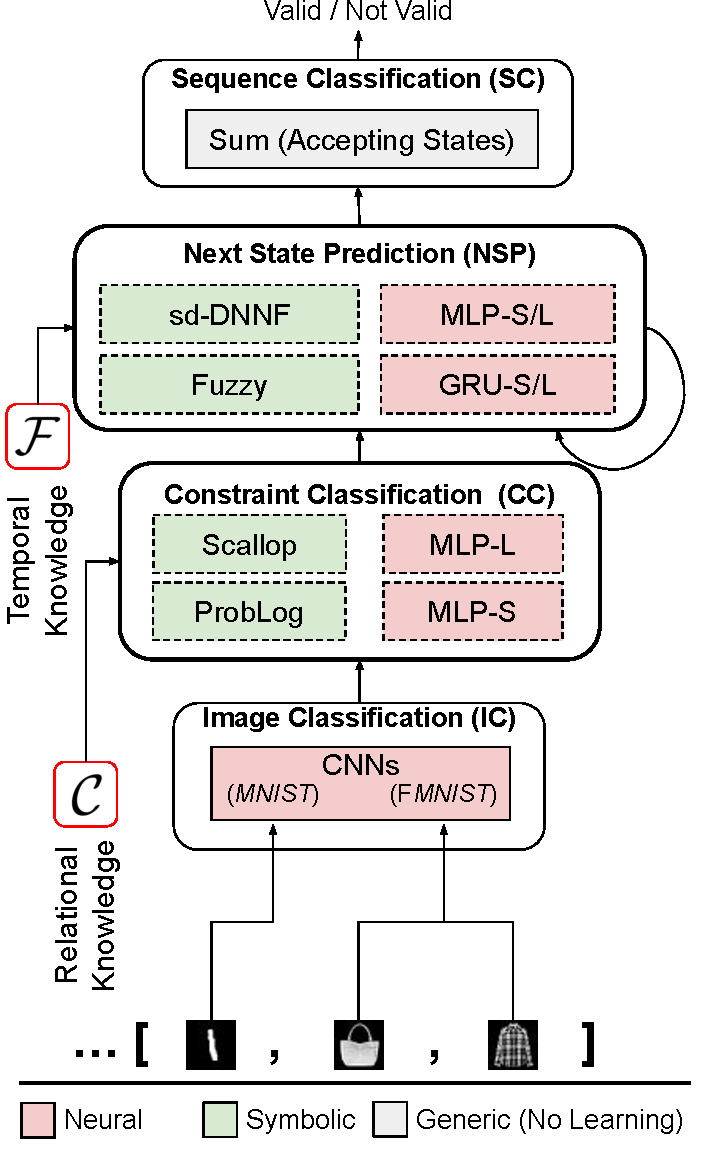
\includegraphics[width=0.4\linewidth]{imgs/ltlzinc/Zinc_fig.pdf}
	\caption[Modular architecture for LTLZinc]{Stages of our architecture for sequence classification experiments. We implemented {\sc cc} and {\sc nsp} in multiple ways (green: symbolic, reddish: neural).}
	\label{ltlzinc:fig:pipeline}
\end{figure}

We model the whole sequence classification task by a multi-stage pipeline composed of the following sub-tasks (Figure~\ref{ltlzinc:fig:pipeline}), which mimic the knowledge structure of \textsc{LTLZinc}: ({\sc\small ic}) \textit{image classification}, mapping data from each perceptual domain to the corresponding symbolic domain; ({\sc\small cc}) \textit{constraint classification}, leveraging ``relational'' knowledge; ({\sc\small nsp}) \textit{next state prediction}, leveraging ``temporal'' knowledge; ({\sc\small sc}) \textit{sequence classification}, i.e., the binary classification head. The full architecture is described in Appendix~\ref{app:ltlzincarc}. Appendix~\ref{app:ltlzinchyper} contains the choice of hyper-parameters for these experiments.

\paragraph{{\sc (ic)} Image Classification.} The first stage corresponds to a traditional Neural-network-based Image Classification task, estimating the probability of the symbol/class assignment $\phi_\vtheta: \gX^{(t)} \mapsto \gY^{(t)}$, corresponding to class probabilities $P^{(t)}_{\text{\sc\tiny ic}}(\langle y_{0}^{(t)}, \ldots, y_{|\gY|-1}^{(t)}\rangle \mid \langle x_{0}^{(t)}, \ldots, x_{|\gY|-1}^{(t)}\rangle)$. 
Since the proposed \textsc{LTLZinc-Sequential} tasks consist of perceptually simple images, our implementation is based on a small convolutional architecture, sharing parameters for each perceptual domain.\footnote{e.g., for Task 4 of \textsc{LTLZinc-Sequential-Short}, we have two instances of the same architecture: one to predict symbol $X$ from the MNIST domain and another one for symbols $Y, Z$ belonging to the Fashion MNIST domain, while for Task 5 a single instance is exploited for all the variables $W, X, Y, Z$, as they all belong to the MNIST domain.}

\paragraph{{\sc (cc)} Constraint Classification.} The set of all the image classes predicted by the \textsc{ic} module, is mapped to truth assignments for the relational constraints in $\gC$, each of them indicated with $c_i$. This stage estimates $P^{(t)}_{\text{\sc\tiny cc}}(\langle c_{0}^{(t)}, \ldots, c_{|\gC| - 1}^{(t)}\rangle \mid \langle y_{0}^{(t)}, \ldots, y_{|\gY|-1}^{(t)}\rangle)$. As relational knowledge is explicitly provided in our setting, this mapping can be implemented with any (i.) \textit{knowledge injection} technique, or (ii.) \textit{learned from observations}. 
Although \textsc{LTLZinc} as a framework can be more expressive, tasks in \textsc{LTLZinc-Sequential} are characterized by constraints which can be expressed in Datalog. To encode such constraints we selected Scallop~\cite{li2023scallop},\footnote{In initial explorations, the default top-$k$ proofs provenance ($k=1$) resulted in the best trade-off between inference time and accuracy.} and ProbLog~\cite{de2007problog}, to compare the effects of approximate and exact probabilistic inference.
Scallop and ProbLog programs are differentiable end-to-end, however they do not possess trainable parameters. To increase module flexibility, we augment our architecture with a set of additional learnable calibration parameters, which independently apply temperature rescaling to both input and output probabilities, each with their own independent weight. 
Learning temperature parameters takes place jointly with the \textsc{ic} module, and it allows us to control both the entropy of the distributions and the confidence of prediction, while preserving the argmax. In order to address possible numerical stability issues, we equip symbolic modules with probability (denoted with a -P suffix in subsequent tables) and log-probability (-LP suffix) semirings.
%
We compare symbolic methods with Multi-layer Perceptrons equipped with 64, or 8 hidden neurons (referred to as MLP-L and MLP-S, respectively).

\paragraph{{\sc (nsp)} Next State Prediction.} The temporal reasoning component is rooted on the definition of a discrete space of $M$ elements, each consisting of a state of the Symbolic Finite-state Automaton equivalent to the temporal specification $\gF$, based on the observed validity values of relational constraints, $c_i^{(t)}$. 
In this way, the temporal reasoning task is reduced to a next-state prediction problem, i.e., a recurrent classification problem where $s^{(t)} \in [0, M-1]$ is the predicted next-state, with probability $P^{(t)}_{\text{\sc\tiny nsp}}(s^{(t)} \mid \langle c_{0}^{(t)}, \ldots, c_{|\gC|-1}^{(t)}\rangle, s^{(t-1)})$.\footnote{Here and in the following, $t = -1$ is the initial instant, where the automaton of the \textsc{nsp} module is initialized to state ``$0$''.} 
We compare two neural and two symbolic approaches.
For the learning-based approaches we explore Multi-layer Perceptrons and Gated Recurrent Units, equipped with either 64 hidden/state neurons (MLP-L, GRU-L) or 8 hidden/state neurons, (MLP-S, GRU-S).
Gated Recurrent Units are augmented with a simple encoder-decoder, to convert the continuous hidden state into $M$ discrete classes.
For the symbolic approaches, we encode the ground truth as Deterministic Finite-state Automata, following the works of Umili et al.~\cite{umili2023grounding} and Manginas et al.~\cite{manginas2024nesya}. 
In their works, automata are encoded as a set of propositional logic formulae in the form $\texttt{prev\_state} \wedge \texttt{trans\_label} \rightarrow \texttt{next\_state}$, encoded by Logic Tensor Networks~\cite{badreddine2022logic} (here named Fuzzy) and sd-DNNFs~\cite{darwiche2002knowledge}, respectively. The output of symbolic reasoning is fed back as input, in a recurrent fashion.
As in the \textsc{cc} module, automata-based \textsc{nsp}'s predictions are temperature-calibrated by learnable parameters, jointly learned with the rest of the trainable parameters.

\paragraph{{\sc (sc)} Sequence Classification.} The final output $s^{(T-1)}$ of {\sc nsp} directly encodes the final state of the automaton. Hence, we can perform sequence classification in closed form: $P_{\text{\sc\tiny sc}}(f(\gS) = 1 \mid s^{(T-1)}) = \sum\limits_{a \in \text{\sc\tiny accepting}} P(s^{(T-1)} = a)$. 

\paragraph{Training the Pipeline.}
The four stages are combined into: 
\begin{equation}
	\nonumber
	P(f(\gS) = 1) = \left( \prod_{t=0}^{T-1} P^{(t)}_{\text{\sc\tiny ic}} P^{(t)}_{\text{\sc\tiny cc}} P^{(t)}_{\text{\sc\tiny nsp}} \right) P_{\text{sc}}(f(\gS) = 1 \mid s^{(T-1)}),
\end{equation}
where $P^{(t)}_{\bullet}$ is the shorthand notation for the already introduced probabilities with arguments at time $t$.
We train our multi-stage architectures with four loss functions, each weighted by a $\lambda_{\bullet}$ hyper-parameter. \textsc{ic} and \textsc{nsp} (the latter conditioned on the previous state) exploit a Categorical Cross-entropy loss, while \textsc{cc} and \textsc{sc} are subject to a Binary Cross-entropy loss.
Preliminary experiments demonstrated that training diverges due to extremely low initial confidence in image classification,\footnote{This is especially true when the \textsc{cc} module is a Scallop/ProbLog program, as at the beginning of training, misclassified images lead to confidently predicting violated constraints most of the time.} making the optimizer unable to converge, except in very simple tasks. This behavior is well known in the literature~\cite{manhaeve2021approximate,van2024independence,maene2024hardness}. 
To overcome this issue, we bootstrap the \textsc{ic} module with a pre-training phase, using the \textsc{ic}-loss only, to ensure a good starting image classification.

\section{Analysis of Neuro-Symbolic Stages}
The purpose of the modular architecture shown in Figure~\ref{ltlzinc:fig:pipeline} is to investigate the effect of interactions betweeen different reasoning methods. We will now briefly discuss the expected behavior of Neuro-symbolic combinations (i.e., neural \textsc{ic}, symbolic \textsc{cc} and symbolic \textsc{nsp}), in light of their semantics.
Our architecture is a feed-forward pipeline of stages with a unified input-output interface: each stage takes continuous inputs in the range $[0, 1]$ (with the exception of \textsc{ic}), and returns outputs in the same range.
Modules with different semantics can be mixed and matched (e.g., neural \textsc{ic}, Scallop \textsc{cc} and Fuzzy \textsc{nsp}) by means of this unified interface.
It is however important to note that the correctness of each module is based on specific assumptions, in particular, many probabilistic systems rely on input variables which are independent~\cite{van2024independence} to compute correct output probabilities. Specifically the \textsc{nsp} probabilistic module considered here (sd-DNNF) does make this assumption.
%
We shall now consider a numerical example from the task of Section~\ref{ltlzinc:sec:seqtasks} to demonstrate our NeSy infrastructure. Consider the following probability distributions computed by the neural component (\textsc{ic}) of the
system for the input $(\mathimg{mnist2}, \mathimg{svhn1}, \mathimg{cifarhor})$:
$$
\begin{aligned}
	P_{A}(A \mid \mathimg{mnist2}) &= \mathrm{Categorical}(
	[0.05, 
	0.00, 
	0.50, 
	0.00, 
	0.30, 
	0.00, 
	0.10, 
	0.05, 
	0.00, 
	0.00 
	])
	\\
	P_{B}(B \mid \mathimg{svhn1}) &= \mathrm{Categorical}(
	[0.00, 
	0.80, 
	0.00, 
	0.10, 
	0.10, 
	0.00, 
	0.00, 
	0.00, 
	0.00, 
	0.00 
	]) \\
	P_{C}(C \mid \mathimg{cifarhor}) &= \mathrm{Categorical}(
	\underbrace{
		[0.15,
		0.00, 
		0.00, 
		0.00, 
		0.05, 
		0.00, 
		0.00, 
		0.80, 
		0.00, 
		0.00]
	}_{\text{airplane, automobile, bird, cat, deer, dog, frog, horse, ship, truck}}
	).
\end{aligned}
$$
The domains of the variables $\langle A, B, C \rangle$ are given in Section \ref{ltlzinc:sec:seqtasks}: the first two variables simply take values from $[0, 9]$, while the domain of the third is an enumeration (indicated below the vector of probabilities), which can also be mapped to $[0, 9]$.
Consider now the constraint $\texttt{p}(A, B, C): A = 2 \cdot B \vee \ B = 2 \cdot C$ from the example in Section \ref{ltlzinc:sec:seqtasks}. 
Its probability can be computed via:
$$
\begin{aligned}
	P(\texttt{p}(A, B, C)) &= \sum_{A, B, C} 
	P_{a}(A = a \mid \mathimg{mnist2}) 
	P_{b}(B = b \mid \mathimg{svhn1}) 
	P_{c}(C = c \mid \mathimg{cifarhor}) 
	\llbracket \texttt{p}(A, B, C) = \top \rrbracket \\
	&= \boxed{
		P_A(A = 2 \mid \mathimg{mnist2}) 
		\cdot  P_B(B = 1 \mid \mathimg{svhn2}) 
		\cdot P_C(C = \mathrm{horse} \mid  \mathimg{cifarhor})} \\
	&+  P_A(A = 6 \mid \mathimg{mnist2}) \cdot  P_B(B = 3 \mid \mathimg{svhn2}) \cdot P_C(C = \mathrm{horse} \mid \mathimg{cifarhor})
	+ \dots \\
	&= \boxed{0.5 \cdot 0.8 \cdot 0.8} + 
	0.1 \cdot 0.1 \cdot 0.8 + \dots \\
	&= \boxed{0.32} + 0.09 + \dots \\
	&= 0.41
\end{aligned}
$$
where $\llbracket \cdot \rrbracket$ is an indicator function, which filters assignments based on whether they satisfy the constraint. The computation above bears strong 
resemblance to that of Weighted Model Counting. %, which is exploited by various 
%neuro-symbolic systems.
Since these possible worlds for complex constraints can be exponential in the number 
of input variables, involved techniques have been developed to answer such queries effectively, either in an exact fashion~\cite{darwiche2002knowledge, de2007problog} (our ProbLog \textsc{CC} module) or by only considering high probability proofs~\cite{manhaeve2021approximate,li2023scallop} (our Scallop \textsc{cc} module). 
The boxed term above is the most probable world for the query $\texttt{p}(A, B, C)$ with a probability mass of $0.32$. 
Similar computations hold for $\texttt{q}(A, B) : \texttt{all\_different}([A, B])$ and $\texttt{r}(C): C \in \left\{\text{bird}, \text{cat}, \text{deer}, \text{dog}, \text{frog}, \text{horse}\right\}$. To summarize, the following are the probabilities for our example, as the sum of the most possible world (boxed) and the residual 
given by lower probability worlds:
\begin{align*}
	P(\texttt{p}(A,B,C)) &= \boxed{0.32} + 0.09 = 0.41\\
	P(\texttt{q}(A,B)) \quad &= \boxed{0.4} + 0.57 = 0.97\\
	P(\texttt{r}(C)) \quad\quad &= \boxed{0.8} + 0.05 = 0.85.
\end{align*}
It can be noted how the approximation error of considering only the most probable possible
world (Scallop \textsc{cc} module) instead of all the possible worlds (ProbLog \textsc{cc} module) can be significant.
%
We now turn to the issue of independence. For our example, $\texttt{p}(A,B,C)$ and $\texttt{q}(A, B)$ share variables and possible worlds, therefore they are not independent. Similarly, for $\texttt{p}(A, B, C)$ and $\texttt{r}(C)$. However 
$\texttt{q}(A, B)$ and $\texttt{r}(C)$ are independent because they share no variables.
Let us now consider the interaction between the probabilities of the \textsc{cc} module and the probabilities computed via the \textsc{nsp} module, on two transition examples from the automaton of Figure~\ref{ltlzinc:fig:example-dfa}. The transition $[2\rightarrow4]: \neg \texttt{q}(A, B) \wedge \texttt{r}(C)$ corresponds to the conjunction of independent events, while constraints appearing in transition $[1\rightarrow2]: \neg \texttt{p}(A,B,C) \wedge \neg \texttt{q}(A, B)$ are dependent. Note that, from the perspective of the \textsc{nsp} module, the proof tree is lost and that \texttt{p}, \texttt{q} and \texttt{r} are now input variables.
Let the \textsc{nsp} module be implemented via an exact probabilistic implementation (sd-DNNF): both transitions are computed as products of probabilities.
We have $P([2\rightarrow4]) = (1 - P(\texttt{q}(A, B))) \cdot P(\texttt{r}(C))$, corresponding to $0.48$ if the \textsc{cc} module yielded only the top proof probability, and $0.0255$ in the case of exact probabilities. As these constraints are independent, these results correspond to those obtained by Weighted Model Counting if we had the proof tree available (i.e., if the \textsc{cc} and \textsc{nsp} module were a single module with access to input variables $A, B, C$).
For the second transition, the \textsc{nsp} module computes probabilities in the same fashion: $P([1 \rightarrow 2]) = (1 - P(\texttt{p}(A, B, C)) \cdot (1 - P(\texttt{q}(A, B)))$, returning $0.408$ (top proof) or $0.0177$ (exact). However, a monolithic probabilistic implementation would not ignore the
dependence between $\texttt{p(A, B, C)}$ and $\texttt{q(A, B)}$ and would, in exact mode, compute the probability as $0.03 \neq 0.0177$.
%
The approximation error, caused by the violation of the independence assumption at the \textsc{nsp} level, compounds with the one caused by selecting only the top proof within the \textsc{cc} module. In this thesis we mitigate this error in a data-driven fashion by means of temperature calibration and intermediate level supervisions.
A natural alternative would be to implement a monolithic \textsc{cc-nsp} module, capable of computing transition probabilities from image labels in an end-to-end fashion. This approach however introduces additional scalability and optimization challenges which we reserve to address in future work.


	

	
\iffalse	
	\section{Methodology}
	\label{ijcai:sec:setup}
	
	%\subsection{Setup}\label{ijcai:sec:setup}
	We model the whole sequence classification task by %cascading multiple decisions.
	%
	% In particular, we employ 
	a multi-stage pipeline composed of the following sub-tasks, also sketched in Fig.~\ref{ltlzinc:fig:pipeline}: ({\sc\small ic}) image classification, mapping data from each $\mathcal{X}_i$ to the corresponding $\mathcal{Y}_i$; ({\sc\small cc}) constraint classification, leveraging ``relational'' knowledge; ({\sc\small nsp}) next state prediction, leveraging ``temporal'' knowledge; ({\sc\small sc}) sequence classification, i.e., the binary classification problem.
	%
	LTLZinc provides annotations for each of these sub-tasks, so that we can evaluate performance both in isolation for each component, and jointly in an end-to-end fashion%. At the same time, such annotation richness allows to
	, while also being able to define multiple training objectives, applied at different stages.
	%
	%Note that the first three stages \smc{({\sc\small ic}, {\sc\small cc}, {\sc\small nsp})} can be implemented by time-agnostic predictors in a straightforward way, by simply learning a classic input-output mapping. Even the last stage \smc{({\sc\small sc})} can be performed in a time-agnostic fashion, by capitalizing on the equivalence between LTL over finite traces and DFAs~\cite{de2013linear}, and performing sequence classification algorithmically, just by iterating next state prediction and checking whether the last element of the trace is an accepting state for the underlying automaton.
	%%%
	We %leverage LTLZinc to 
	address the following research questions.
	
	\noindent\fbox{%
		\parbox{0.96\columnwidth}{%
			\small
			\textbf{Q1: Can neural-only methods solve the proposed tasks?} Given enough training capacity, can a neural network successfully perform sequence classification, without background knowledge?\\
			\textbf{Q2: How do neural-only and neuro-symbolic methods compare?} Can background knowledge mitigate error amplification issues along multiple stages? Are neuro-symbolic methods more prone to training instability than neural-only approaches? \\
			\textbf{Q3: What is the effect of upstream noise on exact symbolic methods?} Do wrong, but confident, predictions of symbols $y_i$'s affect downstream accuracy more than correct predictions associated with lower confidence? How is noise propagated? %through the symbolic modules?
		}%
	}
	
	\iffalse
	\textbf{Q1: Can neural-only methods solve the proposed tasks?} Given enough training capacity and trainable parameters, can a neural network successfully perform sequence classification, without exploiting background knowledge? %\OLD{Does conditioning each stage with the (possibly incorrect) output of the previous one have any effect on learning?}
	
	\textbf{Q2: How do neural-only and neuro-symbolic methods compare?} Can background knowledge overcome the issues caused by error amplification along our multi-stage architecture? Are neuro-symbolic methods more prone to training instability than neural-only approaches? 
	
	\textbf{Q3: What is the effect of upstream noise on exact symbolic methods?} Do wrong, but confident, predictions of symbols $y_i$'s affect downstream accuracy more than correct predictions associated with lower confidence? %\smc{NOTA Stefano: non capisco bene la domanda precedente, forse perche' non mi e' chiaro chi fa le predictions e dove si misura la downstream accuracy?}
	%\lsl{La domanda in realtà serve a giustificare la risposta che diamo in sec. 6 con le ablations. Ci sono due tipi di oracoli (che vanno a sostituire pezzi di  architettura da un certo punto in poi), uno che ogni tanto sbaglia label, ma ha sempre confidence 1.0, l'altro  che dà sempre la label giusta (come argmax), ma ha confidence più bassa.  In termini di XAI ci piacerebbe che il secondo andasse meglio, ma gli esperimenti mostrano che il primo funziona meglio (inteso come accuracy finale più alta) nel nostro  setting.  Le accuracy che misuriamo sono sui vincoli e sul next state dell'automa}
	How is noise propagated through the symbolic modules?
	\fi
	
	%\paragraph{Stages.} 
	%\subsection{Models}
	%\lsl{Luca: Like for Section 4, I would try to remove  subsections.}
	%We address knowledge-driven classification by composing four stages, where the output of each is fed to the next.
	%\noindent We create the context to address these questions by detailing the stages of the computational pipeline we implemented.
	%We address knowledge-driven classification in four stages, connecting the output of each to the input of the next.
	
	\paragraph{{\sc (ic)} Image classification.} The first stage corresponds to a traditional neural-based image classification task, estimating the probability of the class assignment $[y_{0}^{t}, \ldots, y_{N-1}^{t}]$, i.e., $P_{\text{\sc\tiny ic}}([y_{0}^{t}, \ldots, y_{N-1}^{t}] \mid [x_{0}^{t}, \ldots, x_{N-1}^{t}])$. %, and it can thus be implemented by a fully neural component. 
	%Since the proposed LTLZinc tasks (Appendix \ref{ijcai:app:tasks}) consist of perceptually simple images, o
	Our implementation is based on a convolutional architecture (details in Appendix~\ref{ijcai:app:backbone}), for each perceptual domain % across variables grounded in the same domains 
	(e.g., for the example of Section~\ref{ijcai:sec:seq}, we have two instances of the same architecture: one to predict symbols $y_A, y_B$ (MNIST categories) and another one for symbols $y_C$ (SVHN categories), see Fig.~\ref{ltlzinc:fig:pipeline}).
	
	\paragraph{{\sc (cc)} Constraint classification.} The set of all the image classes  %$\{y_j \in \mathcal{Y}_j \mid j \in [0, |\mathcal{Y}_j| - 1]\.}$, r
predicted by the \textsc{ic} module, is mapped to $|\mathcal{C}|$ validity values, %$\{\beta_i \in [0, 1] \mid i \in [0, |\mathcal{C}| - 1]\}$, 
each of them indicated with $\beta_i$, one for each of the constraints defined in the relational knowledge $\mathcal{C}$. This stage estimates $P_{\text{\sc\tiny cc}}([\beta_{0}^{t}, \ldots, \beta_{|\mathcal{C}| - 1}^{t}] \mid [y_{0}^{t}, \ldots, y_{N-1}^{t}])$. %As 
%constraints 
%relational knowledge is
%are 
%explicitly provided in our setting, this map %equation 
%can be implemented with any knowledge injection technique.
%Although LTLZinc is strictly more expressive than Scallop, 
Our experiments focus on tasks characterized by constraints which can be expressed in Datalog.
Hence, we chose Scallop~\cite{li2023scallop}, a neuro-symbolic engine capable of probabilistic reasoning over Datalog programs, supporting inference over multiple provenance semirings~\cite{green2007provenance}.\footnote{In initial explorations, the default top-$k$ proofs provenance ($k=1$) resulted in the best trade-off between inference time and accuracy.} %Although LTLZinc is strictly more expressive than Scallop, our experiments focus on tasks characterized by constraints which can be expressed in Datalog. %\footnote{In principle, other more expressive frameworks, such as DeepProbLog, could be used as well.}
Scallop programs are differentiable end-to-end, however they do not possess trainable parameters. To increase module flexibility, we augment our architecture with an optional set of additional learnable calibration parameters %calibration weights 
(enabled by a ``calibrate'' hyper-parameter in the experiments of Section \ref{ijcai:sec:exp}), which independently apply temperature rescaling to both input and output probabilities. %, each with their own independent weight. 
Learning takes place jointly with the \textsc{ic} module, and it allows us to control both the entropy of the distributions and the confidence of prediction, while preserving the argmax.
\iffalse
$\tau > 0$,
\begin{equation}
	\begin{cases}
		P'_{in}(logits) = \mathrm{softmax}\left(\frac{\mathrm{logits}}{\tau + \epsilon}\right) & \text{for input labels}\\
		P'_{out}(P) = \sigma\left(\frac{\sigma^{-1}(P)}{\tau + \epsilon}\right) & \text{for output probabilities},
	\end{cases}
\end{equation}
where $\mathrm{logits}$ is the output of the last linear projection of the \textsc{ic} module, and $\epsilon$ is small positive constant. Intuitively, these equations apply an activation function after rescaling their argument. Since the top-$k$ provenance in Scallop returns probabilities, $P'_{out}$ requires an inverse mapping in logit space before scaling.
\smc{{\bf * Stefano's note *} define logts and explian these equations)} \lsl{Luca: better now?}
\ml{MARCO: are we sure this is necessary? Maybe move to appendix? Looks like a technicality...}
\fi
%Temperature scaling preserves the argmax. % while reshaping the output distribution, controlling both the entropy of the distribution and the confidence of prediction. 
%\smc{{\bf * Stefano's note *} it would require more details here, maybe we can simplify the previous sentence?}
%In contrast with traditional confidence calibration approaches, %where temperature is calibrated on a separate validation set %, after fixing the main trainable parameters, as 
%(the Scallop classification module is already ``trained'', lacking any trainable weight), 
%we treat temperature parameters %as first class citizens and 
%as learnable parameters and train them jointly with the perceptual module. %, by using the training set.
%
We compare Scallop with two fully-learning-based approaches: a small multi-layer perceptron with limited capacity (8 hidden neurons, MLP-S) and a larger one (64 hidden neurons, MLP-L), see Appendix \ref{ijcai:app:constraints}.

\paragraph{{\sc (nsp)} Next state prediction.} The temporal reasoning component is rooted on the definition of a discrete space of $M$ elements, each consisting of a state of the DFA equivalent to $\mathcal{F}$, based on the observed validity values of relational constraints, $\beta_i^t$'s.
%is a recurrent \smc{function} updating an internal state $\alpha$ \smc{belonging to a discrete space of $M$ elements, each consisting of a state} of the DFA equivalent to the temporal specification $\mathcal{F}$. 
In this way, temporal reasoning is reduced to to a next-state prediction problem, i.e., a recurrent classification problem where $\alpha^t \in [0, M-1]$ is the predicted class/next-state, with probability $P_{\text{\sc\tiny nsp}}(\alpha^{t} \mid [\beta_{0}^{t}, \ldots, \beta_{\mathcal{V}-1}^{t}], \alpha^{t-1})$.\footnote{Here and in the following, $t = -1$ is the initial instant, where the automaton of the \textsc{nsp} module is initialized to state ``$0$''.} % (recurrent) classification task, 
%implemented with a recurrent network with discrete internal state $\alpha \in [0, M-1]$, i.e., one of the DFA possible states.} %as  a  each value is guaranteed to have a clear interpretation and we can frame next state prediction as a (recurrent) classification task.
%$ \in [0, M - 1]$, with $M$ being the number of states in the automaton corresponding to formula $\mathcal{F}$, 
%based on the observed \smc{validity values of relational constraints}, $\{\beta_i\}$. 
%We model the internal state as a discrete space, consisting of the states of the DFA equivalent to the temporal specification $\mathcal{F}$. In this way, each value is guaranteed to have a clear interpretation and we can frame next state prediction as a (recurrent) classification task.
%For the \textsc{nsp} module, 
We compare four learning-based approaches (two MLP's, namely MLP-S and MLP-L, and two gated recurrent units, GRU-S, GRU-L, with 8 and 64 hidden/state neurons, respectively), and four symbolic approaches.
GRUs are augmented with a simple encoder-decoder, to convert the continuous hidden state into $M$ discrete classes.
For the symbolic approaches, we encode the ground truth DFA, following~\cite{umili2023grounding} and~\cite{manginas2024nesya}. %In both cases, 
Such automaton is a set of propositional formulae as $\textsc{\small prev\_state} \wedge \textsc{\small trans\_label} \rightarrow \textsc{\small next\_state}$, encoded by logic tensor networks~\cite{badreddine2022logic} (here named Fuzzy) and sd-DNNF~\cite{darwiche2002knowledge}, respectively. To assess the effect of numerical stability, we performed computations both in probability space and log-probability space (suffixes -P and -LP, respectively).
%we instantiate both approaches in two flavors: one  performing computations in probability space (conjunctions implemented as multiplications, disjunctions as sums) and the other in log-probability space (conjunctions as sums, disjunctions as logsumexp operations). 
%See Appendix~\ref{ijcai:app:nextstate}.
As in the \textsc{cc} module, automata-based \textsc{nsp}'s predictions are optionally temperature-calibrated.

%We also briefly experimented with a Scallop implementation, however, it revealed to be intractably slow, not being able to perform inference over a single batch of constraints within a 2 hours time-out, with the exception of very small automata, far below the number of states and transitions required for the LTLZinc tasks explored in this work. This was the case also for approximate $\mathcal{O}(1)$ semirings, such as the max-mult provenance implemented in the standard Scallop library.

\paragraph{{\sc (sc)} Sequence classification.} The final output $\alpha^{T-1}$ of {\sc nsp} directly encodes the final state of the automaton. Hence, we can perform sequence classification in closed form: $P_{\text{\sc\tiny sc}}(f(\mathcal{S}) = 1 \mid \alpha^{T-1}) = \sum\limits_{s \in \text{\sc\tiny accepting}} P(\alpha^{T-1} = s)$. % = \sum_{s \in \text{\sc\tiny accepting}} P(\alpha^{T-1} = s)$.}.

\begin{figure*}
\centering
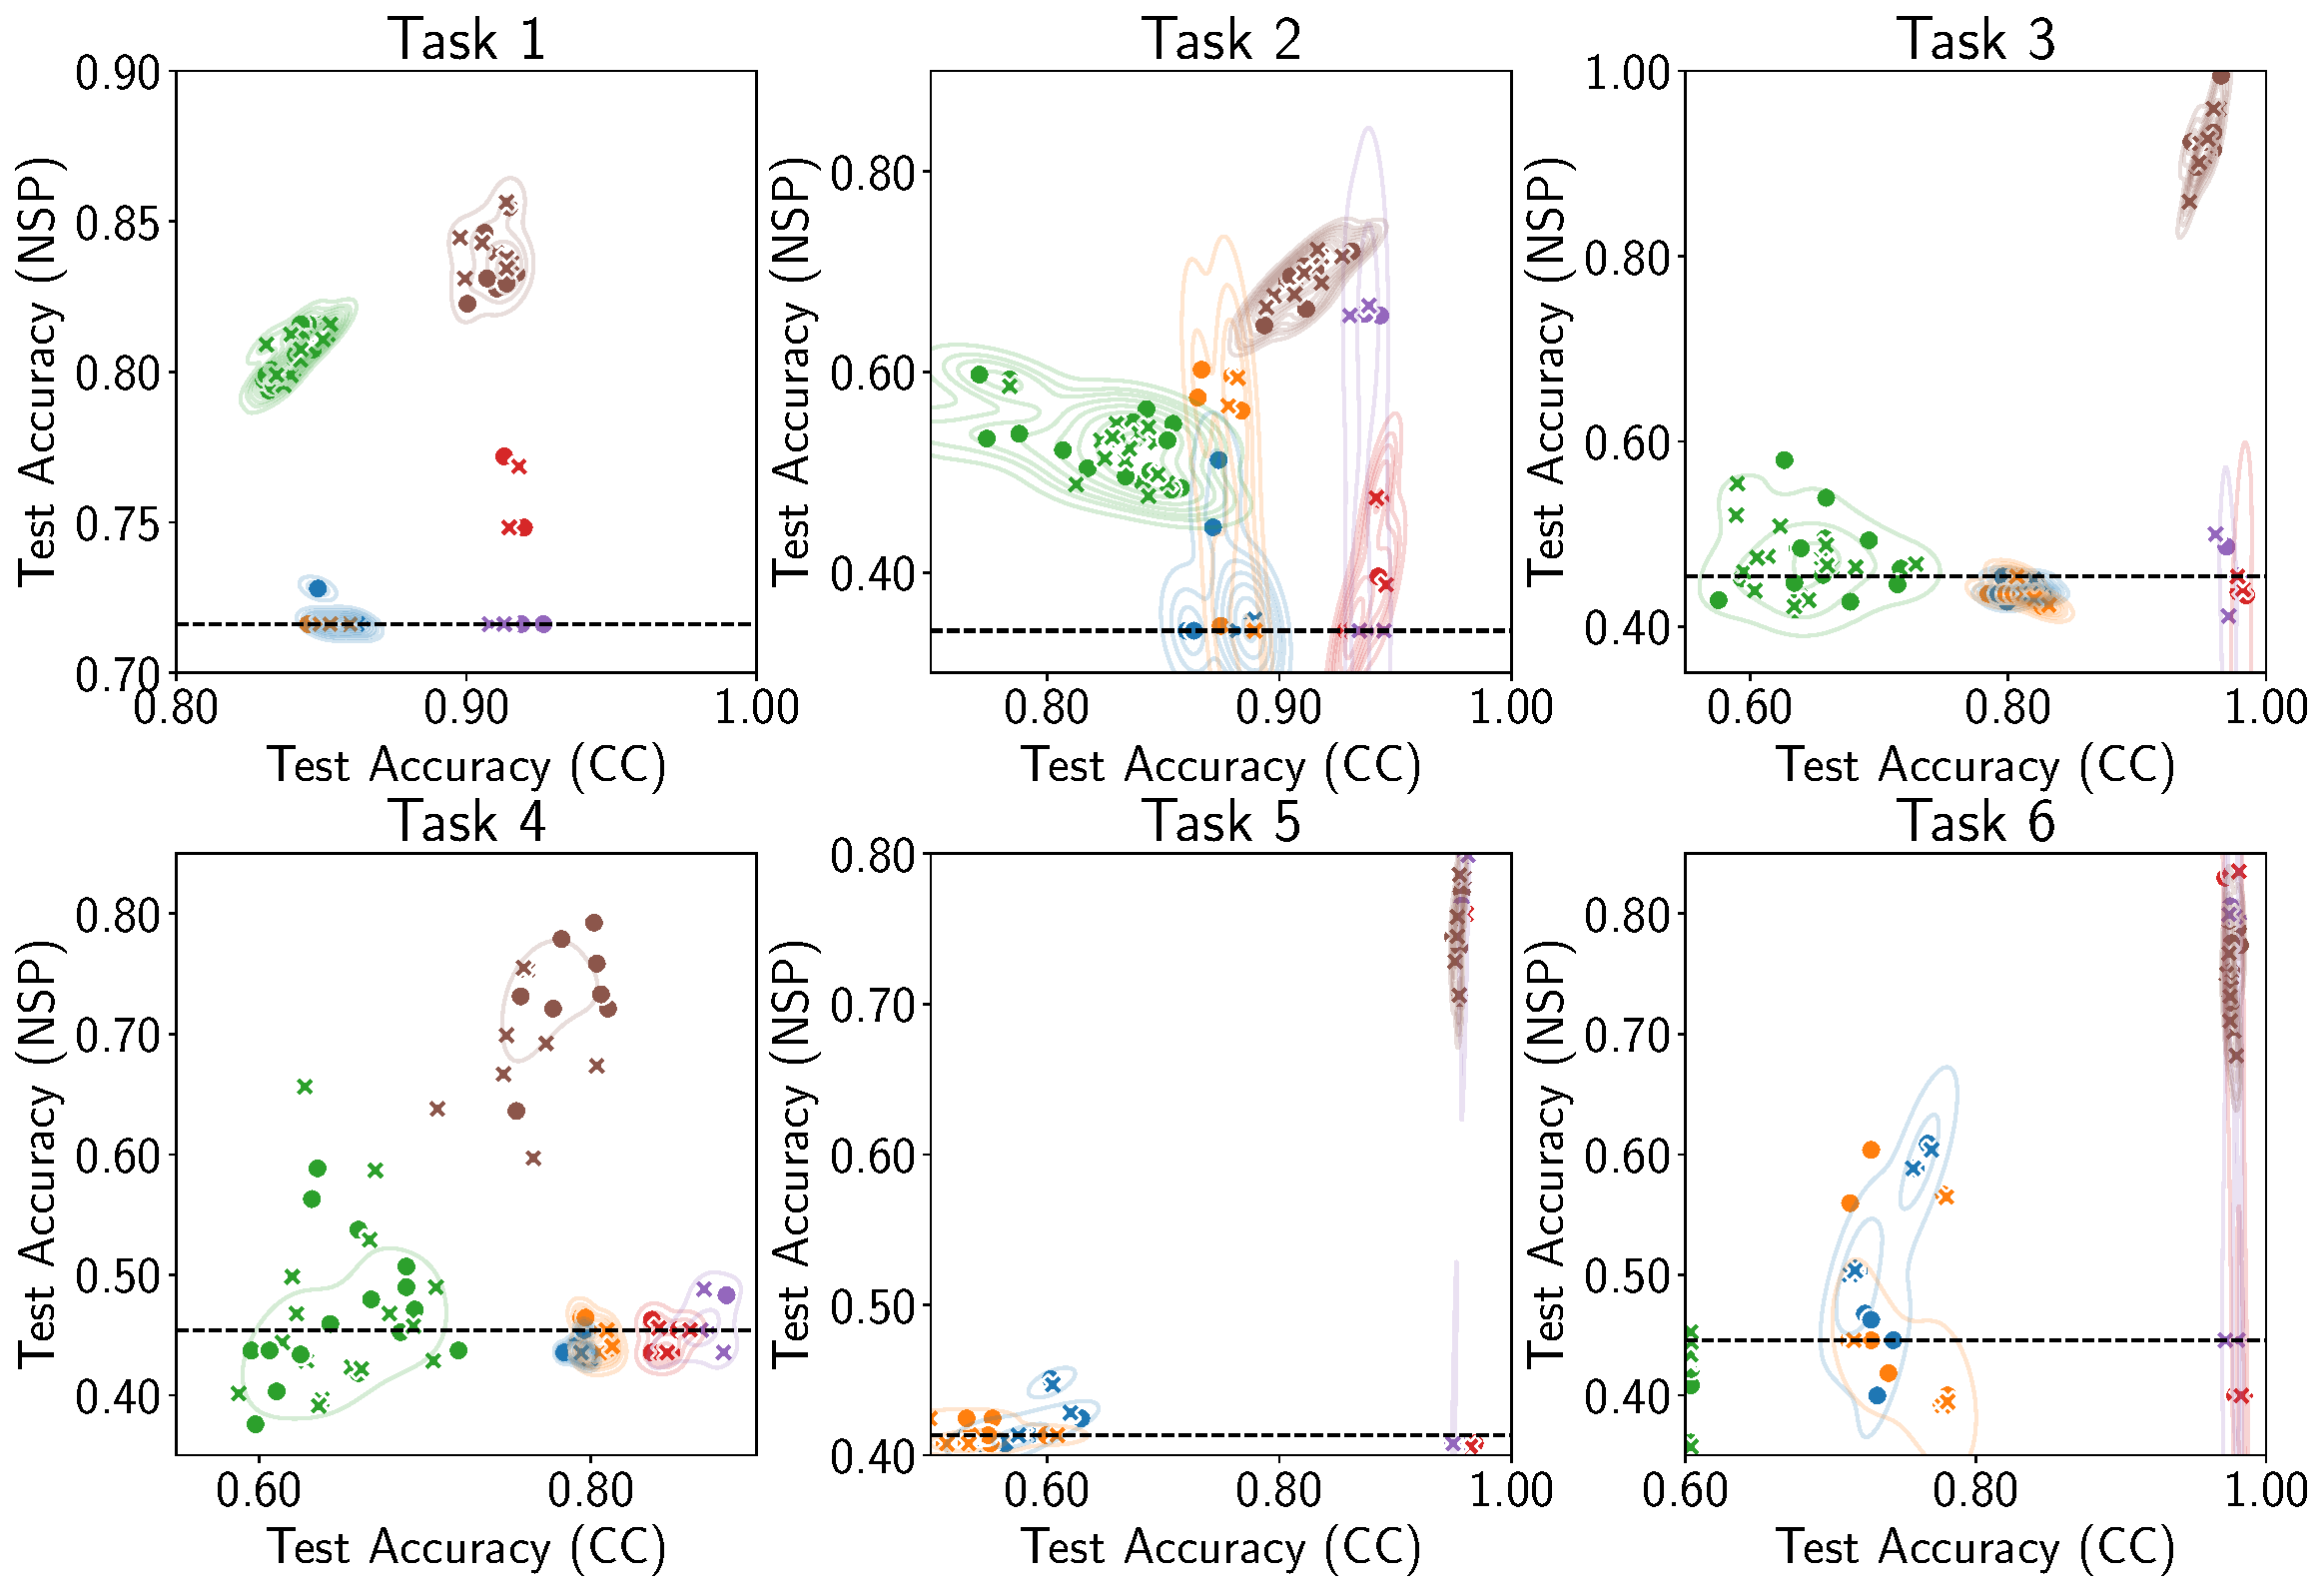
\includegraphics[width=1.0\textwidth]{imgs/ijcai/const-vs-succ.pdf}
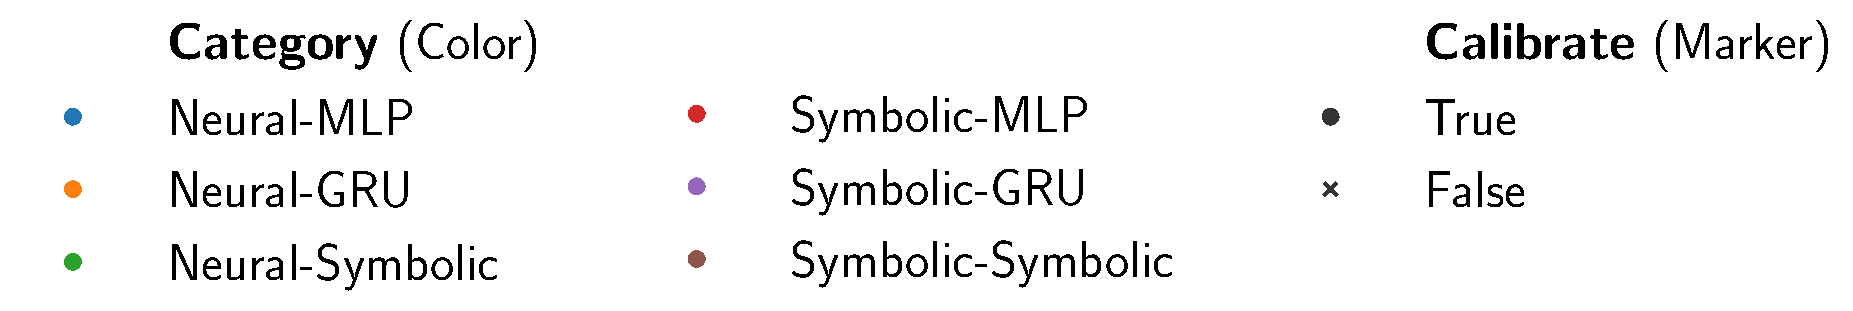
\includegraphics[width=1.0\textwidth]{imgs/ijcai/const-vs-succ_legend.pdf}
\caption[\textsc{cc}--\textsc{nsp} trade-off on LTLZinc-Short (rejection sampling)]{\textbf{Q2}. {\sc cc}-{\sc nsp} accuracy trade-off for different families of architectures (i.e., Neural/Symbolic {\sc cc}, MLP/GRU/Symbolic {\sc nsp}). The dashed line indicates the baseline performance of a deterministic {\sc nsp} always selecting the state most represented in the training set.} %Axes stretched for readability.}
\label{ijcai:fig:main}
\end{figure*}
%\paragraph{Building and training the pipeline.}
\paragraph{Training the pipeline.}
The four stages are combined into: %a single recurrent (with respect to $\alpha^t$) objective, %(where $sc$, $nsp$, $cc$, $ic$ stand for sequence classification, next state prediction, constraint classification and image classification, respectively):
%\begin{equation}
%\nonumber
$    P(f(\mathcal{S}) = 1) =  \left( \prod\limits_{t=0}^{T-1} P^t_{\text{\sc\tiny ic}} P^t_{\text{\sc\tiny cc}} P^t_{\text{\sc\tiny nsp}} \right) P_{\text{sc}}(f(\mathcal{S}) = 1 \mid \alpha^{T-1})$,
%\end{equation}
where $P^t_{\cdot}$ is the shorthand notation for the already introduced probabilities with arguments at time $t$.

%%%
%\paragraph{Losses.}
We train our multi-stage architectures with four loss functions, each weighted by a $\lambda_{\cdot}$ hyper-parameter. \textsc{ic} and \textsc{nsp} (the latter conditioned on the previous state) exploit a %modules are both subjected to a 
categorical cross-entropy loss, %and weighted by $\lambda_{ic}$ and $\lambda_{ns}$, respectively. 
while \textsc{cc} and \textsc{sc} %are evaluated against 
a binary cross-entropy loss. %, and weighted by $\lambda_{cp}$ and $\lambda_{sc}$, respectively. 
For \textsc{sc}, we also evaluate the semantic loss proposed by~\cite{umili2023grounding}.
%%%
%Traditionally, the neuro-symbolic task of distant supervision should be performed employing a small number of supervisions; %(roughly corresponding to $\lambda_{ic} \approx 0$ in our setting); 
%however, 
Preliminary experiments demonstrated that training diverges due to extremely low initial confidence in image classification,%\footnote{This is especially true when the \textsc{cc} module is a Scallop program, as at the beginning of training, misclassified images lead to confidently predicting violated constraints most of the time.} %, which do not provide useful gradients, unless coupled with image-level supervisions.} 
making the optimizer unable to converge, except in very simple tasks. This behavior is well known in the literature~\cite{manhaeve2021approximate,van2024independence,maene2024hardness}, and, in this paper, it only affects experiments aimed at investigating \textbf{Q2}, where we bootstrap the  \textsc{ic} module with a $5$ epochs pre-training phase, using the \textsc{ic}-loss only, %where we set $\lambda_{ic} = 1$, $\lambda_{cp} = \lambda_{ns} = \lambda_{sc} = 0$, 
to ensure a good starting image classification. %Note that for auxiliary experiments, no pre-training is required.
\fi


\section{Neural-only Experiments}
\begin{figure*}[htb!]
	\centering
	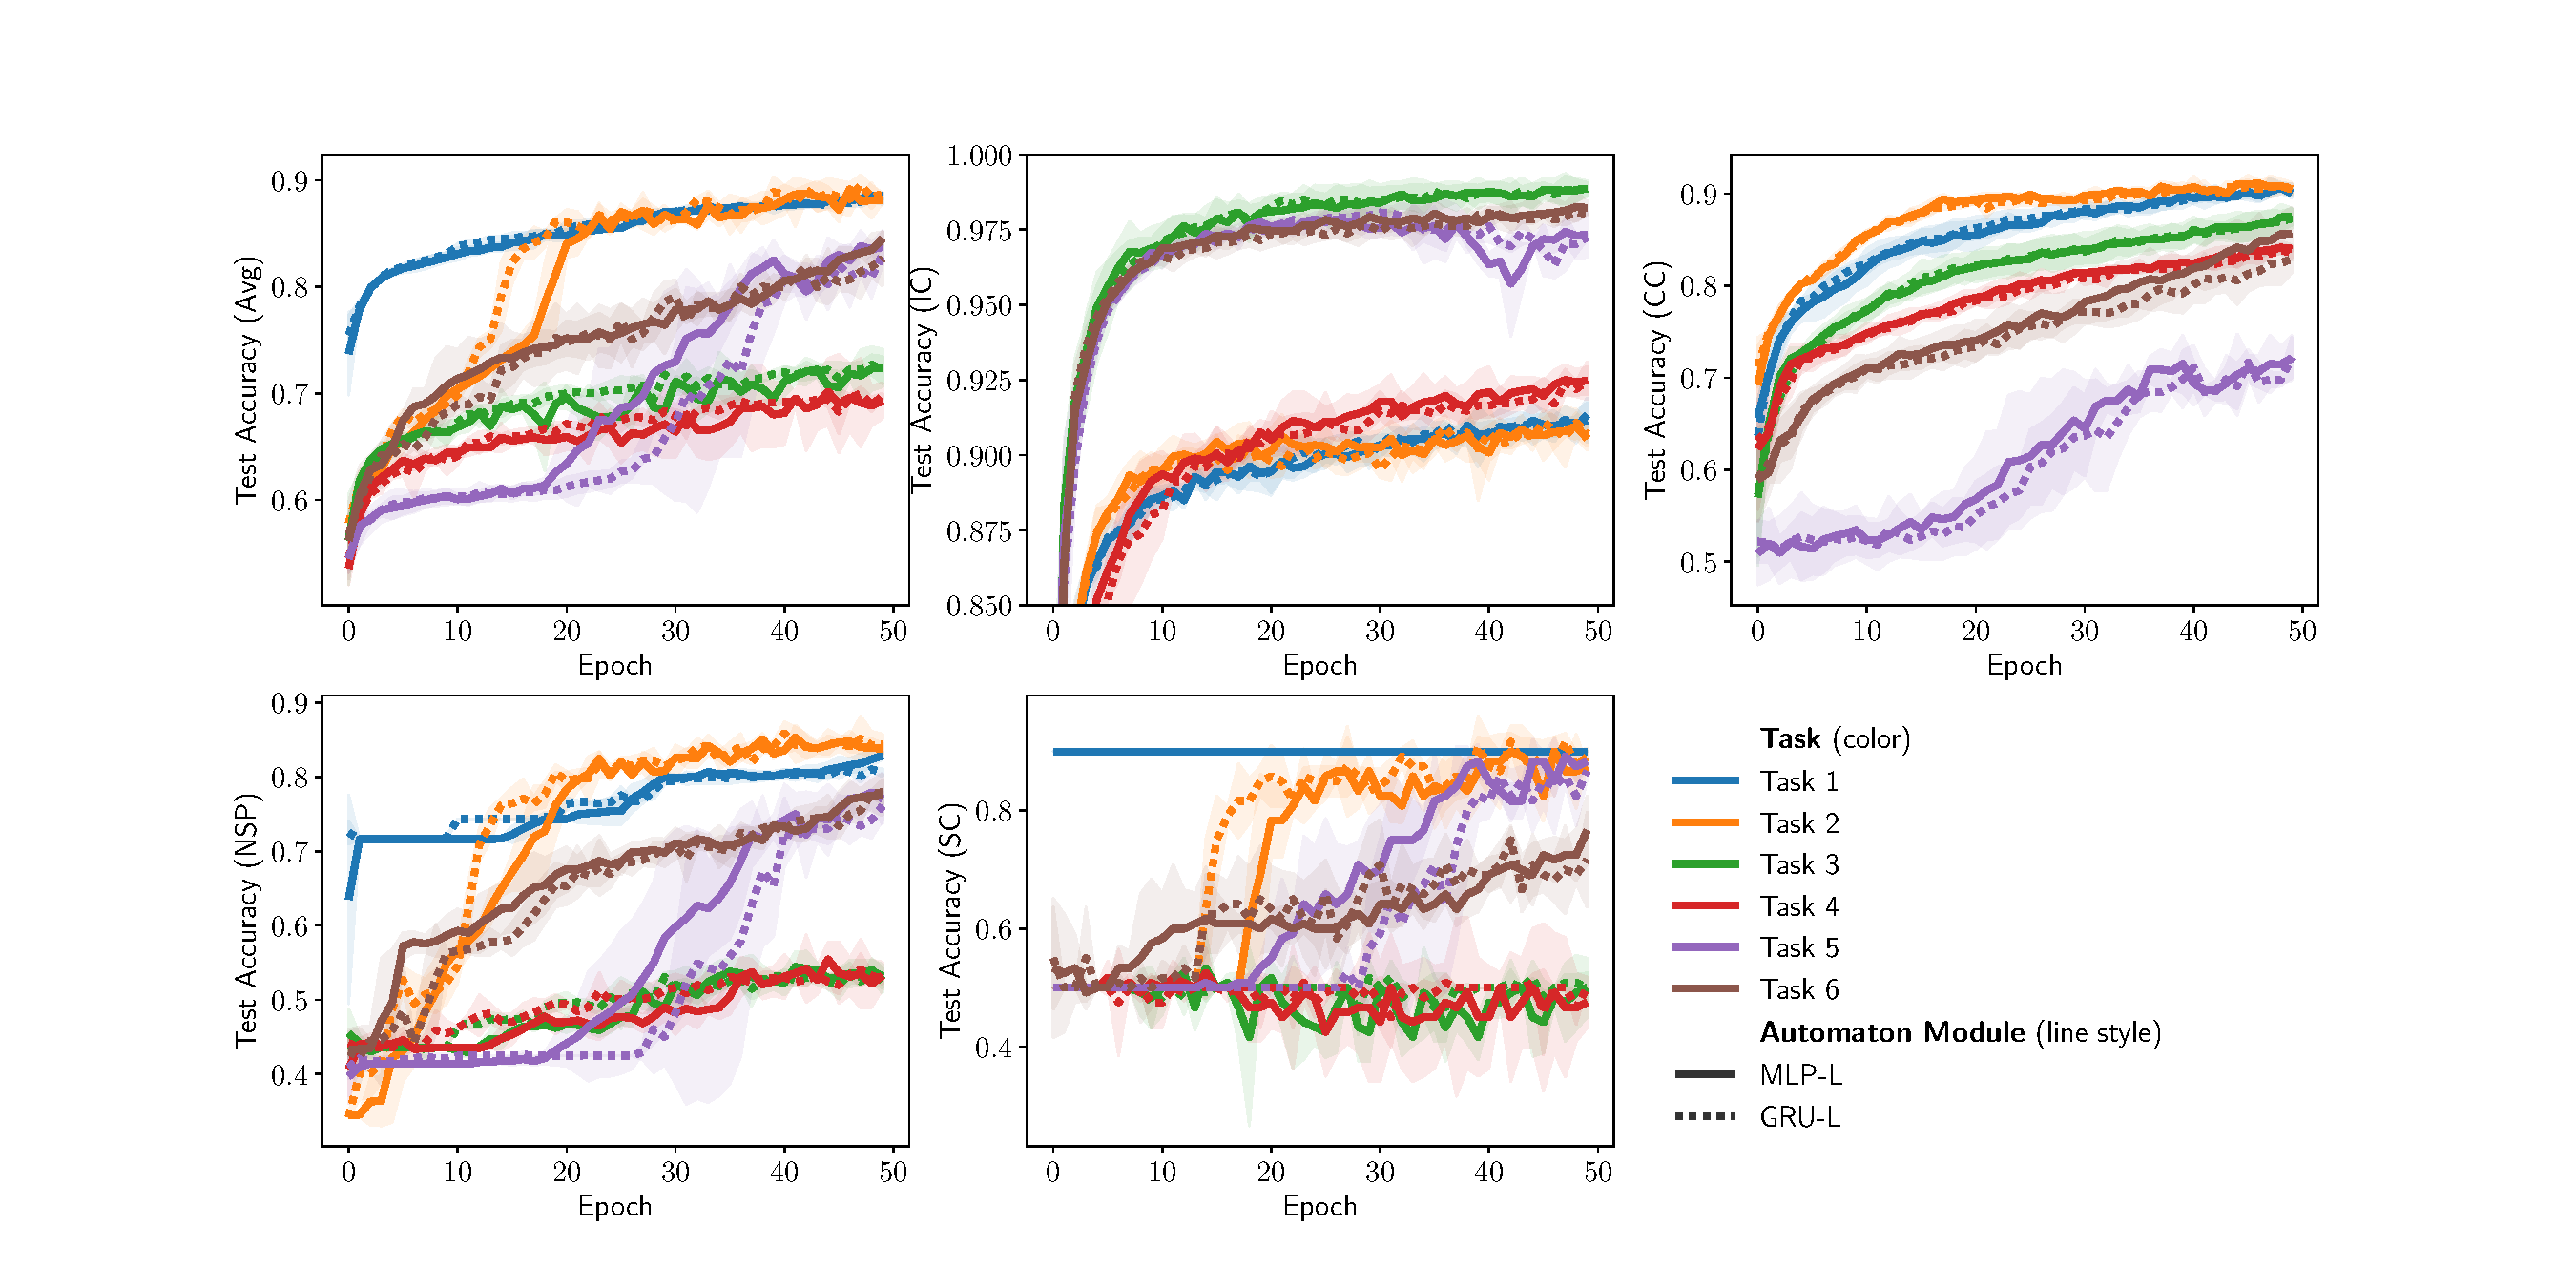
\includegraphics[width=\linewidth]{imgs/ijcai/task_validation.pdf}
	\caption[Neural-only experiments on \textsc{LTLZinc-Sequential-Short-Legacy}]{Test set dynamics for Neural-only experiments on \textsc{LTLZinc-Sequential-Short-Legacy}.}
	\label{fig:neural-only}
\end{figure*}

\begin{table*}[htb!]
	\centering
	\resizebox{\textwidth}{!}{
		\begin{tabular}{ccccccccc}
			\toprule
			\multirow{2}{*}{\sc Task} & \multirow{2}{*}{\shortstack[c]{\sc Automaton\\\sc Module}} & \multirow{2}{*}{\shortstack[c]{\sc Average\\\sc Accuracy}\raisebox{1ex}{\:$\uparrow$}} & \multirow{2}{*}{\shortstack[c]{\sc Label\\\sc Accuracy}\raisebox{1ex}{\:$\uparrow$}} & \multirow{2}{*}{\shortstack[c]{\sc Constraint\\\sc Accuracy}\raisebox{1ex}{\:$\uparrow$}} & \multirow{2}{*}{\shortstack[c]{\sc Successor\\\sc Accuracy}\raisebox{1ex}{\:$\uparrow$}} & \multirow{2}{*}{\shortstack[c]{\sc Sequence\\\sc Accuracy}\raisebox{1ex}{\:$\uparrow$}}
			& \multirow{2}{*}{\shortstack[c]{\sc Most Probable\\\sc Successor Acc.}\raisebox{1ex}{\:$\uparrow$}}
			& \multirow{2}{*}{\shortstack[c]{\sc Most Probable\\\sc Sequence Acc.}\raisebox{1ex}{\:$\uparrow$}}\\
			& & & & & & & & \\
			\midrule
			\multirow{2}{*}{\shortstack[c]{Task 1}} & MLP-L & $\textbf{0.89}$ & $0.91 $ {\tiny $\pm 0.01$} & $0.90 $ {\tiny $\pm 0.01$} & $\textbf{0.83} $ {\tiny $\pm 0.01$} & $0.90$ & $0.72$ & $0.90$\\
			 & GRU-L & $0.88$ & $0.91$ & $0.90 $ {\tiny $\pm 0.01$} & $0.81 $ {\tiny $\pm 0.01$} & $0.90$ & $0.72$ & $0.90$\\
			\hdashline
			\multirow{2}{*}{\shortstack[c]{Task 2}} & MLP-L & $0.88$ & $0.91$ & $0.90 $ {\tiny $\pm 0.01$} & $0.84 $ {\tiny $\pm 0.01$} & $0.88$ & $0.34$ & $0.50$\\
			 & GRU-L & $\textbf{0.89}$ & $0.91$ & $\textbf{0.91} $ {\tiny $\pm 0.01$} & $0.84 $ {\tiny $\pm 0.01$} & $\textbf{0.89} $ {\tiny $\pm 0.01$} & $0.34$ & $0.50$\\
			\hdashline
			\multirow{2}{*}{\shortstack[c]{Task 2}} & MLP-L & $0.72 $ {\tiny $\pm 0.02$} & $0.99$ & $\textbf{0.88} $ {\tiny $\pm 0.01$} & $0.53 $ {\tiny $\pm 0.02$} & $0.50 $ {\tiny $\pm 0.05$} & $0.45$ & $0.50$\\
			 & GRU-L & $0.72 $ {\tiny $\pm 0.01$} & $0.99$ & $0.87 $ {\tiny $\pm 0.01$} & $0.53 $ {\tiny $\pm 0.02$} & $0.50 $ {\tiny $\pm 0.02$} & $0.45$ & $0.50$\\
			\hdashline
			\multirow{2}{*}{\shortstack[c]{Task 4}} & MLP-L & $0.69 $ {\tiny $\pm 0.02$} & $0.92$ & $0.84$ & $0.53 $ {\tiny $\pm 0.02$} & $0.47 $ {\tiny $\pm 0.04$} & $0.45$ & $0.50$\\
			 & GRU-L & $\textbf{0.70}$ & $0.92 $ {\tiny $\pm 0.01$} & $0.84 $ {\tiny $\pm 0.01$} & $0.53 $ {\tiny $\pm 0.01$} & $\textbf{0.50}$ & $0.45$ & $0.50$\\
			\hdashline
			\multirow{2}{*}{\shortstack[c]{Task 5}} & MLP-L & $\textbf{0.84} $ {\tiny $\pm 0.02$} & $0.97 $ {\tiny $\pm 0.01$} & $0.72 $ {\tiny $\pm 0.02$} & $\textbf{0.77} $ {\tiny $\pm 0.03$} & $\textbf{0.88} $ {\tiny $\pm 0.01$} & $0.41$ & $0.50$\\
			 & GRU-L & $0.83 $ {\tiny $\pm 0.01$} & $0.97$ & $0.72 $ {\tiny $\pm 0.02$} & $0.76 $ {\tiny $\pm 0.02$} & $0.87 $ {\tiny $\pm 0.01$} & $0.41$ & $0.50$\\
			\hdashline
			\multirow{2}{*}{\shortstack[c]{Task 6}} & MLP-L & $\textbf{0.85} $ {\tiny $\pm 0.01$} & $0.98$ & $\textbf{0.86} $ {\tiny $\pm 0.03$} & $0.78 $ {\tiny $\pm 0.03$} & $\textbf{0.77} $ {\tiny $\pm 0.06$} & $0.45$ & $0.50$\\
			 & GRU-L & $0.83 $ {\tiny $\pm 0.03$} & $0.98$ & $0.83 $ {\tiny $\pm 0.02$} & $0.78 $ {\tiny $\pm 0.02$} & $0.72 $ {\tiny $\pm 0.08$} & $0.45$ & $0.50$\\
			
			\bottomrule
		\end{tabular}
	}
	\caption[Neural-only results on \textsc{LTLZinc-Sequential-Short-Legacy}]{Aggregated test accuracies for each task in \textsc{LTLZinc-Sequential-Short-Legacy} for neural-only experiments. Values are reported as $mean \pm st. dev$, aggregated over 3 random seeds. Standard deviations are omitted if smaller than $10^{-2}$. MP: Most probable predictor.}
	\label{tab:neural-only}
\end{table*}
In this section, we analyze the performance of our modular architecture, when instantiated with neural components only (i.e., the convolutional backbone \textsc{ic}, MLP-L \textsc{cc}, and MLP-L or GRU-L \textsc{nsp}, red blocks in  Figure~\ref{ltlzinc:fig:pipeline}).\footnote{We suppress experiments on -S variants, due to unsatisfactory performance.} Supervision is provided at every level, weighting each loss by the same positive coefficient ($\lambda_{\bullet} = 1.0$). 
Experiments are performed on the \textsc{LTLZinc-Sequential-Short-Legacy} dataset, training each task for 50 epochs (without pre-training).
%%%%
We expect the neural-only pipeline to achieve good performance in managing the \textsc{ic} stage, but also downstream performance to be negatively affected, given the limited data availability and complexity of reasoning involved.

\paragraph{Results.}
Figure \ref{fig:neural-only} and Table \ref{tab:neural-only} highlight the results of neural-only experiments on \textsc{LTLZinc-Sequential-Short-Legacy}.
In spite of the large training capacity, neural-only methods are characterized by slow convergence. In terms of average performance, only the simplest tasks (Task 1, blue lines, and Task 2, orange lines) achieve relatively high values by the end of training, with other tasks either plateauing at values close to random performance (Tasks 3 and 4, green and red lines, respectively), or still far from convergence at the end of training (Tasks 5 and 6, purple and brown). Some steep boosts in performance during training (e.g., Tasks 2, between epochs 10-20, and 5, between epochs 20-40) might hint at optimization challenges.
%
\textsc{IC} performance is good for every task and it does not appear to be a bottleneck for performance. Tasks 3, 5 and 6 achieve near perfect classification accuracy, as they are characterized by values sampled from the MNIST Digits domain, while the perceptually harder tasks 1, 2 and 4 are sampled from Fashion MNIST, and still achieve $>0.9$ accuracy by the end of training.
%
In general there seem to be no difference between an \textsc{NSP} module implemented as Multi-layer Perceptron (MLP, solid lines) and one implemented with Gated Recurrent Units (GRU, dotted lines). However, the harder-to-optimize tasks 2 and 5 present distinct training dynamics, with GRU converging in fewer epochs for Task 2, while being slower for Task 5. Task 2 is characterized by the necessity of ``keeping in memory'' a large temporal horizon (4 time steps, thus being easier for a recurrent architecture), albeit on perceptually simple constraints, while Task 5 is a simple alternation of a complex (arithmetic) constraint being satisfied and then violated cyclically (thus architectural choice becomes irrelevant and feed-forward approaches, characterized by fewer learnable parameters, converge faster). There seem to be no backward interference of temporal modules on constraint and label accuracy, which are completely unaffected.
%
\textsc{CC} accuracy is generally good, with the exception of Task 5, which cannot achieve satisfiable performance by the end of training. This task is characterized by a single arithmetic constraint in the form $A + B = C + D$, for which Neural Networks struggle. The initial random guessing phase corresponds to the first plateau in overall performance (epochs 0-20), as downstream objectives are conditioned on constraint prediction. Afterwards, in spite of low predictive performance at the \textsc{CC} level, the simple temporal behavior allows to achieve good \textsc{NSP} (and therefore average as well) accuracy in spite of an high rate of mispredicted constraints.
%
\textsc{NSP} is challenging for tasks 3 and 4, which do not improve over random guessing. Task 1 plateaus almost immediately, while tasks 2 and 5 are characterized by a slow start. Poor upstream predictive performance negatively affects Task 5 at the beginning, while Task 2 is subject to harder to optimize long-range temporal behavior.

\section{Neuro-symbolic Experiments}
	\begin{table*}
	\centering
	\resizebox{\textwidth}{!}{
		\begin{tabular}{clllllll}
			\toprule
			\sc \multirow{2}{*}{Task} & \sc \multirow{2}{*}{\shortstack[c]{\sc Configuration\\\sc cc--nsp}} & \multirow{2}{*}{\shortstack[c]{\sc Best Model\\\sc cc--nsp (epoch)}}
			& \multirow{2}{*}{\shortstack[c]{\sc Average\\\sc Accuracy}} \raisebox{-1.5ex}{\:$\uparrow$} & \multirow{2}{*}{\shortstack[c]{\sc ic\\\sc Accuracy}} \raisebox{-1.5ex}{\:$\uparrow$} & \multirow{2}{*}{\shortstack[c]{\sc cc\\\sc Accuracy}} \raisebox{-1.5ex}{\:$\uparrow$} & \multirow{2}{*}{\shortstack[c]{\sc nsp\\\sc Accuracy}} \raisebox{-1.5ex}{\:$\uparrow$} & \multirow{2}{*}{\shortstack[c]{\sc sc\\\sc Accuracy}} \raisebox{-1.5ex}{\:$\uparrow$}\\
			& & & & & & & \\
			\midrule
			\multirow{4}{*}{\shortstack[c]{Task 1}} & Neural-Neural & MLP-L MLP-L (24) & $0.84$ & $\textbf{0.88}$ & $0.85 $ {\tiny ($\pm 0.01$)} & $0.72$ & $0.90$\\
			& Neural-Symbolic & MLP-L sd-DNNF-LP (24)* & $0.85$ & $0.86$ & $0.85$ & $0.81$ & $0.90$\\
			& Symbolic-Neural & Scallop MLP-L (16)$^\dag$ & $0.82 $ {\tiny ($\pm 0.07$)} & $0.88$ & $0.91$ & $0.59 $ {\tiny ($\pm 0.26$)} & $0.90$\\
			& Symbolic-Symbolic & Scallop Fuzzy-P (24)$^\dag$* & $\textbf{0.88}$ & $0.87$ & $0.91 $ {\tiny ($\pm 0.01$)} & $\textbf{0.84} $ {\tiny ($\pm 0.01$)} & $\textbf{0.91} $ {\tiny ($\pm 0.01$)}\\
			\hdashline
			\multirow{4}{*}{\shortstack[c]{Task 2}} & Neural-Neural & MLP-S GRU-L (23)$^\dag$ & $0.69 $ {\tiny ($\pm 0.03$)} & $0.88 $ {\tiny ($\pm 0.01$)} & $0.87 $ {\tiny ($\pm 0.01$)} & $0.50 $ {\tiny ($\pm 0.13$)} & $0.50$\\
			& Neural-Symbolic & MLP-S Fuzzy-LP (24)$^\dag$ & $0.71$ & $0.81 $ {\tiny ($\pm 0.03$)} & $0.82 $ {\tiny ($\pm 0.02$)} & $0.56 $ {\tiny ($\pm 0.02$)} & $0.67 $ {\tiny ($\pm 0.03$)}\\
			& Symbolic-Neural & Scallop GRU-L (22)* & $0.72 $ {\tiny ($\pm 0.03$)} & $0.90$ & $\textbf{0.93}$ & $0.56 $ {\tiny ($\pm 0.12$)} & $0.50$\\
			& Symbolic-Symbolic & Scallop Fuzzy-P (16)$^\dag$* & $\textbf{0.79} $ {\tiny ($\pm 0.01$)} & $\textbf{0.89} $ {\tiny ($\pm 0.01$)} & $0.91$ & $\textbf{0.70} $ {\tiny ($\pm 0.01$)} & $\textbf{0.67} $ {\tiny ($\pm 0.04$)}\\
			\hdashline
			\multirow{5}{*}{\shortstack[c]{Task 3}} & Neural-Neural & MLP-L GRU-L (24) & $0.68$ & $0.96$ & $0.82 $ {\tiny ($\pm 0.01$)} & $0.44$ & $0.50$\\
			& Neural-Symbolic & MLP-L sd-DNNF-P (24)* & $0.66 $ {\tiny ($\pm 0.01$)} & $0.93$ & $0.71 $ {\tiny ($\pm 0.02$)} & $\textbf{0.51} $ {\tiny ($\pm 0.03$)} & $0.49 $ {\tiny ($\pm 0.01$)}\\
			& Symbolic-Neural & Scallop GRU-L (19)$^\dag$ & $\textbf{0.73} $ {\tiny ($\pm 0.01$)} & $\textbf{0.98}$ & $\textbf{0.98} $ {\tiny ($\pm 0.01$)} & $0.45 $ {\tiny ($\pm 0.03$)} & $0.50$\\
			& Symbolic-Symbolic & Scallop sd-DNNF-LP (20)* & $0.55 $ {\tiny ($\pm 0.36$)} & $0.43 $ {\tiny ($\pm 0.47$)} & $0.64 $ {\tiny ($\pm 0.28$)} & $0.49 $ {\tiny ($\pm 0.46$)} & $\textbf{0.63} $ {\tiny ($\pm 0.28$)}\\
			& (Symbolic-Symbolic) & Scallop sd-DNNF-LP (20)* & ${0.93}$ & $0.96$ & $0.96$ & ${0.90}$ & ${0.91}$\\
			\hdashline
			\multirow{4}{*}{\shortstack[c]{Task 4}} & Neural-Neural & MLP-L GRU-S (21)$^\dag$* & $0.62 $ {\tiny ($\pm 0.06$)} & $\textbf{0.89} $ {\tiny ($\pm 0.01$)} & $0.80 $ {\tiny ($\pm 0.01$)} & $0.30 $ {\tiny ($\pm 0.26$)} & $0.50$\\
			& Neural-Symbolic & MLP-S sd-DNNF-P (19)$^\dag$ & $0.60 $ {\tiny ($\pm 0.06$)} & $0.80$ & $0.62 $ {\tiny ($\pm 0.04$)} & $0.49 $ {\tiny ($\pm 0.11$)} & $0.48 $ {\tiny ($\pm 0.12$)}\\
			& Symbolic-Neural & Scallop GRU-L (20)$^\dag$* & $0.68 $ {\tiny ($\pm 0.01$)} & $0.88 $ {\tiny ($\pm 0.01$)} & $\textbf{0.86} $ {\tiny ($\pm 0.02$)} & $0.46 $ {\tiny ($\pm 0.02$)} & $0.50$\\
			& Symbolic-Symbolic & Scallop sd-DNNF-P (16)$^\dag$* & $\textbf{0.74} $ {\tiny ($\pm 0.05$)} & $0.83 $ {\tiny ($\pm 0.01$)} & $0.79 $ {\tiny ($\pm 0.01$)} & $\textbf{0.69} $ {\tiny ($\pm 0.08$)} & $\textbf{0.67} $ {\tiny ($\pm 0.09$)}\\
			\hdashline
			\multirow{4}{*}{\shortstack[c]{Task 5}} & Neural-Neural & MLP-L MLP-L (24)* & $0.61 $ {\tiny ($\pm 0.01$)} & $0.95 $ {\tiny ($\pm 0.01$)} & $0.57 $ {\tiny ($\pm 0.04$)} & $0.42 $ {\tiny ($\pm 0.03$)} & $0.50$\\
			& Neural-Symbolic & MLP-L sd-DNNF-P (4) & $0.54 $ {\tiny ($\pm 0.01$)} & $0.94 $ {\tiny ($\pm 0.01$)} & $0.50 $ {\tiny ($\pm 0.05$)} & $0.23$ & $0.50$\\
			& Symbolic-Neural & Scallop MLP-L (24)$^\dag$* & $\textbf{0.88} $ {\tiny ($\pm 0.06$)} & $\textbf{0.98}$ & $\textbf{0.96}$ & $\textbf{0.78} $ {\tiny ($\pm 0.02$)} & $\textbf{0.80} $ {\tiny ($\pm 0.26$)}\\
			& Symbolic-Symbolic & Scallop Fuzzy-P (23) & $0.85 $ {\tiny ($\pm 0.01$)} & $0.98$ & $0.96$ & $0.74 $ {\tiny ($\pm 0.02$)} & $0.71 $ {\tiny ($\pm 0.05$)}\\
			\hdashline
			\multirow{4}{*}{\shortstack[c]{Task 6}} & Neural-Neural & MLP-L MLP-L (22) & $0.67 $ {\tiny ($\pm 0.01$)} & $0.96$ & $0.74 $ {\tiny ($\pm 0.01$)} & $0.48 $ {\tiny ($\pm 0.10$)} & $0.48 $ {\tiny ($\pm 0.06$)}\\
			& Neural-Symbolic & MLP-S Fuzzy-P (22) & $0.56 $ {\tiny ($\pm 0.09$)} & $0.81 $ {\tiny ($\pm 0.15$)} & $0.53 $ {\tiny ($\pm 0.12$)} & $0.39 $ {\tiny ($\pm 0.06$)} & $0.52 $ {\tiny ($\pm 0.03$)}\\
			& Symbolic-Neural & Scallop GRU-L (16)$^\dag$ & $0.80 $ {\tiny ($\pm 0.07$)} & $\textbf{0.98}$ & $\textbf{0.98} $ {\tiny ($\pm 0.01$)} & $0.63 $ {\tiny ($\pm 0.18$)} & $0.62 $ {\tiny ($\pm 0.11$)}\\
			& Symbolic-Symbolic & Scallop sd-DNNF-P (21)$^\dag$* & $\textbf{0.85} $ {\tiny ($\pm 0.05$)} & $0.97$ & $0.97$ & $\textbf{0.70} $ {\tiny ($\pm 0.08$)} & $\textbf{0.76} $ {\tiny ($\pm 0.10$)}\\
			
			\bottomrule
		\end{tabular}
	}
	\caption[Test set accuracies on \textsc{LTLZinc-Sequential-Short-Legacy}]{Aggregated test accuracies for each task in \textsc{LTLZinc-Sequential-Short-Legacy}. Values are reported as $mean \pm st. dev$, aggregated over 3 random seeds. Standard deviations are omitted if smaller than $10^{-2}$. MP: Most probable predictor.
	``Neural-Symbolic'' = Neural {\sc cc}, Symbolic {\sc nsp}. Best model (named ``{\sc cc} model {\sc nsp} model'') and epoch selected by Avg Acc. on validation set. $^{*}$ = semantic loss; $^{\dag}$ = calibrated.}
	\label{ijcai:tab:main}
\end{table*}

\begin{figure*}
	\centering
	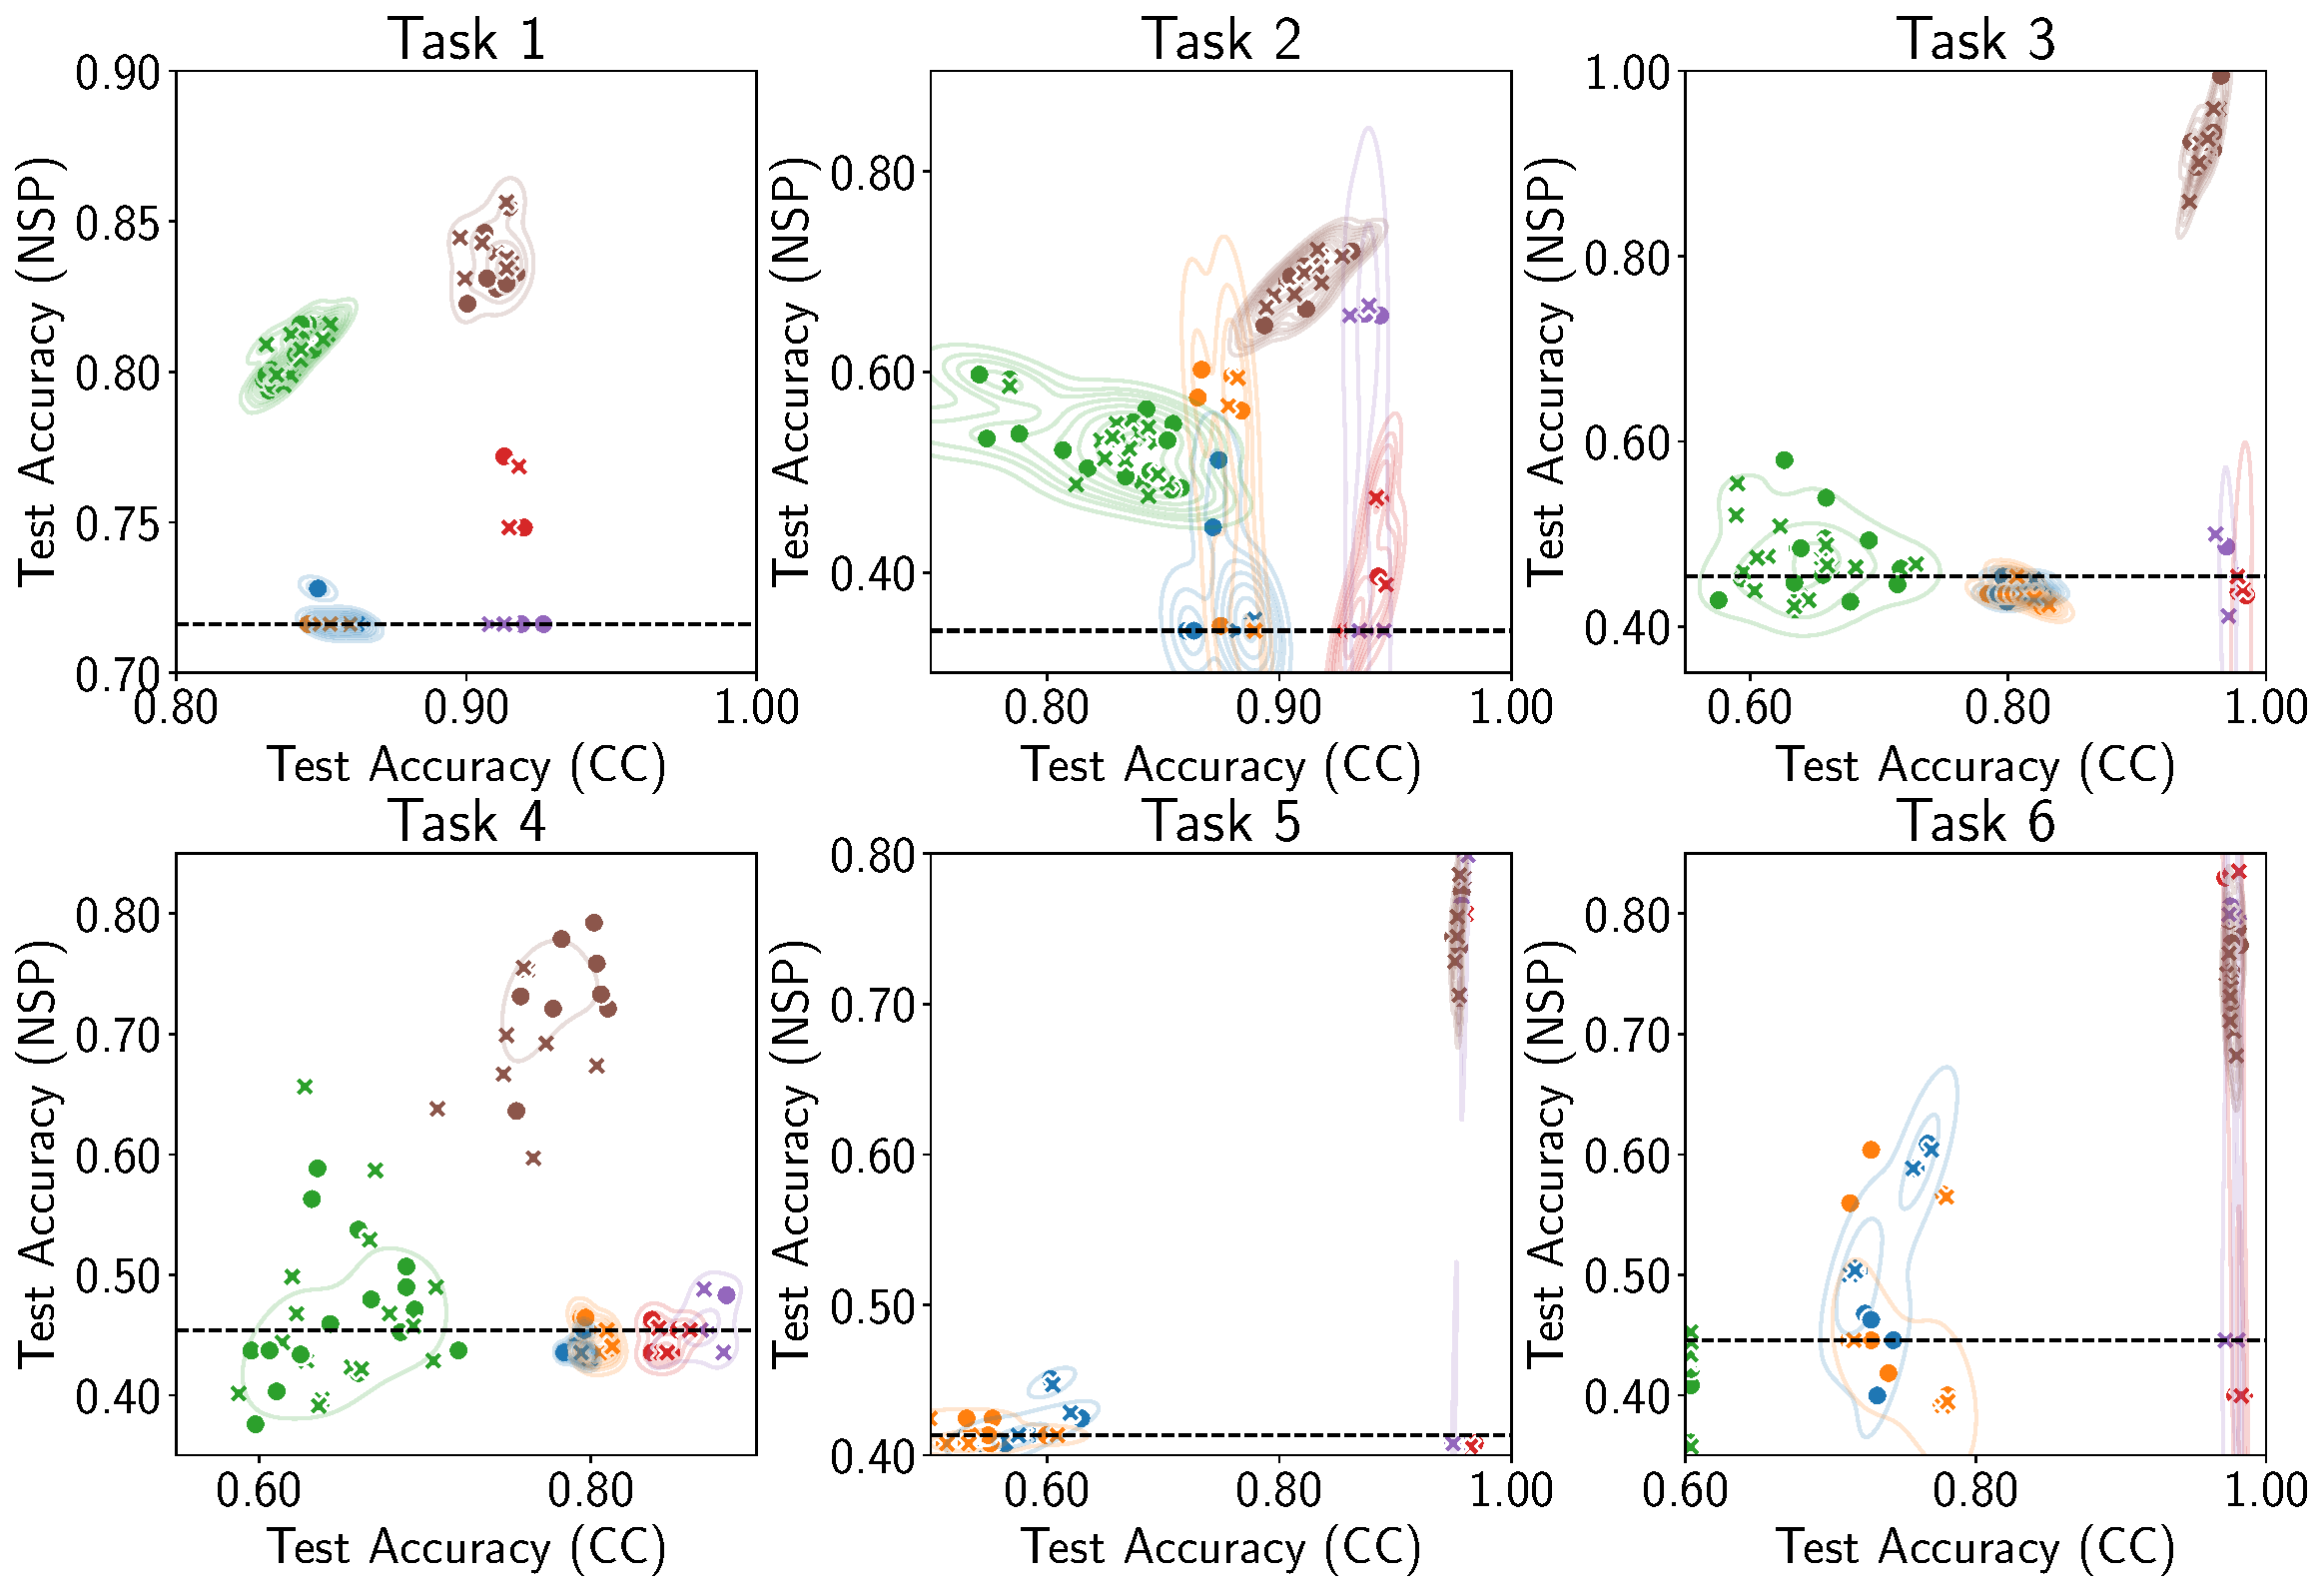
\includegraphics[width=1.0\textwidth]{imgs/ijcai/const-vs-succ.pdf}
	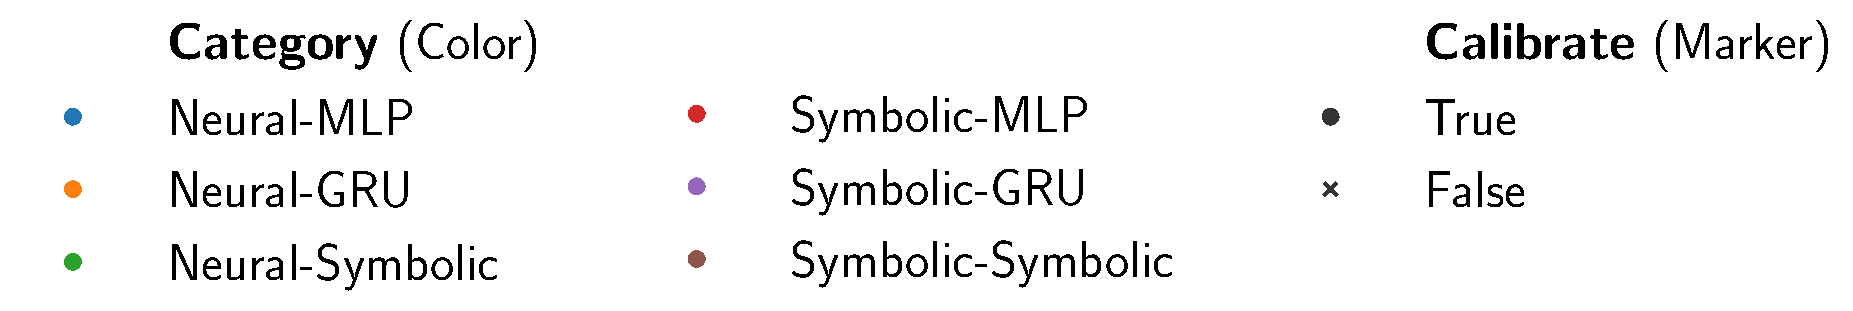
\includegraphics[width=1.0\textwidth]{imgs/ijcai/const-vs-succ_legend.pdf}
	\caption[{\sc cc}-{\sc nsp} accuracy trade-off on \textsc{LTLZinc-Sequential-Short-Legacy}]{{\sc cc}-{\sc nsp} accuracy trade-off on \textsc{LTLZinc-Sequential-Short-Legacy} for different families of architectures (i.e., Neural/Symbolic {\sc cc}, MLP/GRU/Symbolic {\sc nsp}). The dashed line indicates the baseline performance of a deterministic {\sc nsp} always selecting the state most represented in the training set. Axes stretched for readability.}
\label{ijcai:fig:main}
\end{figure*}
This experimental batch compares Neural vs. Neuro-symbolic methods on \textsc{LTLZinc-Sequential-Short-Legacy}, thus the effect of background knowledge over multiple reasoning steps, as well as the interaction between components.
We fix a neural perceptual backbone (\textsc{ic}), and then build four categories by combining either Neural (red blocks, Figure~\ref{ltlzinc:fig:pipeline}) or Symbolic (green, Figure~\ref{ltlzinc:fig:pipeline}) modules for constraint prediction (\textsc{cc}: MLP-S, MLP-L, Scallop) and temporal reasoning (\textsc{nsp}: MLP-S, MLP-L, GRU-S, GRU-L, Fuzzy-P, Fuzzy-LP, sd-DNNF-P, sd-DNNF-LP). %For brevity, we will omit the (always neural) perception module, and 
We will indicate each configuration with a shorthand notation, e.g., Symbolic-Neural means Symbolic \textsc{cc} and Neural \textsc{nsp} modules.
Training is performed in two steps: 5 pre-training epochs for the \textsc{ic} module, and then 20 epochs of training for the entire architecture. Overall, these experiments confront 96 combinations, across 6 tasks, each seeded 3 times.
%
As additional hyper-parameters, we explore the effect of temperature calibration (for the symbolic modules only) and the Semantic-based Regularization loss function proposed by Umili et al.~\cite{umili2023grounding}:
\begin{align*}
	\gL_{\textsc{SC}}(pred, labels) = &1 - \bigoplus pred\llbracket labels = 1 \rrbracket +\\
	& 1 - \prod pred \llbracket labels = 0 \rrbracket,
\end{align*}
where $\bigoplus$ is a left-associative reduction for the exclusive-or, computed as:
$$\texttt{a} \oplus \texttt{b} \doteq (a + b - a \cdot b) \cdot (1 - a \cdot b).$$

\paragraph{Results.}
%
Fig.~\ref{ijcai:fig:main} highlights the trade-offs between \textsc{cc} and \textsc{nsp}, as a function of the different Neural/Symbolic implementations on \textsc{LTLZinc-Sequential-Short-Legacy}.
%
Exploiting a symbolic component both for \textsc{cc} and \textsc{nsp} (Symbolic-Symbolic, brown points) allows to achieve the best trade-off for every task considered. Unlike other combinations, these approaches consistently outperform naive baselines which always return the most probable class observed in the training set, both for \textsc{nsp} (dashed horizontal line), and \textsc{cc} (not shown, outside the left boundary of plots).
%
The additional learning capacity provided by temperature calibration (dots vs. crosses) has an overall limited effect.
%
With the exception of tasks 1, 2 and 4, neural modules for \textsc{nsp} (clusters Symbolic-MLP/GRU and Neural-MLP/GRU, blue, orange, red and purple) achieve unsatisfactory performance, even when fed with highly-accurate symbolic \textsc{cc} predictions. These architectures, at times, perform on par with the most probable guessing baseline, and often below it.
%
Symbolic modules for \textsc{nsp} are characterized by a large dispersion, due to optimization challenges: this is especially true when exploiting neural \textsc{cc} modules (Neural-Symbolic, green), but it can also be observed in combination with symbolic \textsc{cc} modules (Symbolic-Symbolic, brown). Conversely, neural \textsc{nsp}, even though often showing unsatisfactory performance, is characterized by a much smaller inter-experiment variance.
%
%Comparing different tasks, it can be observed that tasks 1 and 2 can be solved by most combinations of modules (with fully neural approaches, blue and orange points, struggling the most), while both relational and temporal knowledge are crucial for every other task.
%
%
Table~\ref{ijcai:tab:main} summarizes performance for each task. %Experiments are replicated three times, to evaluate variance caused by different initialization.
%
Overall, the Symbolic-Symbolic category dominates over other groups, with the exception of Task 5, where it performs slightly worse than the Symbolic-Neural family. When observing constraint accuracy alone, a downstream Symbolic \textsc{nsp} module often negatively affects performance, with Task 4 presenting the highest delta between Symbolic-Symbolic and Symbolic-Neural.
Conversely, when focusing on next state prediction, an upstream Symbolic \textsc{cc} module is beneficial to a downstream Symbolic temporal reasoning module, however this clear-cut performance improvement is flipped when the \textsc{nsp} module is neural. This behavior hints at complex interactions between \textsc{cc} and \textsc{nsp} modules, where architectural choices bi-directionally affect both components.
%
%No clear trend in the effect of other hyper-parameters can be identified. 
Other hyper-parameters have negligible effect. 
Early stopping is almost always triggered near the end of training, hinting at a possibly incomplete convergence. Temperature calibration is often selected, but performance improvements are minor (cfr. with Fig. \ref{ijcai:fig:main}), and the semantic loss proposed by Umili et al.~\cite{umili2023grounding} is not significantly different than traditional binary cross-entropy in our setting.
%
Variances across three runs for each set of hyper-parameters are low. Comparing this observation with Figure~\ref{ijcai:fig:main} (which, instead, highlights hyper-parameter-based variance), it can be observed that convergence in multi-stage Neuro-symbolic Sequence Classification is heavily dependent on architectural choices, but relatively unaffected by parameter initialization.
%
Task 3 is an exception and it presents a failure case of the Symbolic-Symbolic family, due to training instability. When able to converge, however, it is the only approach capable of improving over random guessing for this task (we reported this sample result surrounding the model name with parentheses).


\section{Symbolic Error-propagation Experiments}
\begin{figure*}
	\centering
	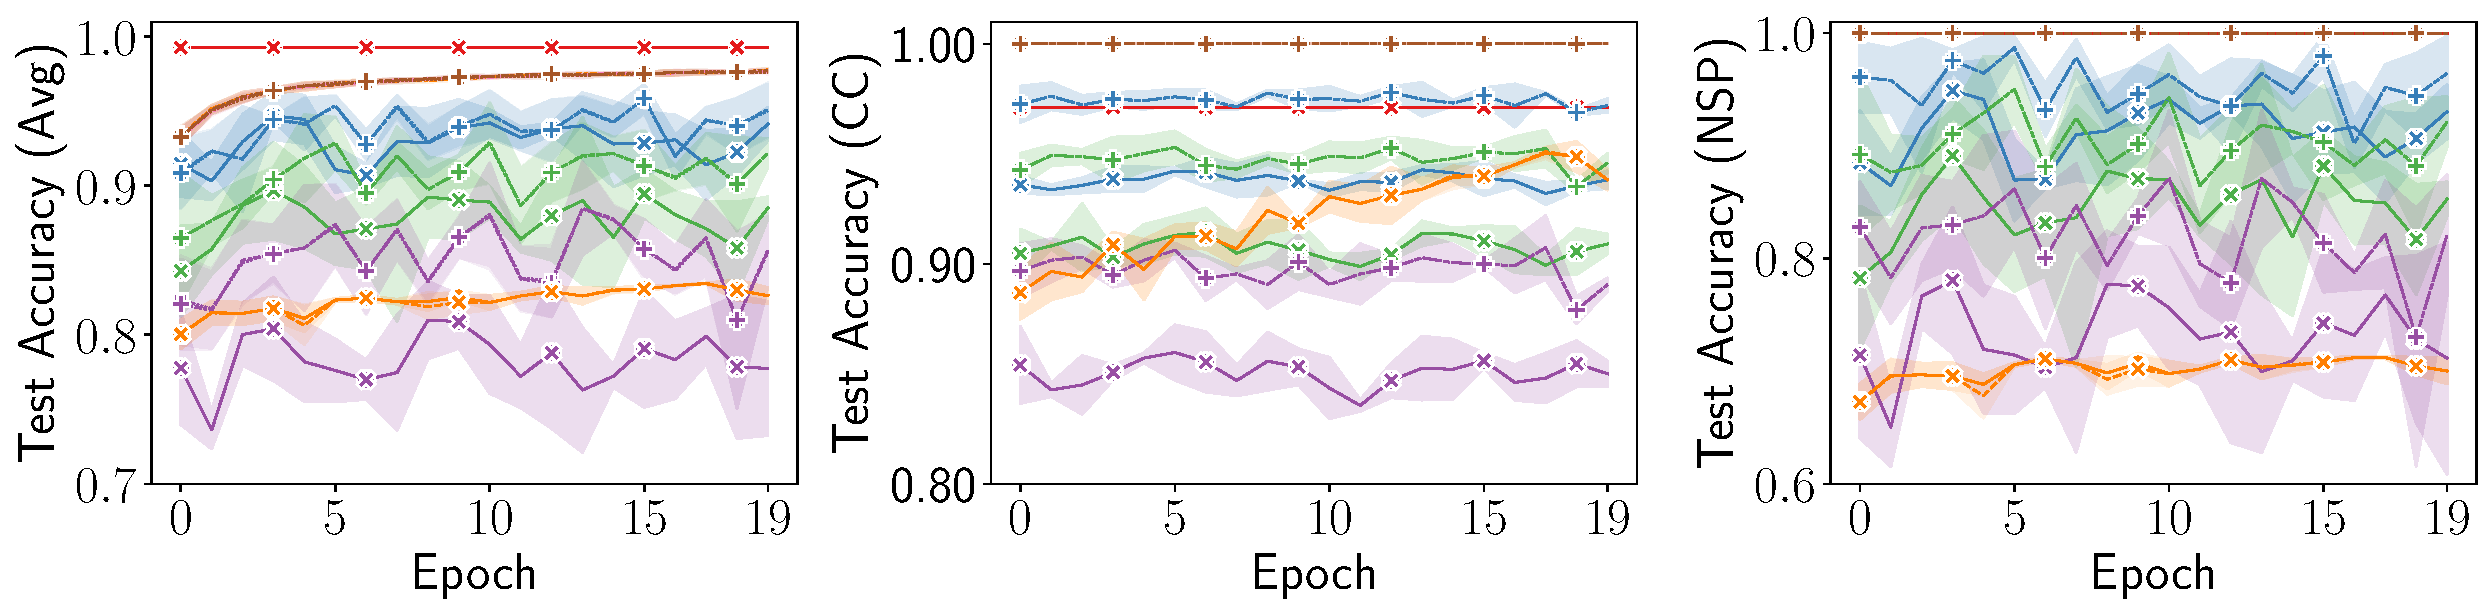
\includegraphics[width=\linewidth]{imgs/ijcai/ablation_task4.pdf}\\
	{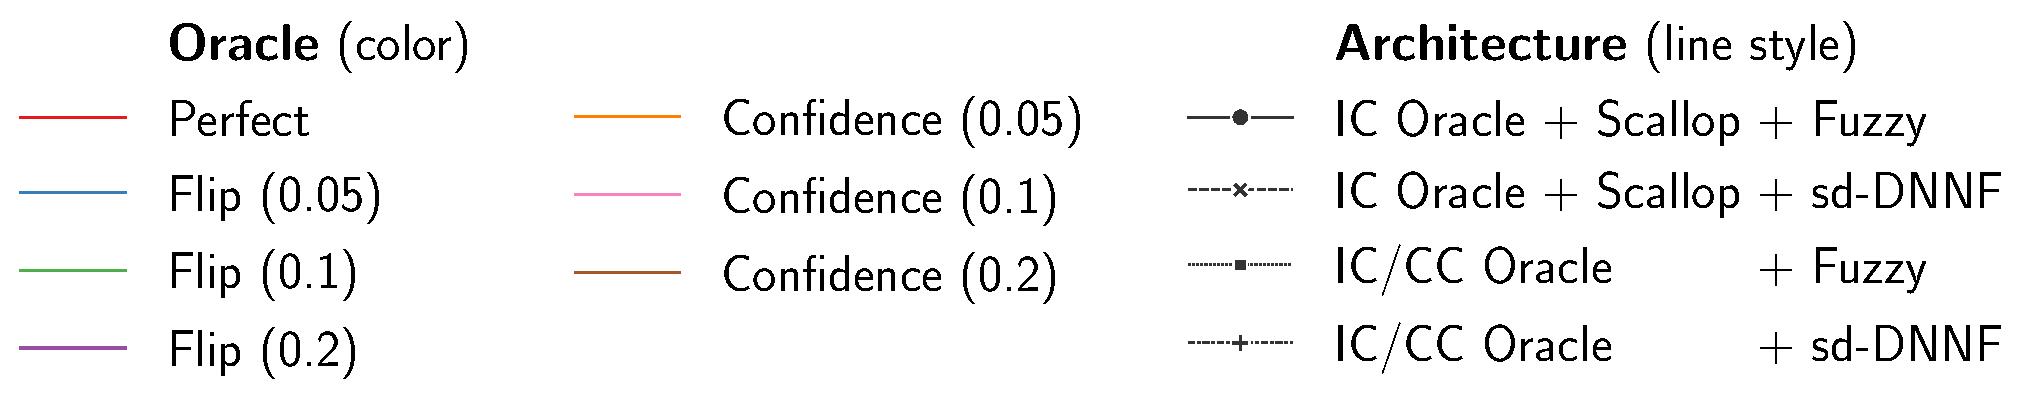
\includegraphics[width=\linewidth]{imgs/ijcai/ablation_task4_legend.pdf}}
	\caption[Error-propagation experiments on \textsc{LTLZinc-Sequential-Short-Legacy} (Task 4)]{Accuracies for \textsc{LTLZinc-Sequential-Short-Legacy} \textit{Task 4} with oracular predictors.}
	\label{ijcai:fig:abl-task4}
\end{figure*}

These experiments explicitly focus on the behavior of temporal reasoning modules, in a setting which more closely relates to traditional ``one-step'' Distant Supervision, exploring the effect of error propagation along Symbolic-Symbolic (green, Figure~\ref{ltlzinc:fig:pipeline}, \textsc{cc}: Scallop, \textsc{nsp}: Fuzzy-P, sd-DNNF-P) architectures.
We exploit probability calibration as the only form of learning, to minimize noise and precisely pinpoint the effect of variables such as upstream label uncertainty, and supervision ``distance'' from the reasoning component. We also consider replacing {\sc ic} and {\sc cc} modules with specific ``oracles'' returning the ground truth labels, possibly with some level of corruption. In particular, we either replace only \textsc{ic} (IC Oracle) or both \textsc{ic} and \textsc{cc} (IC/CC Oracle). %We will refer to the former case (an oracle for image labels followed by a Scallop program and then the temporal reasoning module under evaluation) as ``perceptual oracle'', and to the latter (an oracle for constraint labels followed by the temporal reasoning module under evaluation) as ``constraint oracle''.
%
An oracle is characterized by two hyper-parameters: how ground truth is corrupted before feeding the next module, and the amount of corruption in terms of noise probability $p$. ``Flip oracles'' return correct labels with probability $1-p$, and random labels with probability $p$, both with confidence $1.0$. ``Confidence oracles'', on the other hand, always return correct labels with random confidence between $1-p$ and $1.0$, redistributing the remaining mass to other labels.
When $p = 0.0$, both oracles yield ground truth labels with maximum confidence, referred to as ``perfect oracle''.
%We test $p \in [0.0, 0.05, 0.1, 0.2]$, for a total of 14 combinations of oracle distance, oracle nature and noise levels.



\paragraph{Results.}
Fig.~\ref{ijcai:fig:abl-task4} shows the effect on an exemplar task (Task 4) of oracular predictors on symbolic temporal reasoning modules.
Figures \ref{ijcai:fig:abl-avg}, \ref{ijcai:fig:abl-const} and \ref{ijcai:fig:abl-succ}, in Appendix~\ref{app:ltlzincoracle}, show the same plots for every task.
%
In general, the trainable temperature parameters are quickly optimized, with curves following a mostly horizontal trend. However, flip oracles (blue, green and purple lines) are characterized both by larger variance and inter-epoch oscillations, compared to confidence oracles (orange, pink and brown), which present a remarkably stable behavior. This effect is observed in every task, regardless of reasoning difficulty.
%
Noise injection, however, affects the two oracles differently: performance for flip oracles degrades linearly when increasing noise, while confidence oracles are characterized by non-linear behavior. Small amounts of noise do not affect confidence oracles appreciably, while larger amounts tend to harm performance more than the flip oracle. This effect is more evident for harder reasoning tasks: for instance, in Task 4, a noise of $p = 0.1$ is enough to cause random guessing performance (Figure~\ref{ijcai:fig:abl-task4-nolimits} in Appendix~\ref{app:ltlzincoracle}).
%
With oracles, the effect of different automata encodings is virtually non-existent (fuzzy and sd-DNNF markers overlap almost everywhere). 
%
\textsc{IC} oracles are consistently more affected by noise, compared to \textsc{IC/CC} ones. This behavior seems counterintuitive, as the Scallop module performs near-exact inference; however, it is in line with the hypothesis of uncertainty accumulation over multiple steps of reasoning.
%
When focusing on constraint performance (Figure~\ref{ijcai:fig:abl-const} in Appendix~\ref{app:ltlzincoracle}), flip oracles tend to have stable performance, while confidence oracles can exploit temperature parameters to achieve a small learning capacity (slight upward trend across epochs).
In general, flip oracles are more robust to noise, with confidence oracles achieving unsatisfactory performance (outside plot boundaries, Figure~\ref{ijcai:fig:abl-task4-nolimits} in Appendix~\ref{app:ltlzincoracle}) for harder tasks or higher ($p > 0.05$) degrees of uncertainty.
This behavior clashes with the desirable property of predictive confidence correlating with uncertainty, which is one of the advantages of Neuro-symbolic Artificial Intelligence, compared to (uncalibrated) Neural Networks. Flip oracles achieving better performance than confidence oracles, for similar levels of noise, hint at the fact that an overconfidently-wrong classifier can be more successful than a reluctantly-correct one, in temporal reasoning settings.
%
%Regarding performance on successor prediction (Fig. \ref{ijcai:fig:abl-succ}), the choice of automaton encoding does not play any role (solid and dotted, dashed and dot-dashed lines overlap each other for almost every data point), hinting at the fact that performance degradation due to upstream predictive noise is not affected by the presence of neutral and disjoint sum problems, however, as noted previously, a probabilistic semantics (sd-DNNF encoding) can be beneficial on upstream constraint prediction performance, possibly due to more stable gradients computed during backpropagation.
%
%The small positive slope identified in constraint prediction for confidence oracles does not propagate to next state prediction, where both flip and confidence oracles present an horizontal trend. At the same time, however, confidence oracles are characterized by a smoother training progression and lower inter-experiment variance, as it was the case for constraint prediction.


\section{Long-training Experiments}
In this section we explore the effect of varying sequence length, by comparing results on \textsc{LTLZinc-Sequential-Short} and \textsc{LTLZinc-Sequential-Long}. We explore the following combinations: Scallop (top-1 proof), ProbLog (exact inference), MLP-L (\textsc{cc}), and MLP-L, GRU-L, Fuzzy-P, sd-DNNF-P (\textsc{nsp}).
Temperature calibration is enabled for each symbolic module.
The \textsc{ic} module is pre-trained for 1 epoch and we explore the effect of additional training by varying the maximum number of epochs in $\{20, 50\}$.

\paragraph{Results.}
\begin{table}
	\centering
	\resizebox{\textwidth}{!}{
		\begin{tabular}{cccccccc}
			\toprule
			\multirow{2}{*}{\sc Task} & \multirow{2}{*}{\sc Category} & \multirow{2}{*}{\shortstack[c]{\sc Best model\\\sc (best epoch)}} & \multirow{2}{*}{\shortstack[c]{\sc Average\\\sc Accuracy}\raisebox{1ex}{\:$\uparrow$}} & \multirow{2}{*}{\shortstack[c]{\sc Label\\\sc Accuracy}\raisebox{1ex}{\:$\uparrow$}} & \multirow{2}{*}{\shortstack[c]{\sc Constraint\\\sc Accuracy}\raisebox{1ex}{\:$\uparrow$}} & \multirow{2}{*}{\shortstack[c]{\sc Successor\\\sc Accuracy}\raisebox{1ex}{\:$\uparrow$}} & \multirow{2}{*}{\shortstack[c]{\sc Sequence\\\sc Accuracy}\raisebox{1ex}{\:$\uparrow$}}\\
			& & & & & &\\
			\midrule
			\multirow{6}{*}{\shortstack[c]{Task 1}} & Sym. (exact)-Sym. & ProbLog sd-DNNF (49) & $0.69 $ {\tiny ($\pm 0.03$)} & $0.73 $ {\tiny ($\pm 0.09$)} & $\textbf{0.93} $ {\tiny ($\pm 0.01$)} & $0.61 $ {\tiny ($\pm 0.02$)} & $0.50 $ {\tiny ($\pm 0.00$)}\\
			& Sym. (exact)-Neu. & ProbLog GRU (47) & $\textbf{0.85} $ {\tiny ($\pm 0.00$)} & $\textbf{0.85} $ {\tiny ($\pm 0.00$)} & $0.92 $ {\tiny ($\pm 0.00$)} & $\textbf{0.72} $ {\tiny ($\pm 0.02$)} & $\textbf{0.93} $ {\tiny ($\pm 0.00$)}\\
			& Sym. (top-1)-Sym. & Scallop Fuzzy (49) & $0.70 $ {\tiny ($\pm 0.01$)} & $0.82 $ {\tiny ($\pm 0.06$)} & $0.92 $ {\tiny ($\pm 0.01$)} & $0.56 $ {\tiny ($\pm 0.00$)} & $0.50 $ {\tiny ($\pm 0.00$)}\\
			& Sym. (top-1)-Neu. & Scallop MLP (46) & $0.84 $ {\tiny ($\pm 0.01$)} & $\textbf{0.85} $ {\tiny ($\pm 0.01$)} & $0.90 $ {\tiny ($\pm 0.00$)} & $0.70 $ {\tiny ($\pm 0.03$)} & $0.92 $ {\tiny ($\pm 0.01$)}\\
			& Neu.-Sym. & MLP Fuzzy (48) & $0.70 $ {\tiny ($\pm 0.01$)} & $\textbf{0.85} $ {\tiny ($\pm 0.01$)} & $0.90 $ {\tiny ($\pm 0.01$)} & $0.55 $ {\tiny ($\pm 0.02$)} & $0.50 $ {\tiny ($\pm 0.00$)}\\
			& Neu.-Neu. & MLP MLP (42) & $0.82 $ {\tiny ($\pm 0.04$)} & $0.81 $ {\tiny ($\pm 0.06$)} & $0.88 $ {\tiny ($\pm 0.03$)} & $0.69 $ {\tiny ($\pm 0.05$)} & $0.91 $ {\tiny ($\pm 0.01$)}\\
			\hdashline
			\multirow{6}{*}{\shortstack[c]{Task 2}} & Sym. (exact)-Sym. & ProbLog Fuzzy (49) & $0.79 $ {\tiny ($\pm 0.03$)} & $0.84 $ {\tiny ($\pm 0.06$)} & $0.92 $ {\tiny ($\pm 0.02$)} & $0.66 $ {\tiny ($\pm 0.01$)} & $0.72 $ {\tiny ($\pm 0.04$)}\\
			& Sym. (exact)-Neu. & ProbLog GRU (30) & $\textbf{0.89} $ {\tiny ($\pm 0.01$)} & $0.87 $ {\tiny ($\pm 0.00$)} & $0.91 $ {\tiny ($\pm 0.00$)} & $0.83 $ {\tiny ($\pm 0.02$)} & $\textbf{0.96} $ {\tiny ($\pm 0.02$)}\\
			& Sym. (top-1)-Sym. & Scallop sd-DNNF (49) & $0.79 $ {\tiny ($\pm 0.01$)} & $\textbf{0.90} $ {\tiny ($\pm 0.00$)} & $\textbf{0.93} $ {\tiny ($\pm 0.00$)} & $0.63 $ {\tiny ($\pm 0.02$)} & $0.71 $ {\tiny ($\pm 0.01$)}\\
			& Sym. (top-1)-Neu. & Scallop MLP (46) & $0.88 $ {\tiny ($\pm 0.00$)} & $0.87 $ {\tiny ($\pm 0.00$)} & $0.92 $ {\tiny ($\pm 0.00$)} & $\textbf{0.85} $ {\tiny ($\pm 0.00$)} & $0.88 $ {\tiny ($\pm 0.00$)}\\
			& Neu.-Sym. & MLP Fuzzy (46) & $0.79 $ {\tiny ($\pm 0.01$)} & $0.86 $ {\tiny ($\pm 0.01$)} & $0.88 $ {\tiny ($\pm 0.01$)} & $0.67 $ {\tiny ($\pm 0.01$)} & $0.74 $ {\tiny ($\pm 0.03$)}\\
			& Neu.-Neu. & MLP GRU (47) & $0.86 $ {\tiny ($\pm 0.01$)} & $0.86 $ {\tiny ($\pm 0.01$)} & $0.90 $ {\tiny ($\pm 0.01$)} & $0.81 $ {\tiny ($\pm 0.01$)} & $0.88 $ {\tiny ($\pm 0.07$)}\\
			\hdashline
			\multirow{6}{*}{\shortstack[c]{Task 3}} & Sym. (exact)-Sym. & ProbLog Fuzzy (48) & $\textbf{0.96} $ {\tiny ($\pm 0.00$)} & $0.97 $ {\tiny ($\pm 0.00$)} & $0.97 $ {\tiny ($\pm 0.00$)} & $0.94 $ {\tiny ($\pm 0.00$)} & $\textbf{0.95} $ {\tiny ($\pm 0.00$)}\\
			& Sym. (exact)-Neu. & ProbLog MLP (42) & $0.74 $ {\tiny ($\pm 0.01$)} & $\textbf{0.99} $ {\tiny ($\pm 0.00$)} & $\textbf{0.99} $ {\tiny ($\pm 0.00$)} & $0.56 $ {\tiny ($\pm 0.03$)} & $0.41 $ {\tiny ($\pm 0.01$)}\\
			& Sym. (top-1)-Sym. & Scallop sd-DNNF (43) & $\textbf{0.96} $ {\tiny ($\pm 0.00$)} & $0.96 $ {\tiny ($\pm 0.00$)} & $0.97 $ {\tiny ($\pm 0.01$)} & $\textbf{0.95} $ {\tiny ($\pm 0.00$)} & $\textbf{0.95} $ {\tiny ($\pm 0.00$)}\\
			& Sym. (top-1)-Neu. & Scallop MLP (48) & $0.75 $ {\tiny ($\pm 0.01$)} & $0.98 $ {\tiny ($\pm 0.00$)} & $0.98 $ {\tiny ($\pm 0.00$)} & $0.59 $ {\tiny ($\pm 0.02$)} & $0.45 $ {\tiny ($\pm 0.05$)}\\
			& Neu.-Sym. & MLP Fuzzy (29) & $0.78 $ {\tiny ($\pm 0.01$)} & $0.93 $ {\tiny ($\pm 0.02$)} & $0.79 $ {\tiny ($\pm 0.01$)} & $0.71 $ {\tiny ($\pm 0.03$)} & $0.69 $ {\tiny ($\pm 0.03$)}\\
			& Neu.-Neu. & MLP MLP (47) & $0.72 $ {\tiny ($\pm 0.01$)} & $\textbf{0.99} $ {\tiny ($\pm 0.00$)} & $0.91 $ {\tiny ($\pm 0.01$)} & $0.54 $ {\tiny ($\pm 0.02$)} & $0.45 $ {\tiny ($\pm 0.05$)}\\
			\hdashline
			\multirow{6}{*}{\shortstack[c]{Task 4}} & Sym. (exact)-Sym. & ProbLog sd-DNNF (37) & $0.87 $ {\tiny ($\pm 0.02$)} & $0.86 $ {\tiny ($\pm 0.01$)} & $0.89 $ {\tiny ($\pm 0.01$)} & $0.88 $ {\tiny ($\pm 0.04$)} & $0.87 $ {\tiny ($\pm 0.04$)}\\
			& Sym. (exact)-Neu. & ProbLog MLP (46) & $0.72 $ {\tiny ($\pm 0.02$)} & $\textbf{0.91} $ {\tiny ($\pm 0.00$)} & $\textbf{0.93} $ {\tiny ($\pm 0.00$)} & $0.58 $ {\tiny ($\pm 0.01$)} & $0.47 $ {\tiny ($\pm 0.08$)}\\
			& Sym. (top-1)-Sym. & Scallop sd-DNNF (50) & $\textbf{0.88} $ {\tiny ($\pm 0.01$)} & $0.86 $ {\tiny ($\pm 0.01$)} & $0.84 $ {\tiny ($\pm 0.01$)} & $\textbf{0.90} $ {\tiny ($\pm 0.02$)} & $\textbf{0.90} $ {\tiny ($\pm 0.03$)}\\
			& Sym. (top-1)-Neu. & Scallop MLP (41) & $0.72 $ {\tiny ($\pm 0.00$)} & $\textbf{0.91} $ {\tiny ($\pm 0.01$)} & $0.89 $ {\tiny ($\pm 0.00$)} & $0.55 $ {\tiny ($\pm 0.03$)} & $0.52 $ {\tiny ($\pm 0.01$)}\\
			& Neu.-Sym. & MLP Fuzzy (47) & $0.71 $ {\tiny ($\pm 0.01$)} & $0.83 $ {\tiny ($\pm 0.02$)} & $0.72 $ {\tiny ($\pm 0.03$)} & $0.67 $ {\tiny ($\pm 0.04$)} & $0.62 $ {\tiny ($\pm 0.04$)}\\
			& Neu.-Neu. & MLP MLP (46) & $0.70 $ {\tiny ($\pm 0.02$)} & $\textbf{0.91} $ {\tiny ($\pm 0.01$)} & $0.87 $ {\tiny ($\pm 0.01$)} & $0.55 $ {\tiny ($\pm 0.01$)} & $0.47 $ {\tiny ($\pm 0.07$)}\\
			\hdashline
			\multirow{6}{*}{\shortstack[c]{Task 5}} & Sym. (exact)-Sym. & ProbLog sd-DNNF (19) & $0.53 $ {\tiny ($\pm 0.31$)} & $0.40 $ {\tiny ($\pm 0.51$)} & $0.71 $ {\tiny ($\pm 0.23$)} & $0.41 $ {\tiny ($\pm 0.36$)} & $0.59 $ {\tiny ($\pm 0.16$)}\\
			& Sym. (exact)-Neu. & ProbLog MLP (39) & $0.96 $ {\tiny ($\pm 0.01$)} & $0.98 $ {\tiny ($\pm 0.00$)} & $0.96 $ {\tiny ($\pm 0.00$)} & $0.94 $ {\tiny ($\pm 0.00$)} & $\textbf{0.98} $ {\tiny ($\pm 0.03$)}\\
			& Sym. (top-1)-Sym. & Scallop Fuzzy (44) & $0.51 $ {\tiny ($\pm 0.34$)} & $0.40 $ {\tiny ($\pm 0.51$)} & $0.64 $ {\tiny ($\pm 0.29$)} & $0.41 $ {\tiny ($\pm 0.38$)} & $0.60 $ {\tiny ($\pm 0.17$)}\\
			& Sym. (top-1)-Neu. & Scallop MLP (48) & $\textbf{0.98} $ {\tiny ($\pm 0.00$)} & $\textbf{0.99} $ {\tiny ($\pm 0.00$)} & $\textbf{0.97} $ {\tiny ($\pm 0.00$)} & $\textbf{0.98} $ {\tiny ($\pm 0.00$)} & $\textbf{0.98} $ {\tiny ($\pm 0.00$)}\\
			& Neu.-Sym. & MLP sd-DNNF (49) & $0.62 $ {\tiny ($\pm 0.01$)} & $0.94 $ {\tiny ($\pm 0.02$)} & $0.75 $ {\tiny ($\pm 0.02$)} & $0.28 $ {\tiny ($\pm 0.01$)} & $0.50 $ {\tiny ($\pm 0.00$)}\\
			& Neu.-Neu. & MLP MLP (47) & $0.80 $ {\tiny ($\pm 0.03$)} & $0.93 $ {\tiny ($\pm 0.04$)} & $0.71 $ {\tiny ($\pm 0.04$)} & $0.77 $ {\tiny ($\pm 0.01$)} & $0.80 $ {\tiny ($\pm 0.03$)}\\
			\hdashline
			\multirow{6}{*}{\shortstack[c]{Task 6}} & Sym. (exact)-Sym. & ProbLog sd-DNNF (46) & $0.60 $ {\tiny ($\pm 0.00$)} & $\textbf{0.99} $ {\tiny ($\pm 0.00$)} & $0.53 $ {\tiny ($\pm 0.00$)} & $0.38 $ {\tiny ($\pm 0.00$)} & $0.50 $ {\tiny ($\pm 0.00$)}\\
			& Sym. (exact)-Neu. & ProbLog GRU (49) & $0.62 $ {\tiny ($\pm 0.01$)} & $\textbf{0.99} $ {\tiny ($\pm 0.00$)} & $0.53 $ {\tiny ($\pm 0.00$)} & $0.44 $ {\tiny ($\pm 0.03$)} & $0.50 $ {\tiny ($\pm 0.00$)}\\
			& Sym. (top-1)-Sym. & Scallop sd-DNNF (50) & $0.74 $ {\tiny ($\pm 0.04$)} & $0.97 $ {\tiny ($\pm 0.01$)} & $\textbf{0.96} $ {\tiny ($\pm 0.01$)} & $0.50 $ {\tiny ($\pm 0.12$)} & $0.52 $ {\tiny ($\pm 0.03$)}\\
			& Sym. (top-1)-Neu. & Scallop MLP (48) & $\textbf{0.91} $ {\tiny ($\pm 0.03$)} & $0.97 $ {\tiny ($\pm 0.02$)} & $\textbf{0.96} $ {\tiny ($\pm 0.02$)} & $\textbf{0.88} $ {\tiny ($\pm 0.04$)} & $\textbf{0.83} $ {\tiny ($\pm 0.04$)}\\
			& Neu.-Sym. & MLP Fuzzy (50) & $0.64 $ {\tiny ($\pm 0.06$)} & $0.97 $ {\tiny ($\pm 0.01$)} & $0.79 $ {\tiny ($\pm 0.17$)} & $0.29 $ {\tiny ($\pm 0.09$)} & $0.50 $ {\tiny ($\pm 0.00$)}\\
			& Neu.-Neu. & MLP MLP (49) & $0.86 $ {\tiny ($\pm 0.03$)} & $0.98 $ {\tiny ($\pm 0.00$)} & $0.91 $ {\tiny ($\pm 0.01$)} & $0.82 $ {\tiny ($\pm 0.03$)} & $0.73 $ {\tiny ($\pm 0.06$)}\\
			\bottomrule
		\end{tabular}
	}
	\caption[Test set accuracies on \textsc{LTLZinc-Sequential-Short}]{Best models test set accuracies (mean $\pm$ std over 3 random seeds, after discarding diverging runs) for \textsc{LTLZinc-Sequential-Short} experiments, grouped by category. Best model (named ``{\sc cc} model {\sc nsp} model'') and epoch selected by \textsc{Average Accuracy} on validation set.}
	\label{ltlzinc:tab:sequential-results-short}
\end{table}
%
Table~\ref{ltlzinc:tab:sequential-results-short} summarizes the best results on \textsc{LTLZinc-Sequential-Short} for every task. One result immediately observable from the table is that purely neural approaches are insufficient to adequately capture the complex nature of the tasks. Though in some cases the label accuracy matches that of neural-symbolic or symbolic-symbolic approaches (e.g., in \textsc{Task 3}), overall the performance is much worse, especially for successor accuracy and the final task of sequence classification. As for the other approaches, there is no clear class of winner methods for each and every task, though the approach that combines Scallop with top-1 proof for constraint classification with a Multi-Layer Perceptron for next state prediction seems to be a reasonable compromise across multiple tasks.
%
For a more detailed analysis of these results, Figure~\ref{ltlzinc:fig:sequential-tradeoff-short} shows, for every short-sequence experimental run, the \textsc{cc}-\textsc{nsp} accuracy trade-off, highlighting different characteristics of each category. These results strongly confirm the advantages of Symbolic-Symbolic, or Neural-Symbolic, approaches with respect to purely neural architectures, even though they are harder to optimize (larger dispersion between points, compared to neural-only approaches, and fewer data points available due to diverging runs). The scatter plots also highlight the contribution of training epochs: more epochs, in fact, seem to help the system achieving an overall better performance (in the charts, this is indicated by dots closer to the top-right corner with respect to crosses, regardless of color), even though some families benefit less from additional training.
%
\begin{figure}
	\centering
	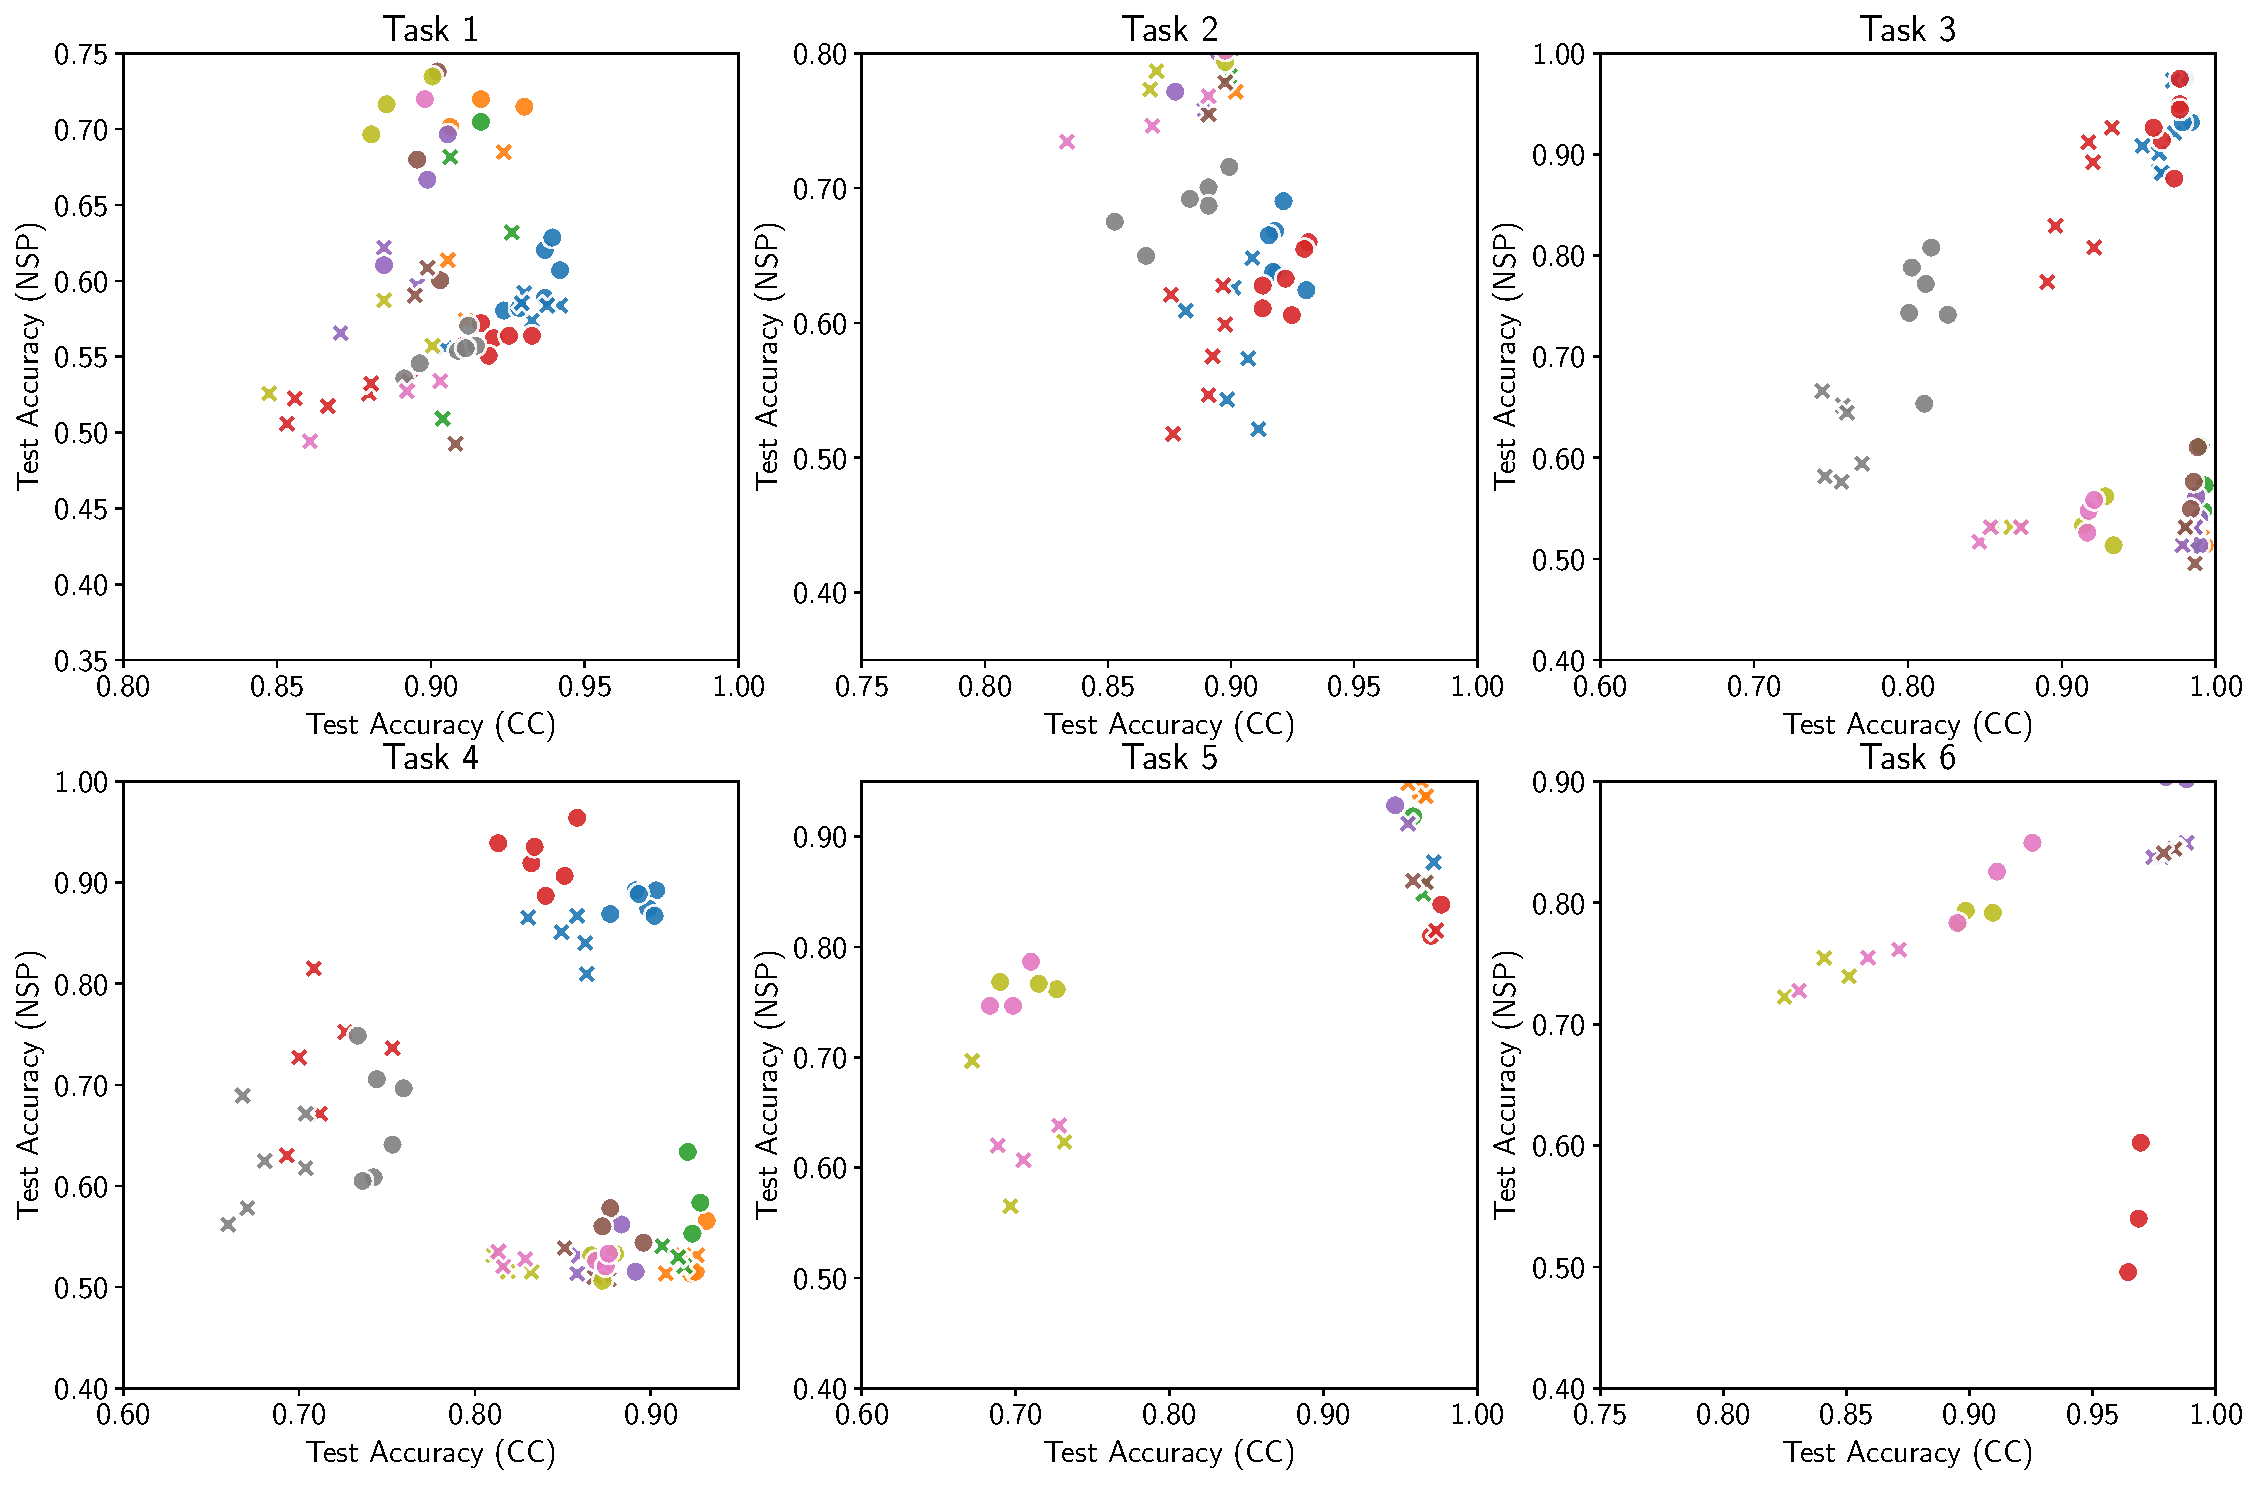
\includegraphics[width=1.0\textwidth]{imgs/ltlzinc/const-vs-succ-short.pdf}
	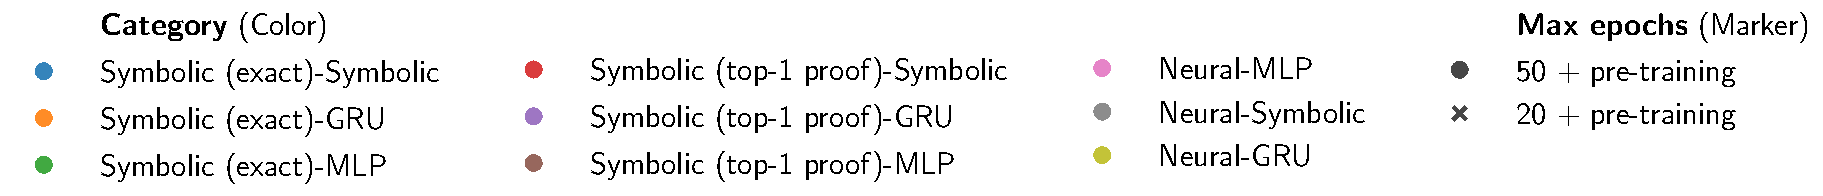
\includegraphics[width=1.0\textwidth]{imgs/ltlzinc/const-vs-succ_legend.pdf}
	\caption[\textsc{cc}--\textsc{nsp} accuracy trade-off on \textsc{LTLZinc-Sequential-Short}]{{\sc cc}-{\sc nsp} accuracy trade-off on \textsc{LTLZinc-Sequential-Short} experiments for different categories.} %Axes stretched for readability.}
\label{ltlzinc:fig:sequential-tradeoff-short}
\end{figure}
%
Focusing on symbolic methods for \textsc{cc} and \textsc{nsp} (red for Scallop and Deterministic Finite-state Automata, blue for ProbLog and Deterministic Finite-state Automata), they generally achieve similar performances, but with some trends identifiable in specific tasks. For tasks 1-4, a symbolic Scallop module is characterized by a noticeable dependency on the number of training epochs (red crosses and red dots forming two distinct clusters), while ProbLog, under the same tasks, can achieve similar performance (clusters can still be identified, with 50 epochs being slightly better, but they lie very close to each other), regardless of the number of training epochs. This behavior can in part be explained by the amount of information back-propagated through either component (only along the most probable proof for Scallop, and along the entire proof-tree for ProbLog). Tasks 5 and 6 pose optimization challenges for both methods, with only few combinations of hyper-parameters able to converge (a zero variance in Table~\ref{ltlzinc:tab:sequential-results-short} is often due to only one experiment being able to converge).
%
Table~\ref{ltlzinc:tab:sequential-results-long} corresponds to experiments on \textsc{LTLZinc-Sequential-Long}. Neural-only experiments do not benefit from longer sequence horizons, as their accuracies across every objective remain roughly the same. Regardless of the \textsc{cc} module, label and constraint accuracies are also close to their short-sequence experiment counterparts. This result is somewhat expected, as neither objective is time dependent. The additional amount of data (about 5 to 10 times more abundant when moving from sequences of random length 10-20 to sequences of random length 50-100) does not seem to provide noticeable benefits in terms of label or constraint accuracy.
When focusing on \textsc{nsp} and \textsc{sc} objectives, it can be observed an improvement of performance, compared to short-sequence experiments, but only for those combinations which already managed to achieve good performance. The gap between good and bad combinations is noticeably increased, with sequence accuracy basically being either close to random guessing, or close to perfect classification.
\begin{table}
\centering
\resizebox{\textwidth}{!}{
	\begin{tabular}{cccccccc}
		\toprule
		\multirow{2}{*}{\sc Task} & \multirow{2}{*}{\sc Category} & \multirow{2}{*}{\shortstack[c]{\sc Best model\\\sc (best epoch)}} & \multirow{2}{*}{\shortstack[c]{\sc Average\\\sc Accuracy}\raisebox{1ex}{\:$\uparrow$}} & \multirow{2}{*}{\shortstack[c]{\sc Label\\\sc Accuracy}\raisebox{1ex}{\:$\uparrow$}} & \multirow{2}{*}{\shortstack[c]{\sc Constraint\\\sc Accuracy}\raisebox{1ex}{\:$\uparrow$}} & \multirow{2}{*}{\shortstack[c]{\sc Successor\\\sc Accuracy}\raisebox{1ex}{\:$\uparrow$}} & \multirow{2}{*}{\shortstack[c]{\sc Sequence\\\sc Accuracy}\raisebox{1ex}{\:$\uparrow$}}\\
		& & & & & &\\
		\midrule
		\multirow{6}{*}{\shortstack[c]{Task 1\\(long)}} & Sym. (exact)-Sym. & ProbLog Fuzzy (45) & $0.69 $ {\tiny ($\pm 0.00$)} & $0.81 $ {\tiny ($\pm 0.00$)} & $\textbf{0.94} $ {\tiny ($\pm 0.00$)} & $0.52 $ {\tiny ($\pm 0.00$)} & $0.50 $ {\tiny ($\pm 0.00$)}\\
		& Sym. (exact)-Neu. & ProbLog MLP (43) & $\textbf{0.90} $ {\tiny ($\pm 0.01$)} & $\textbf{0.87} $ {\tiny ($\pm 0.02$)} & $0.92 $ {\tiny ($\pm 0.02$)} & $\textbf{0.83} $ {\tiny ($\pm 0.02$)} & $\textbf{1.00} $ {\tiny ($\pm 0.00$)}\\
		& Sym. (top-1)-Sym. & Scallop sd-DNNF (50) & $0.69 $ {\tiny ($\pm 0.00$)} & $0.83 $ {\tiny ($\pm 0.04$)} & $0.92 $ {\tiny ($\pm 0.02$)} & $0.51 $ {\tiny ($\pm 0.00$)} & $0.50 $ {\tiny ($\pm 0.00$)}\\
		& Sym. (top-1)-Neu. & Scallop MLP (40) & $0.87 $ {\tiny ($\pm 0.01$)} & $0.85 $ {\tiny ($\pm 0.03$)} & $0.90 $ {\tiny ($\pm 0.01$)} & $0.77 $ {\tiny ($\pm 0.00$)} & $0.96 $ {\tiny ($\pm 0.02$)}\\
		& Neu.-Sym. & MLP sd-DNNF (50) & $0.68 $ {\tiny ($\pm 0.03$)} & $0.88 $ {\tiny ($\pm 0.01$)} & $0.85 $ {\tiny ($\pm 0.12$)} & $0.50 $ {\tiny ($\pm 0.02$)} & $0.50 $ {\tiny ($\pm 0.00$)}\\
		& Neu.-Neu. & MLP GRU (47) & $0.80 $ {\tiny ($\pm 0.11$)} & $0.83 $ {\tiny ($\pm 0.03$)} & $0.88 $ {\tiny ($\pm 0.02$)} & $0.62 $ {\tiny ($\pm 0.26$)} & $0.88 $ {\tiny ($\pm 0.16$)}\\
		\hdashline
		\multirow{6}{*}{\shortstack[c]{Task 2\\(long)}} & Sym. (exact)-Sym. & ProbLog Fuzzy (49) & $0.64 $ {\tiny ($\pm 0.03$)} & $0.67 $ {\tiny ($\pm 0.12$)} & $0.92 $ {\tiny ($\pm 0.01$)} & $0.42 $ {\tiny ($\pm 0.02$)} & $0.54 $ {\tiny ($\pm 0.01$)}\\
		& Sym. (exact)-Neu. & ProbLog GRU (43) & $\textbf{0.85} $ {\tiny ($\pm 0.00$)} & $0.89 $ {\tiny ($\pm 0.01$)} & $\textbf{0.94} $ {\tiny ($\pm 0.00$)} & $\textbf{0.78} $ {\tiny ($\pm 0.00$)} & $\textbf{0.80} $ {\tiny ($\pm 0.00$)}\\
		& Sym. (top-1)-Sym. & Scallop Fuzzy (45) & $0.72 $ {\tiny ($\pm 0.02$)} & $\textbf{0.91} $ {\tiny ($\pm 0.01$)} & $0.93 $ {\tiny ($\pm 0.00$)} & $0.45 $ {\tiny ($\pm 0.01$)} & $0.57 $ {\tiny ($\pm 0.08$)}\\
		& Sym. (top-1)-Neu. & Scallop MLP (50) & $\textbf{0.85} $ {\tiny ($\pm 0.01$)} & $0.89 $ {\tiny ($\pm 0.02$)} & $0.93 $ {\tiny ($\pm 0.01$)} & $\textbf{0.78} $ {\tiny ($\pm 0.01$)} & $\textbf{0.80} $ {\tiny ($\pm 0.00$)}\\
		& Neu.-Sym. & MLP Fuzzy (45) & $0.70 $ {\tiny ($\pm 0.06$)} & $0.89 $ {\tiny ($\pm 0.01$)} & $0.85 $ {\tiny ($\pm 0.07$)} & $0.46 $ {\tiny ($\pm 0.08$)} & $0.58 $ {\tiny ($\pm 0.08$)}\\
		& Neu.-Neu. & MLP MLP (50) & $0.84 $ {\tiny ($\pm 0.00$)} & $0.89 $ {\tiny ($\pm 0.00$)} & $0.92 $ {\tiny ($\pm 0.00$)} & $0.76 $ {\tiny ($\pm 0.00$)} & $0.77 $ {\tiny ($\pm 0.00$)}\\
		\hdashline
		\multirow{6}{*}{\shortstack[c]{Task 3\\(long)}} & Sym. (exact)-Sym. & ProbLog sd-DNNF (46) & $\textbf{0.97} $ {\tiny ($\pm 0.00$)} & $0.98 $ {\tiny ($\pm 0.00$)} & $0.98 $ {\tiny ($\pm 0.00$)} & $\textbf{0.96} $ {\tiny ($\pm 0.00$)} & $0.95 $ {\tiny ($\pm 0.00$)}\\
		& Sym. (exact)-Neu. & ProbLog MLP (42) & $0.75 $ {\tiny ($\pm 0.01$)} & $\textbf{0.99} $ {\tiny ($\pm 0.00$)} & $\textbf{0.99} $ {\tiny ($\pm 0.00$)} & $0.50 $ {\tiny ($\pm 0.02$)} & $0.52 $ {\tiny ($\pm 0.03$)}\\
		& Sym. (top-1)-Sym. & Scallop Fuzzy (45) & $0.96 $ {\tiny ($\pm 0.01$)} & $0.97 $ {\tiny ($\pm 0.00$)} & $0.97 $ {\tiny ($\pm 0.00$)} & $\textbf{0.96} $ {\tiny ($\pm 0.01$)} & $\textbf{0.96} $ {\tiny ($\pm 0.01$)}\\
		& Sym. (top-1)-Neu. & Scallop MLP (43) & $0.75 $ {\tiny ($\pm 0.01$)} & $\textbf{0.99} $ {\tiny ($\pm 0.00$)} & $\textbf{0.99} $ {\tiny ($\pm 0.00$)} & $0.50 $ {\tiny ($\pm 0.02$)} & $0.51 $ {\tiny ($\pm 0.02$)}\\
		& Neu.-Sym. & MLP sd-DNNF (40) & $0.81 $ {\tiny ($\pm 0.01$)} & $0.93 $ {\tiny ($\pm 0.01$)} & $0.80 $ {\tiny ($\pm 0.02$)} & $0.76 $ {\tiny ($\pm 0.04$)} & $0.76 $ {\tiny ($\pm 0.03$)}\\
		& Neu.-Neu. & MLP MLP (20) & $0.72 $ {\tiny ($\pm 0.01$)} & $0.98 $ {\tiny ($\pm 0.00$)} & $0.90 $ {\tiny ($\pm 0.01$)} & $0.51 $ {\tiny ($\pm 0.01$)} & $0.49 $ {\tiny ($\pm 0.05$)}\\
		\hdashline
		\multirow{6}{*}{\shortstack[c]{Task 4\\(long)}} & Sym. (exact)-Sym. & ProbLog sd-DNNF (16) & $\textbf{0.86} $ {\tiny ($\pm 0.01$)} & $0.86 $ {\tiny ($\pm 0.00$)} & $0.89 $ {\tiny ($\pm 0.00$)} & $\textbf{0.84} $ {\tiny ($\pm 0.02$)} & $\textbf{0.84} $ {\tiny ($\pm 0.02$)}\\
		& Sym. (exact)-Neu. & ProbLog MLP (23) & $0.73 $ {\tiny ($\pm 0.01$)} & $0.91 $ {\tiny ($\pm 0.01$)} & $\textbf{0.92} $ {\tiny ($\pm 0.00$)} & $0.53 $ {\tiny ($\pm 0.01$)} & $0.54 $ {\tiny ($\pm 0.04$)}\\
		& Sym. (top-1)-Sym. & Scallop Fuzzy (18) & $0.79 $ {\tiny ($\pm 0.02$)} & $0.82 $ {\tiny ($\pm 0.03$)} & $0.80 $ {\tiny ($\pm 0.01$)} & $0.77 $ {\tiny ($\pm 0.04$)} & $0.78 $ {\tiny ($\pm 0.03$)}\\
		& Sym. (top-1)-Neu. & Scallop MLP (49) & $0.71 $ {\tiny ($\pm 0.01$)} & $\textbf{0.92} $ {\tiny ($\pm 0.01$)} & $0.91 $ {\tiny ($\pm 0.00$)} & $0.52 $ {\tiny ($\pm 0.03$)} & $0.50 $ {\tiny ($\pm 0.05$)}\\
		& Neu.-Sym. & MLP Fuzzy (14) & $0.67 $ {\tiny ($\pm 0.03$)} & $0.82 $ {\tiny ($\pm 0.01$)} & $0.77 $ {\tiny ($\pm 0.01$)} & $0.56 $ {\tiny ($\pm 0.04$)} & $0.54 $ {\tiny ($\pm 0.05$)}\\
		& Neu.-Neu. & MLP MLP (41) & $0.71 $ {\tiny ($\pm 0.02$)} & $0.91 $ {\tiny ($\pm 0.00$)} & $0.89 $ {\tiny ($\pm 0.01$)} & $0.52 $ {\tiny ($\pm 0.01$)} & $0.51 $ {\tiny ($\pm 0.06$)}\\
		\hdashline
		\multirow{6}{*}{\shortstack[c]{Task 5\\(long)}} & Sym. (exact)-Sym. & ProbLog sd-DNNF (39) & $0.61 $ {\tiny ($\pm 0.29$)} & $0.50 $ {\tiny ($\pm 0.70$)} & $0.84 $ {\tiny ($\pm 0.22$)} & $0.59 $ {\tiny ($\pm 0.21$)} & $0.54 $ {\tiny ($\pm 0.05$)}\\
		& Sym. (exact)-Neu. & ProbLog GRU (43) & $\textbf{0.99} $ {\tiny ($\pm 0.00$)} & $\textbf{0.99} $ {\tiny ($\pm 0.00$)} & $\textbf{0.99} $ {\tiny ($\pm 0.00$)} & $\textbf{0.97} $ {\tiny ($\pm 0.00$)} & $\textbf{1.00} $ {\tiny ($\pm 0.00$)}\\
		& Sym. (top-1)-Sym. & Scallop Fuzzy (48) & $0.80 $ {\tiny ($\pm 0.02$)} & $\textbf{0.99} $ {\tiny ($\pm 0.00$)} & $\textbf{0.99} $ {\tiny ($\pm 0.00$)} & $0.69 $ {\tiny ($\pm 0.02$)} & $0.54 $ {\tiny ($\pm 0.04$)}\\
		& Sym. (top-1)-Neu. & Scallop MLP (50) & $0.94 $ {\tiny ($\pm 0.08$)} & $0.97 $ {\tiny ($\pm 0.03$)} & $0.96 $ {\tiny ($\pm 0.04$)} & $0.90 $ {\tiny ($\pm 0.12$)} & $0.93 $ {\tiny ($\pm 0.11$)}\\
		& Neu.-Sym. & MLP sd-DNNF (49) & $0.68 $ {\tiny ($\pm 0.00$)} & $0.97 $ {\tiny ($\pm 0.00$)} & $0.79 $ {\tiny ($\pm 0.00$)} & $0.45 $ {\tiny ($\pm 0.00$)} & $0.50 $ {\tiny ($\pm 0.00$)}\\
		& Neu.-Neu. & MLP GRU (31) & $0.68 $ {\tiny ($\pm 0.28$)} & $0.63 $ {\tiny ($\pm 0.46$)} & $0.71 $ {\tiny ($\pm 0.05$)} & $0.64 $ {\tiny ($\pm 0.26$)} & $0.75 $ {\tiny ($\pm 0.35$)}\\
		\hdashline
		\multirow{6}{*}{\shortstack[c]{Task 6\\(long)}} & Sym. (exact)-Sym. & ProbLog sd-DNNF (35) & $0.62 $ {\tiny ($\pm 0.00$)} & $\textbf{0.99} $ {\tiny ($\pm 0.00$)} & $0.68 $ {\tiny ($\pm 0.00$)} & $0.31 $ {\tiny ($\pm 0.00$)} & $0.50 $ {\tiny ($\pm 0.00$)}\\
		& Sym. (exact)-Neu. & ProbLog GRU (50) & $0.64 $ {\tiny ($\pm 0.03$)} & $\textbf{0.99} $ {\tiny ($\pm 0.00$)} & $0.68 $ {\tiny ($\pm 0.00$)} & $0.39 $ {\tiny ($\pm 0.12$)} & $0.50 $ {\tiny ($\pm 0.00$)}\\
		& Sym. (top-1)-Sym. & Scallop sd-DNNF (49) & $0.74 $ {\tiny ($\pm 0.11$)} & $0.95 $ {\tiny ($\pm 0.07$)} & $0.89 $ {\tiny ($\pm 0.18$)} & $0.59 $ {\tiny ($\pm 0.15$)} & $0.52 $ {\tiny ($\pm 0.03$)}\\
		& Sym. (top-1)-Neu. & Scallop MLP (42) & $\textbf{0.97} $ {\tiny ($\pm 0.00$)} & $\textbf{0.99} $ {\tiny ($\pm 0.00$)} & $\textbf{0.99} $ {\tiny ($\pm 0.00$)} & $\textbf{0.94} $ {\tiny ($\pm 0.00$)} & $\textbf{0.98} $ {\tiny ($\pm 0.00$)}\\
		& Neu.-Sym. & MLP sd-DNNF (22) & $0.64 $ {\tiny ($\pm 0.00$)} & $0.96 $ {\tiny ($\pm 0.01$)} & $0.68 $ {\tiny ($\pm 0.00$)} & $0.43 $ {\tiny ($\pm 0.00$)} & $0.50 $ {\tiny ($\pm 0.00$)}\\
		& Neu.-Neu. & MLP MLP (39) & $0.86 $ {\tiny ($\pm 0.04$)} & $0.90 $ {\tiny ($\pm 0.07$)} & $0.83 $ {\tiny ($\pm 0.02$)} & $0.78 $ {\tiny ($\pm 0.05$)} & $0.93 $ {\tiny ($\pm 0.05$)}\\
		
		\bottomrule
	\end{tabular}
}
\caption[Test set accuracies on \textsc{LTLZinc-Sequential-Long}]{Best models test set accuracies (mean $\pm$ std over 3 random seeds, after discarding diverging runs) for \textsc{LTLZinc-Sequential-Long} experiments, grouped by category. Best model (named ``{\sc cc} model {\sc nsp} model'') and epoch selected by \textsc{Average Accuracy} on validation set.}
\label{ltlzinc:tab:sequential-results-long}
\end{table}
%
Figure~\ref{ltlzinc:fig:sequential-tradeoff-long} highlights the \textsc{cc}-\textsc{nsp} accuracy trade-off for long sequences. Relative positions across different categories are mostly preserved (even though distances are different), however different training epochs no longer form distinguishable clusters. Symbolic methods for \textsc{cc} and \textsc{nsp} (Scallop red, ProbLog blue) are characterized by different trade-offs, when compared to short-sequence experiments.
For instance, in Task 1, Scallop with few epochs (red crosses) presents a failure case of the symbolic methods (in short-sequence experiments its performance was still competitive in terms of constraint accuracy), while ProbLog is unaffected by the number of epochs. Task 4 is characterized by completely different trade-offs: ProbLog clearly dominates both \textsc{cc} and \textsc{nsp} objectives in long-sequence experiments, while in short-sequence ones, Scallop was noticeably better in terms of \textsc{nsp} and lagging behind ProbLog on the \textsc{cc} axis.
Task 5 presents a failure case for ProbLog, as long sequences cause a dramatic drop in performance (blue markers were in the upper right corner for short sequences, while they are in the lower left in this case), however in this task Scallop is mostly unaffected (performance is only subject to a slight drop in values and a larger variation across the \textsc{nsp} axis).
\begin{figure}
\centering
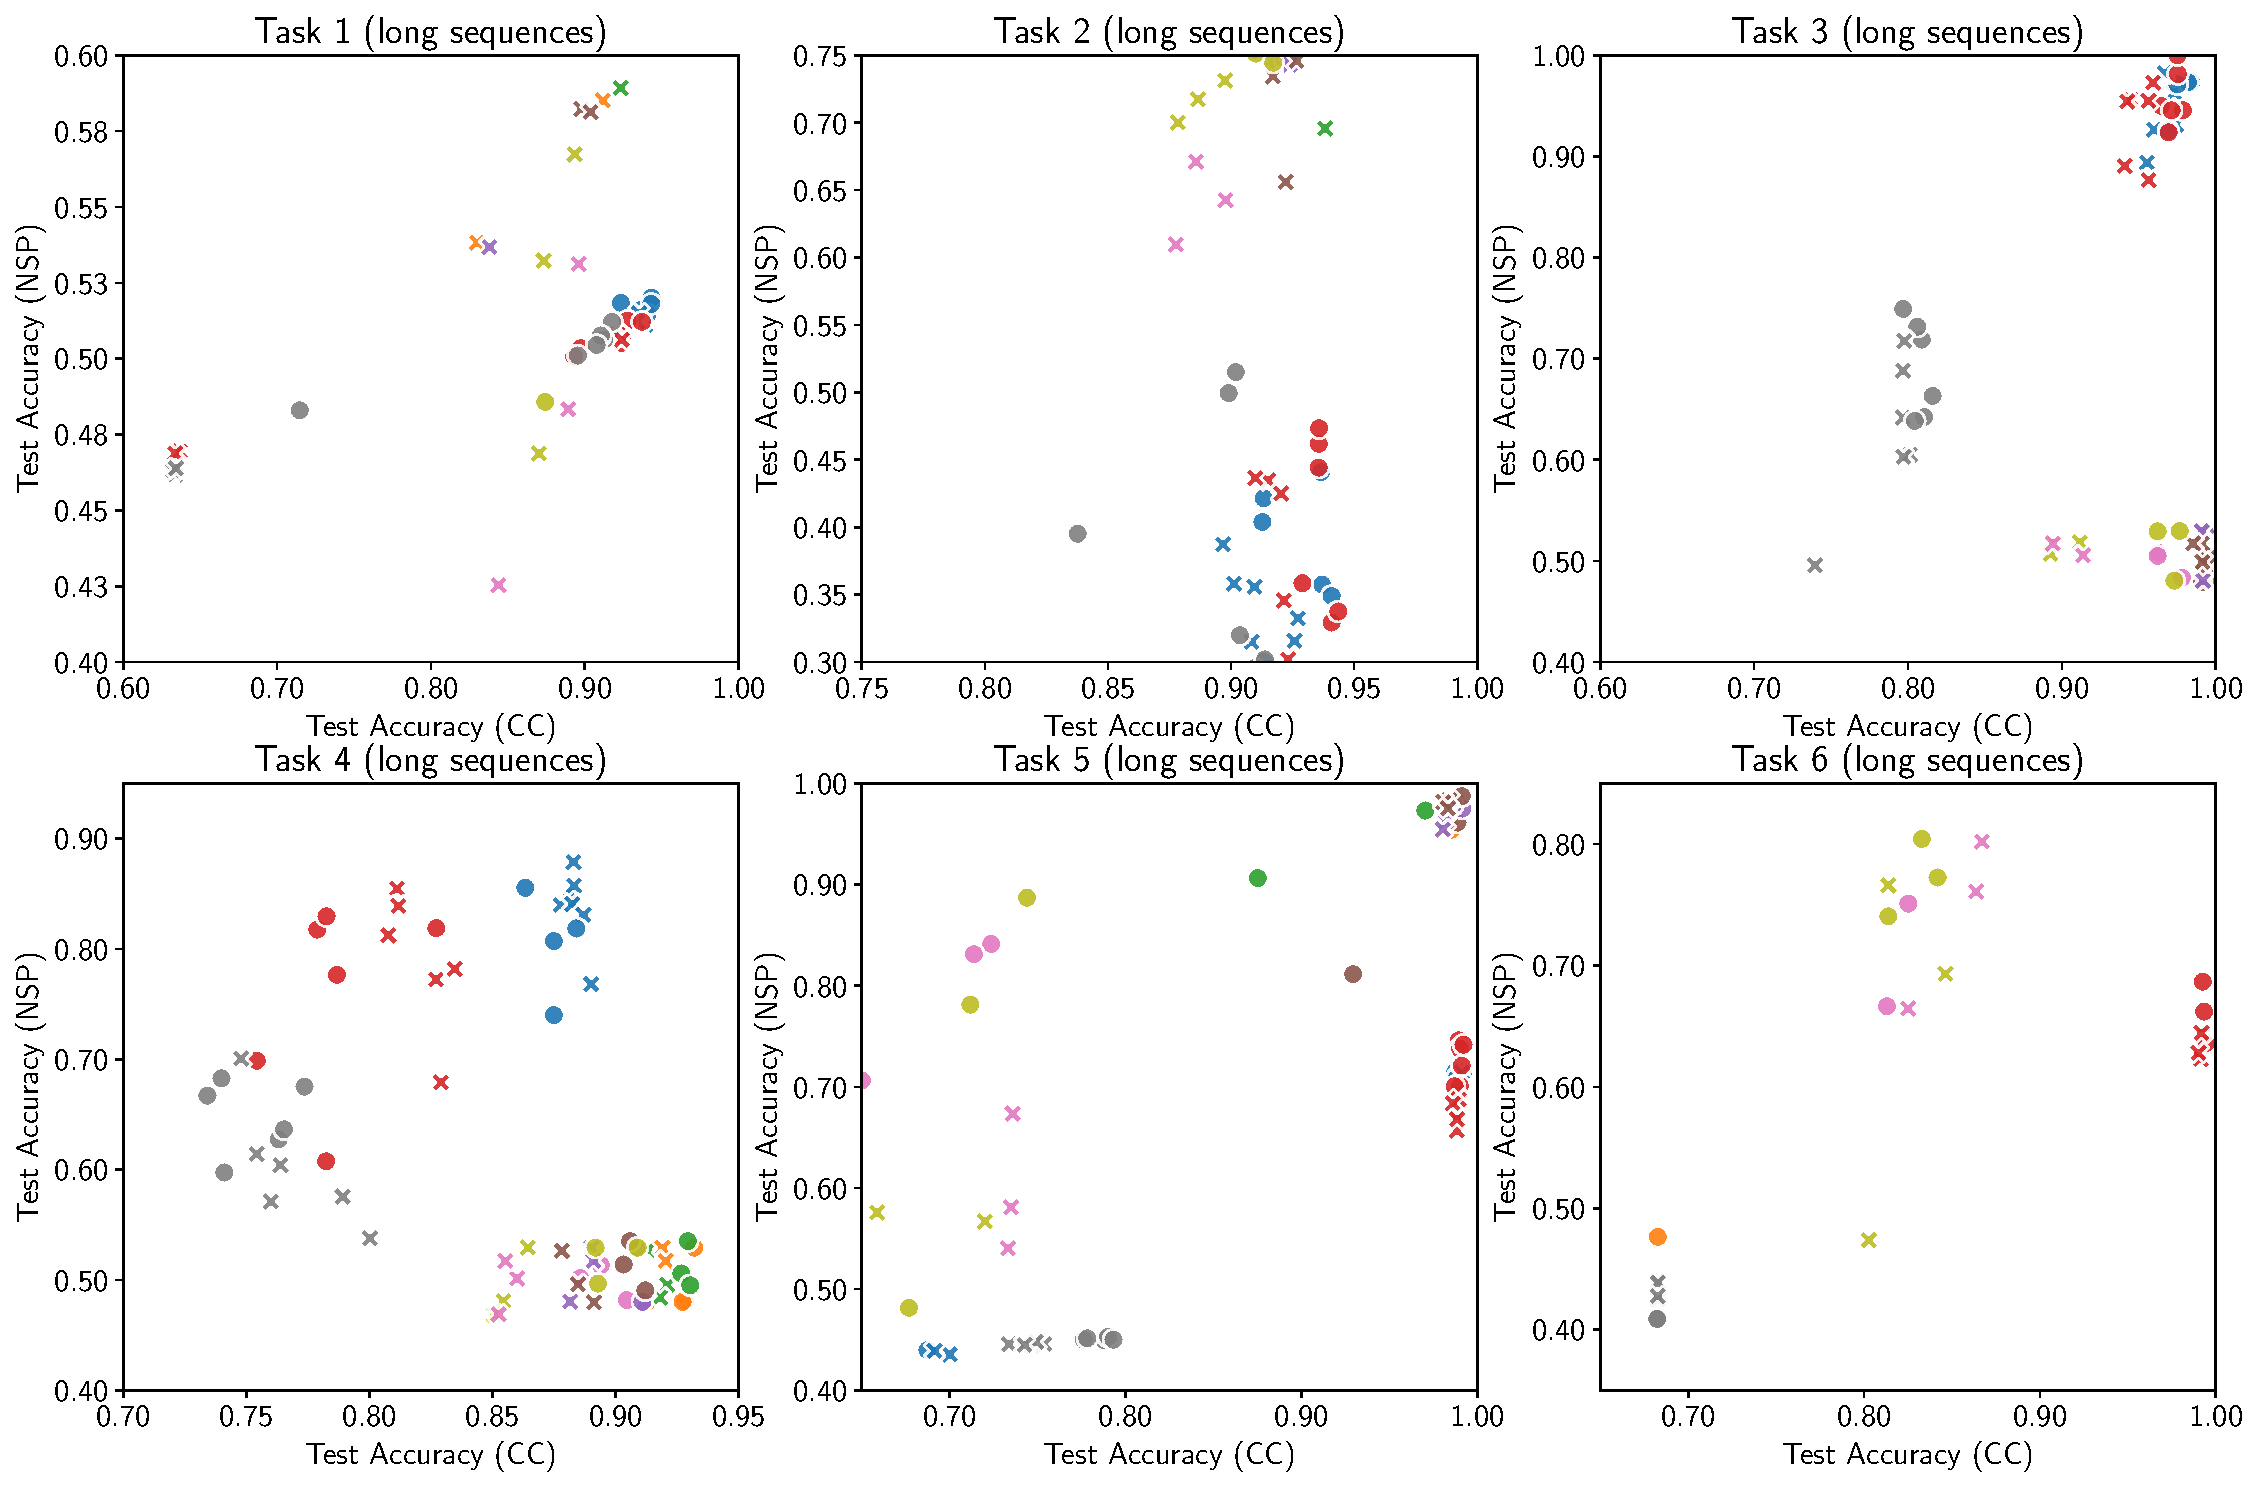
\includegraphics[width=1.0\textwidth]{imgs/ltlzinc/const-vs-succ-long.pdf}
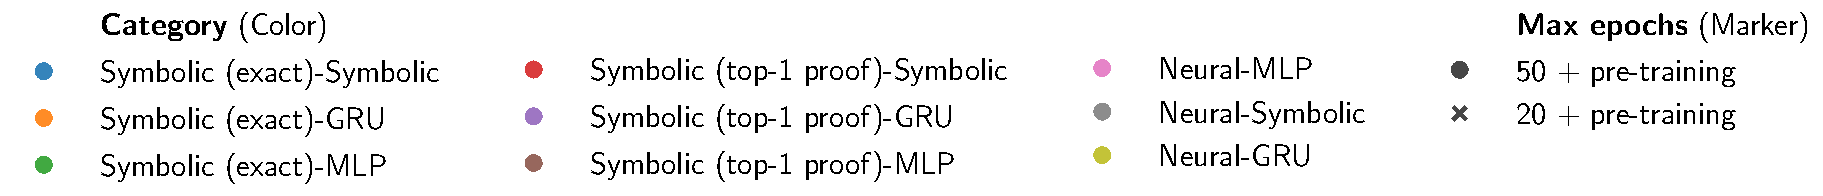
\includegraphics[width=1.0\textwidth]{imgs/ltlzinc/const-vs-succ_legend.pdf}
\caption[\textsc{cc}--\textsc{nsp} accuracy-trade-off on \textsc{LTLZinc-Sequential-Long}]{{\sc cc}-{\sc nsp} accuracy trade-off on \textsc{LTLZinc-Sequential-Long} experiments for different categories.} %Axes stretched for readability.}
\label{ltlzinc:fig:sequential-tradeoff-long}
\end{figure}



\iffalse
\section{Neuro-symbolic Experiments on \textsc{LTLZinc-Sequential-Short-Legacy}}\label{ijcai:sec:exp}
%We hereby present an experimental evaluation conducted on six LTLZinc tasks.\footnote{LTLZinc generator, our dataset, and code for full reproducibility: \url{https://github.com/continual-nesy/LTLZinc}.}
%
%Each consists in a binary classification problem on $400$ image sequences of variable length (between 10 and 20), with
%images sampled from MNIST~\cite{lecun1998mnist} and Fashion MNIST~\cite{xiao2017fmnist}.
%Tasks are annotated with relational and temporal knowledge (see Appendix~\ref{ijcai:app:tasks} for all the details).
%
\TODO{We address research questions of Section~\ref{ijcai:sec:setup} with three distinct experimental activities, aimed to study the effect of different architectures and available knowledge. Notice that our goal is not to simply find the best performing model, but to explore different scenarios and gain insights on our challenging setting.}
Appendices~\ref{ijcai:app:main}, \ref{ijcai:app:neur} and~\ref{ijcai:app:abla} report values of every hyper-parameter.
%As we are not interested in maximizing predictive performance, and to limit computational budget, we set traditional learning hyper-parameters (details in Appendices~\ref{ijcai:app:main}, \ref{ijcai:app:neur} and~\ref{ijcai:app:abla}), and study the effect of architectural differences and knowledge availability.

\paragraph{Neural-only Experiments.}
To explore neural-only methods, our modular architecture is instantiated with neural components only (i.e., the convolutional backbone (\textsc{ic}), MLP-S/L for constraint classification (\textsc{cc}), and MLP-S/L or GRU-S/L for next-state prediction (\textsc{nsp}), Fig.~\ref{ltlzinc:fig:pipeline}). Supervision is provided at every level, weighting each loss by the same positive coefficient ($\lambda_{\bullet} = 1.0$). 
%%%%
We expect the neural-only pipeline to achieve good performance in managing the \textsc{ic} stage, but also downstream performance to be negatively affected, given the limited data availability and complexity of reasoning involved.

\TODO{MERGE WITH APPENDIX AND MOVE TO RESULTS}
 \TODO{Results (detailed in Appendix~\ref{ijcai:app:neuronly}) confirmed that, despite their perceptual simplicity, no task can be effectively learned with sequence-level labels alone.} 
We experienced slow convergence and sub-optimal performance at the end of training. In fact, in spite of good overall image classification, the optimizer is often stuck in local equilibrium points, causing performance for other training objectives to plateau multiple times during training. Harder reasoning tasks exacerbate this effect. %Detailed results are reported in Appendix \ref{ijcai:app:neuronly}).

\paragraph{Neuro-symbolic Experiments.}
This second experimental batch aims to compare Neural vs. Neuro-symbolic methods, thus the effect of background knowledge over multiple reasoning steps, as well as the interaction between components.
We fix a neural perceptual backbone (\textsc{ic}), and then build four categories by combining either Neural (red, Fig.~\ref{ltlzinc:fig:pipeline}) or Symbolic (green, Fig.~\ref{ltlzinc:fig:pipeline}) modules for constraint prediction (\textsc{cc}) and temporal reasoning (\textsc{nsp}). %For brevity, we will omit the (always neural) perception module, and 
We will indicate each configuration with a shorthand notation, e.g., Symbolic-Neural means Symbolic \textsc{cc} and Neural \textsc{nsp} modules.
%
The use of the semantic loss and/or of calibration (Section~\ref{ijcai:sec:setup}), are treated as additional hyper-parameters.
Training is performed in two steps: 5 pre-training epochs for the \textsc{ic} module, and then 20 epochs of training for the entire architecture. Overall, these experiments confront 96 combinations, across 6 tasks, each seeded 3 times.
\TODO{FOR THESE EXPERIMENTS ONLY SCALLOP CC}


\paragraph{Error propagation across Symbolic Modules.}
%These experiments explicitly focus on the behavior of temporal reasoning modules, in a setting which more closely relates to traditional ``one-step'' distant supervision, to answer question Q3.
The third batch of experiments focuses on the Symbolic-Symbolic (green, Fig.~\ref{ltlzinc:fig:pipeline}) architectures only. We exploit probability calibration (Section~\ref{ijcai:sec:setup}) as the only form of learning, to minimize noise and precisely pinpoint the effect of variables such as upstream label uncertainty, and supervision ``distance'' from the reasoning component. We also consider replacing {\sc ic} and {\sc cc} modules with specific ``oracles'' returning the ground truth labels, possibly with some level of corruption. In particular, we either replace only \textsc{ic} or both \textsc{ic} and \textsc{cc}. %We will refer to the former case (an oracle for image labels followed by a Scallop program and then the temporal reasoning module under evaluation) as ``perceptual oracle'', and to the latter (an oracle for constraint labels followed by the temporal reasoning module under evaluation) as ``constraint oracle''.
%
An oracle is characterized by two hyper-parameters: how ground truth is corrupted before feeding the next module, and the amount of corruption in terms of noise probability $p$. ``Flip oracles'' return correct labels with probability $1-p$, and random labels with probability $p$, both with confidence $1.0$. ``Confidence oracles'', on the other hand, always return correct labels with random confidence between $1-p$ and $1.0$, redistributing the remaining mass to other labels.
When $p = 0.0$, both oracles yield ground truth labels with maximum confidence, referred to as ``perfect oracle''.
%We test $p \in [0.0, 0.05, 0.1, 0.2]$, for a total of 14 combinations of oracle distance, oracle nature and noise levels.
%
%
\section{Results}
\TODO{CHECK FROM HERE}

\paragraph{Neural-only Experiments.}%\label{app:neuronly}

\begin{figure*}[htb!]
	\centering
	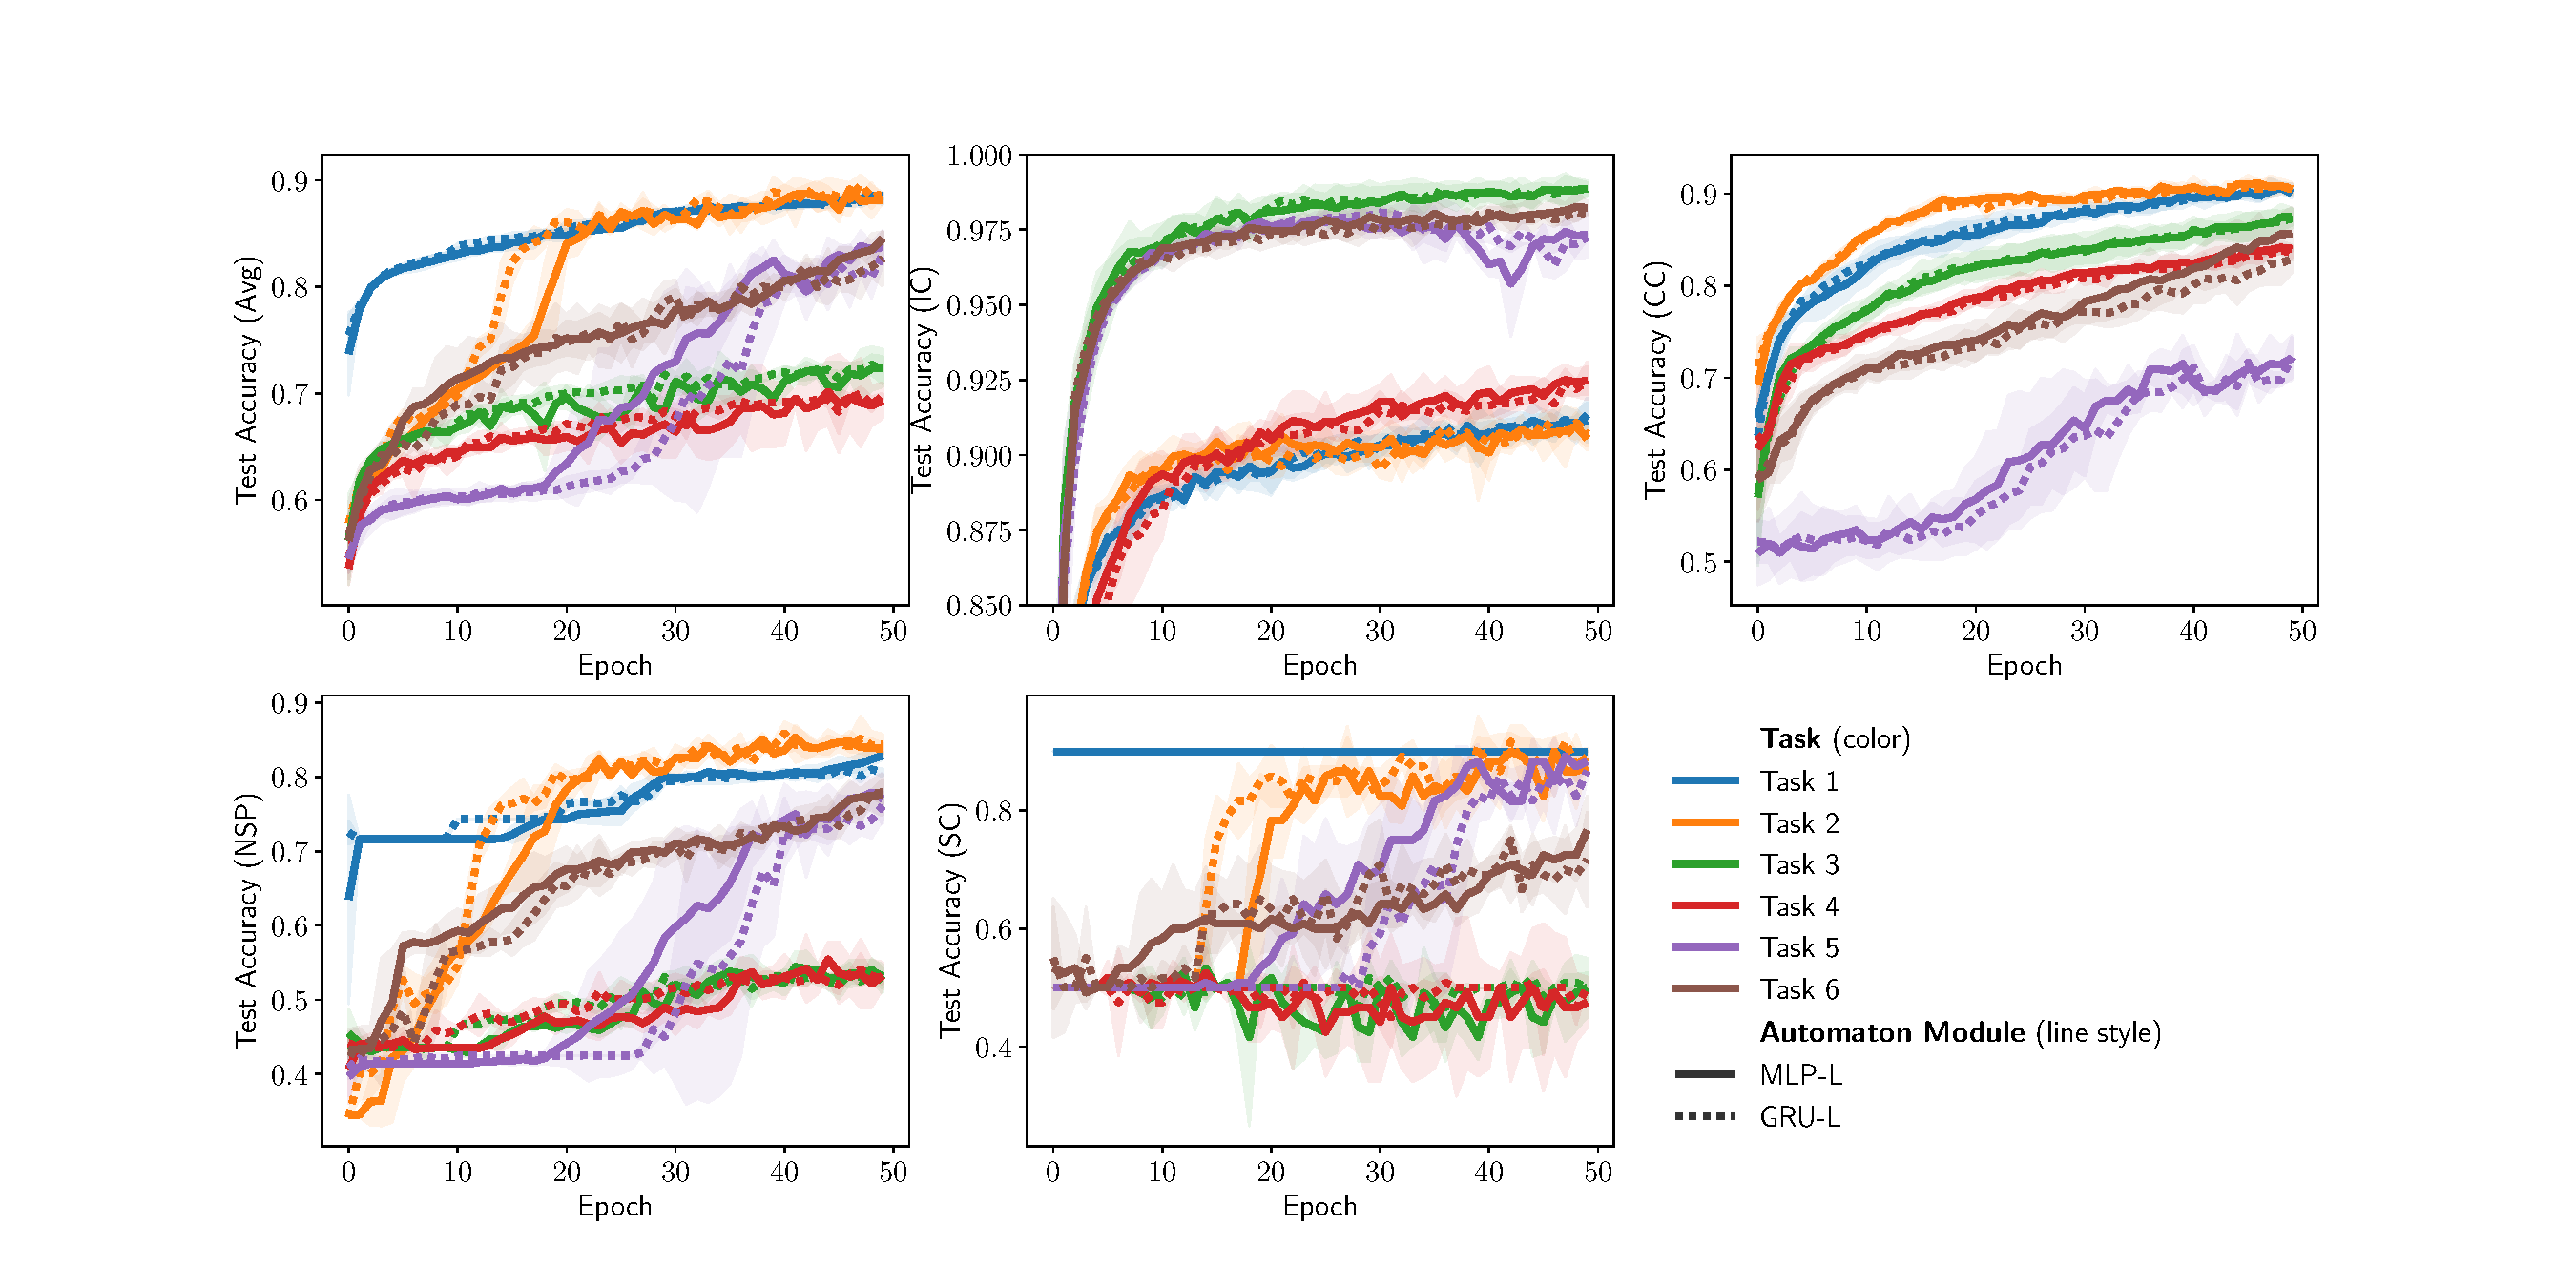
\includegraphics[width=\linewidth]{imgs/ijcai/task_validation.pdf}
	\caption{\TODO{Neural-only experiments (\textbf{Q1}).}}
	\label{fig:neural-only}
\end{figure*}

\begin{table*}[htb!]
	\centering
	\resizebox{\textwidth}{!}{
		\begin{tabular}{ccccccccc}
			\toprule
			\multirow{2}{*}{\sc Task} & \multirow{2}{*}{\shortstack[c]{\sc Automaton\\\sc Module}} & \multirow{2}{*}{\shortstack[c]{\sc Average\\\sc Accuracy}\raisebox{1ex}{\:$\uparrow$}} & \multirow{2}{*}{\shortstack[c]{\sc Label\\\sc Accuracy}\raisebox{1ex}{\:$\uparrow$}} & \multirow{2}{*}{\shortstack[c]{\sc Constraint\\\sc Accuracy}\raisebox{1ex}{\:$\uparrow$}} & \multirow{2}{*}{\shortstack[c]{\sc Successor\\\sc Accuracy}\raisebox{1ex}{\:$\uparrow$}} & \multirow{2}{*}{\shortstack[c]{\sc Sequence\\\sc Accuracy}\raisebox{1ex}{\:$\uparrow$}}
			 & \multirow{2}{*}{\shortstack[c]{\sc Most Probable\\\sc Successor Acc.}\raisebox{1ex}{\:$\uparrow$}}
			  & \multirow{2}{*}{\shortstack[c]{\sc Most Probable\\\sc Sequence Acc.}\raisebox{1ex}{\:$\uparrow$}}\\
			  & & & & & & & & \\
			\midrule
			Task 1 & MLP-L & $\textbf{0.89}$ & $0.91 $ {\tiny $\pm 0.01$} & $0.90 $ {\tiny $\pm 0.01$} & $\textbf{0.83} $ {\tiny $\pm 0.01$} & $0.90$ & $0.72$ & $0.90$\\
			Task 1 & GRU-L & $0.88$ & $0.91$ & $0.90 $ {\tiny $\pm 0.01$} & $0.81 $ {\tiny $\pm 0.01$} & $0.90$ & $0.72$ & $0.90$\\
			\midrule
			Task 2 & MLP-L & $0.88$ & $0.91$ & $0.90 $ {\tiny $\pm 0.01$} & $0.84 $ {\tiny $\pm 0.01$} & $0.88$ & $0.34$ & $0.50$\\
			Task 2 & GRU-L & $\textbf{0.89}$ & $0.91$ & $\textbf{0.91} $ {\tiny $\pm 0.01$} & $0.84 $ {\tiny $\pm 0.01$} & $\textbf{0.89} $ {\tiny $\pm 0.01$} & $0.34$ & $0.50$\\
			\midrule
			Task 3 & MLP-L & $0.72 $ {\tiny $\pm 0.02$} & $0.99$ & $\textbf{0.88} $ {\tiny $\pm 0.01$} & $0.53 $ {\tiny $\pm 0.02$} & $0.50 $ {\tiny $\pm 0.05$} & $0.45$ & $0.50$\\
			Task 3 & GRU-L & $0.72 $ {\tiny $\pm 0.01$} & $0.99$ & $0.87 $ {\tiny $\pm 0.01$} & $0.53 $ {\tiny $\pm 0.02$} & $0.50 $ {\tiny $\pm 0.02$} & $0.45$ & $0.50$\\
			\midrule
			Task 4 & MLP-L & $0.69 $ {\tiny $\pm 0.02$} & $0.92$ & $0.84$ & $0.53 $ {\tiny $\pm 0.02$} & $0.47 $ {\tiny $\pm 0.04$} & $0.45$ & $0.50$\\
			Task 4 & GRU-L & $\textbf{0.70}$ & $0.92 $ {\tiny $\pm 0.01$} & $0.84 $ {\tiny $\pm 0.01$} & $0.53 $ {\tiny $\pm 0.01$} & $\textbf{0.50}$ & $0.45$ & $0.50$\\
			\midrule
			Task 5 & MLP-L & $\textbf{0.84} $ {\tiny $\pm 0.02$} & $0.97 $ {\tiny $\pm 0.01$} & $0.72 $ {\tiny $\pm 0.02$} & $\textbf{0.77} $ {\tiny $\pm 0.03$} & $\textbf{0.88} $ {\tiny $\pm 0.01$} & $0.41$ & $0.50$\\
			Task 5 & GRU-L & $0.83 $ {\tiny $\pm 0.01$} & $0.97$ & $0.72 $ {\tiny $\pm 0.02$} & $0.76 $ {\tiny $\pm 0.02$} & $0.87 $ {\tiny $\pm 0.01$} & $0.41$ & $0.50$\\
			\midrule
			Task 6 & MLP-L & $\textbf{0.85} $ {\tiny $\pm 0.01$} & $0.98$ & $\textbf{0.86} $ {\tiny $\pm 0.03$} & $0.78 $ {\tiny $\pm 0.03$} & $\textbf{0.77} $ {\tiny $\pm 0.06$} & $0.45$ & $0.50$\\
			Task 6 & GRU-L & $0.83 $ {\tiny $\pm 0.03$} & $0.98$ & $0.83 $ {\tiny $\pm 0.02$} & $0.78 $ {\tiny $\pm 0.02$} & $0.72 $ {\tiny $\pm 0.08$} & $0.45$ & $0.50$\\
			
			\bottomrule
		\end{tabular}
	}
	\caption{\TODO{Aggregated test accuracies for each task (purely neural experiments, \textbf{Q1}). Values are reported as $mean \pm st. dev$, aggregated over 3 random seeds. Standard deviations are omitted if smaller than $10^{-2}$. MP: Most probable predictor.}}
	\label{tab:neural-only}
\end{table*}

Figure \ref{fig:neural-only} and Table \ref{tab:neural-only} highlight the results of neural-only experiments.
In spite of the large training capacity, neural-only methods are characterized by slow convergence. In terms of average performance, only the simplest tasks (task 1, blue lines, and task 2, orange lines) achieve relatively high values by the end of training, with other tasks either plateauing at values close to random performance (tasks 3 and 4, green and red lines, respectively), or still far from convergence at the end of training (tasks 5 and 6, purple and brown). Some steep boosts in performance during training (e.g., tasks 2, between epochs 10-20, and 5, between epochs 20-40) might hint at optimization challenges.
%
\textsc{IC} performance is good for every task and it does not appear to be a bottleneck for performance. Tasks 3, 5 and 6 achieve near perfect classification accuracy, as they are characterized by values sampled from the MNIST digits domain, while the perceptually harder tasks 1, 2 and 4 are sampled from Fashion-MNIST, and still achieve $>0.9$ accuracy by the end of training.
%
In general there seem to be no difference between an \textsc{NSP} module implemented as multi-layer perceptron (MLP, solid lines) and one implemented with gated recurrent units (GRU, dotted lines). However, the harder-to-optimize tasks 2 and 5 present distinct training dynamics, with GRU converging in fewer epochs for task 2, while being slower for task 5. Task 2 is characterized by the necessity of ``keeping in memory'' a large temporal horizon (4 time steps, thus being easier for a recurrent architecture), albeit on perceptually simple constraints, while task 5 is a simple alternation of a complex (arithmetic) constraint being satisfied and then violated cyclically (thus architectural choice becomes irrelevant and feed-forward approaches, characterized by fewer learnable parameters, converge faster). There seem to be no backward interference of temporal modules on constraint and label accuracy, which are completely unaffected.
%
\textsc{CC} accuracy is generally good, with the exception of task 5, which cannot achieve satisfiable performance by the end of training. This task is characterized by a single arithmetic constraint in the form $A + B = C + D$, for which neural networks struggle. The initial random guessing phase corresponds to the first plateau in overall performance (epochs 0-20), as downstream objectives are conditioned on constraint prediction. Afterwards, in spite of low predictive performance at the \textsc{CC} level, the simple temporal behavior allows to achieve good \textsc{NSP} (and therefore average as well) accuracy in spite of an high rate of mispredicted constraints.
%
\textsc{NSP} is challenging for tasks 3 and 4, which do not improve over random guessing. Task 1 plateaus almost immediately, while tasks 2 and 5 are characterized by a slow start. Poor upstream predictive performance negatively affects task 5 at the beginning, while task 2 is subject to harder to optimize long-range temporal behavior.

\subsection{The Impact of Neuro-Symbolic Approaches}
\begin{figure*}
\centering
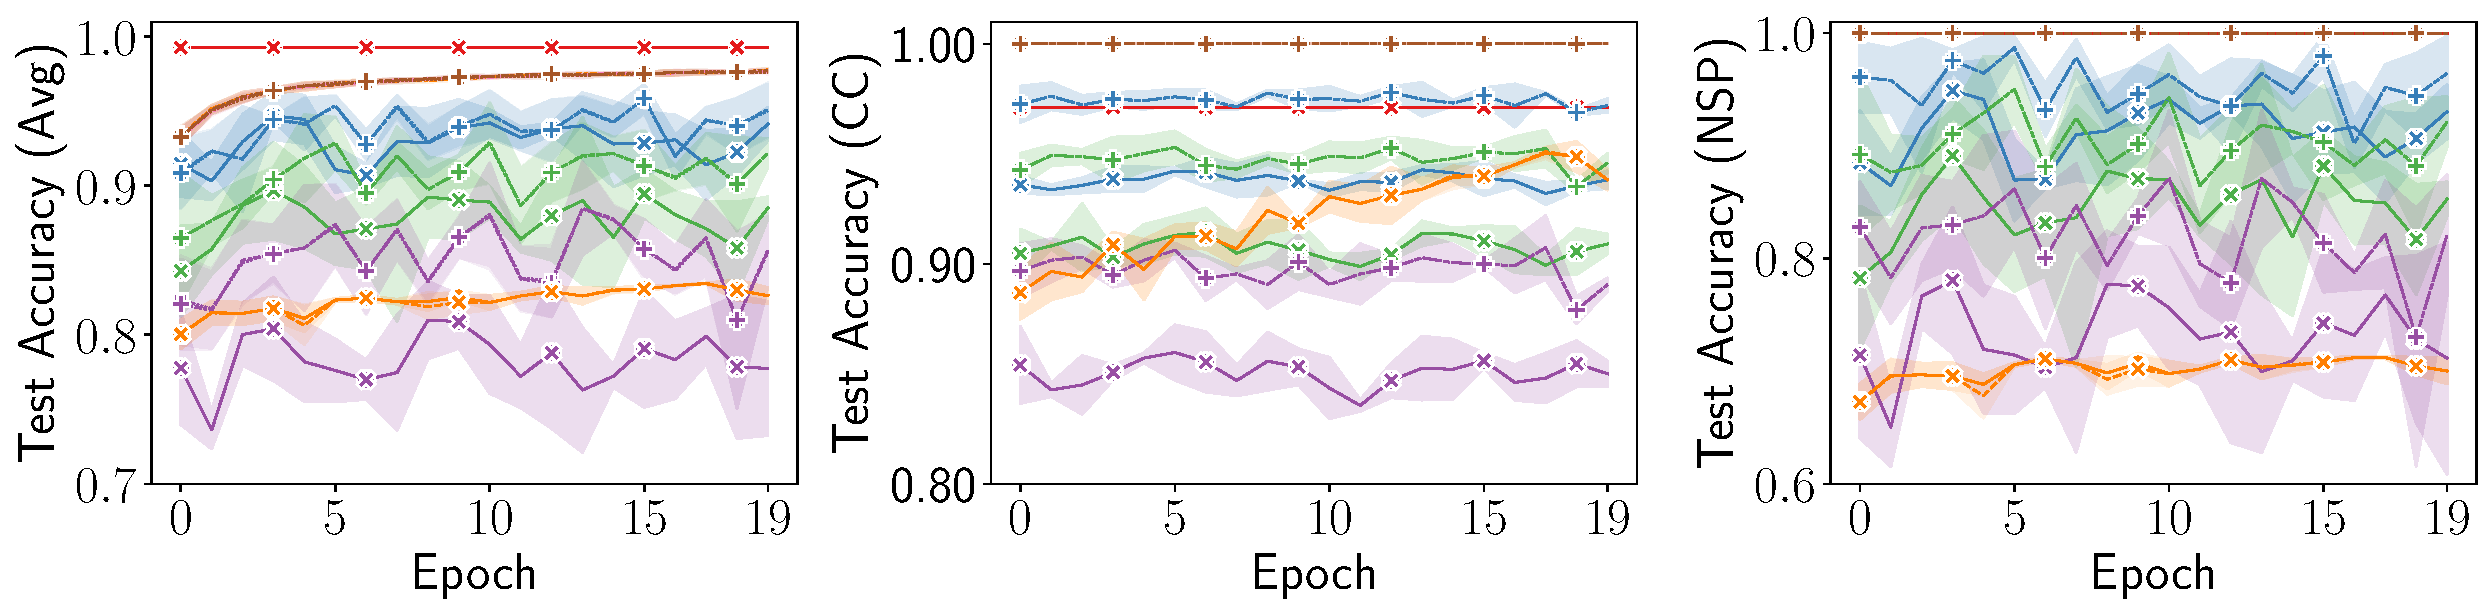
\includegraphics[width=\linewidth]{imgs/ijcai/ablation_task4.pdf}\\
{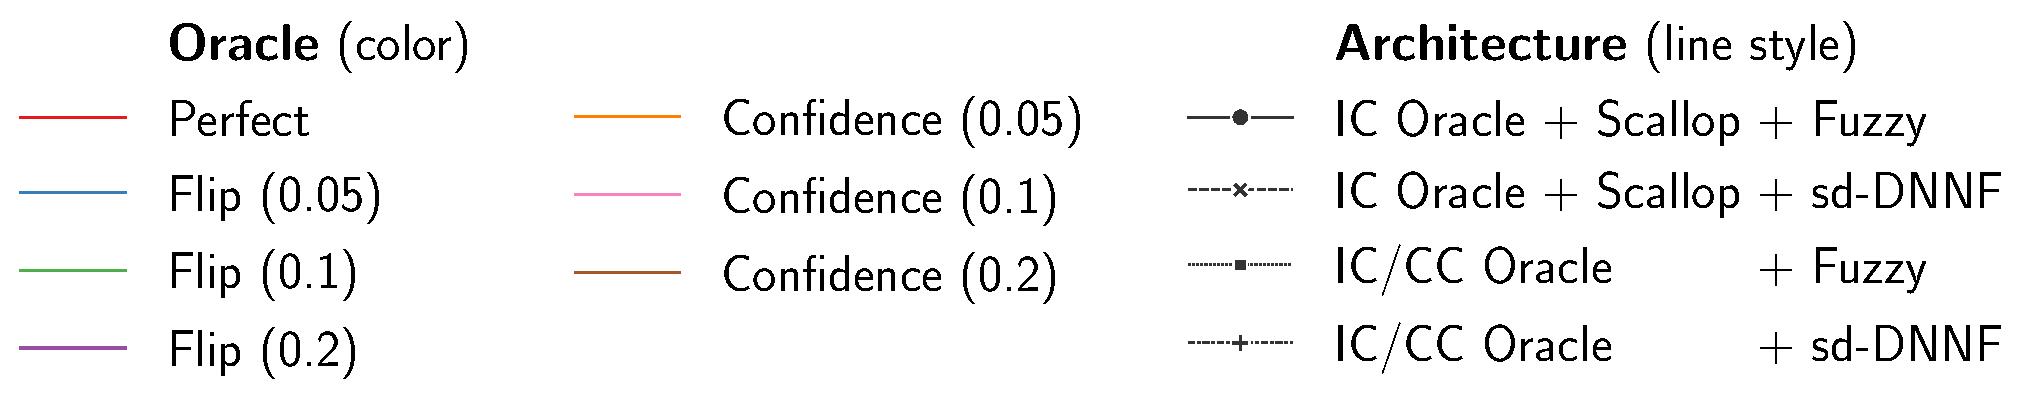
\includegraphics[width=\linewidth]{imgs/ijcai/ablation_task4_legend.pdf}}
\caption[Oracle experiments on LTLZinc-Short (rejection sampling) Task 4]{\textbf{Q3}. Accuracies for \textit{Task 4} with oracular predictors. Oracle types (perfect, flip, confidence) are described in Section~\ref{ijcai:sec:exp}.}
\label{ijcai:fig:abl-task4}
\end{figure*}
%
Fig.~\ref{ijcai:fig:main} highlights the trade-offs between \textsc{cc} and \textsc{nsp}, as a function of the different Neural/Symbolic implementations.
%
Exploiting a symbolic component both for \textsc{cc} and \textsc{nsp} (Symbolic-Symbolic, brown points) allows to achieve the best trade-off for every task considered. Unlike other combinations, these approaches consistently outperform naive baselines which always return the most probable class observed in the training set, both for \textsc{nsp} (dashed horizontal line), and \textsc{cc} (not shown, outside the left boundary of plots).
%
The additional learning capacity provided by temperature calibration (dots vs. crosses) has an overall limited effect.
%
With the exception of tasks 1, 2 and 4, neural modules for \textsc{nsp} (clusters Symbolic-MLP/GRU and Neural-MLP/GRU, blue, orange, red and purple) achieve unsatisfactory performance, even when fed from highly-accurate symbolic \textsc{cc} predictions. These architectures, at times, perform on par with the most probable guessing baseline, and often below it.
%
Symbolic modules for \textsc{nsp} are characterized by a large dispersion, due to optimization challenges: this is especially true when exploiting neural \textsc{cc} modules (Neural-Symbolic, green), but it can also be observed in combination with symbolic \textsc{cc} modules (Symbolic-Symbolic, brown). Conversely, neural \textsc{nsp}, even though often showing unsatisfactory performance, is characterized by a much smaller inter-experiment variance.
%
%Comparing different tasks, it can be observed that tasks 1 and 2 can be solved by most combinations of modules (with fully neural approaches, blue and orange points, struggling the most), while both relational and temporal knowledge are crucial for every other task.
%
%
Table~\ref{ijcai:tab:main} summarizes performance for each task. %Experiments are replicated three times, to evaluate variance caused by different initialization.
%
Overall, the Symbolic-Symbolic category dominates over other groups, with the exception of task 5, where it performs slightly worse than the Symbolic-Neural family. When observing constraint accuracy alone, a downstream Symbolic \textsc{nsp} module often negatively affects performance, with task 4 presenting the highest delta between Symbolic-Symbolic and Symbolic-Neural.
Conversely, when focusing on next state prediction, an upstream Symbolic \textsc{cc} module is beneficial to a downstream Symbolic temporal reasoning module, however this clear-cut performance improvement is flipped when the \textsc{nsp} module is Neural. This behavior hints at complex interactions between \textsc{cc} and \textsc{nsp} modules, where architectural choices bi-directionally affect both components.
%
%No clear trend in the effect of other hyper-parameters can be identified. 
Other hyper-parameters have negligible effect. 
Early stopping is almost always triggered near the end of training, hinting at a possibly incomplete convergence. Temperature calibration is often selected, but performance improvements are minor (cfr. with Fig. \ref{ijcai:fig:main}), and the semantic loss proposed by~\cite{umili2023grounding} is not significantly different than traditional binary cross-entropy in our setting.
%
Variances across three runs for each set of hyper-parameters are low. Comparing this observation to Fig.~\ref{ijcai:fig:main} (which, instead, highlights hyper-parameter-based variance), it can be observed that convergence in multi-stage neuro-symbolic sequence classification is heavily dependent on architectural choices, but relatively unaffected by parameter initialization.
%
Task 3 is an exception and it presents a failure case of the Symbolic-Symbolic family, due to training instability. When able to converge, however, it is the only approach capable of improving over random guessing for sequence classification for this task (we reported this sample result surrounding the model name with brackets).


\subsection{The Impact of Oracular Predictors}
Fig.~\ref{ijcai:fig:abl-task4} shows the effect on an exemplar task (Task 4) of oracular predictors on symbolic temporal reasoning modules.
Figures \ref{ijcai:fig:abl-avg}, \ref{ijcai:fig:abl-const} and \ref{ijcai:fig:abl-succ}, in the supplementary materials, show the same plots for every task.
%
In general, the trainable temperature parameters are quickly optimized, with curves following a mostly horizontal trend. However, flip oracles (blue, green and purple lines) are characterized both by larger variance and inter-epoch oscillations, compared to confidence oracles (orange, pink and brown), which present a remarkably stable behavior. This effect is present in every task, regardless of reasoning difficulty.
%
Noise injection, however, affects the two oracles differently: performance for flip oracles degrades linearly when increasing noise, while confidence oracles are characterized by non-linear behavior. Small amounts of noise do not affect confidence oracles appreciably, while larger amounts tend to harm performance more than the flip oracle. This effect is more evident for harder reasoning tasks: for instance, in task 4, a noise of $p = 0.1$ is enough to cause random guessing performance (Fig. \ref{ijcai:fig:abl-task4-nolimits} in the Appendix).
%
\iffalse
The effect of different automata encodings on \textsc{IC} oracles is virtually non-existent (overlapped dot and cross markers), while \textsc{IC/CC} oracles are relatively more robust to noise when the \textsc{nsp} module employs sd-DNNF (dot-dash lines), compared to a fuzzy (dotted) encoding. This behavior may be a result of the symbolic \textsc{cc} module filtering-out noise in \textsc{IC} oracles, bypassed in constraint-level oracles.
\fi
With oracles, the effect of different automata encodings is virtually non-existent (fuzzy and sd-DNNF markers overlap almost everywhere). 
%
\textsc{IC} oracles are consistently more affected by noise, compared to \textsc{IC/CC} ones. This behavior seems counterintuitive, as the Scallop module performs near-exact inference; however, it is in line with the hypothesis of uncertainty accumulation over multiple steps of reasoning.
%
When focusing on constraint performance (Fig.~\ref{ijcai:fig:abl-const} in the supplementary materials), flip oracles tend to have stable performance, while confidence oracles can exploit temperature parameters to achieve a small learning capacity (slight upward trend across epochs).
In general, flip oracles are more robust to noise, with confidence oracles achieving unsatisfactory performance (outside plot boundaries, see Fig. \ref{ijcai:fig:abl-task4-nolimits} in the Appendix) for harder tasks or higher ($p > 0.05$) degrees of uncertainty.
This behavior clashes with the desirable property of predictive confidence correlating with uncertainty, which is one of the advantages of neuro-symbolic AI, compared to (uncalibrated) neural networks. Flip oracles achieving better performance than confidence oracles, for similar levels of noise, hint at the fact that an overconfidently-wrong classifier can be more successful than a reluctantly-correct one, in temporal reasoning settings.
%
%Regarding performance on successor prediction (Fig. \ref{ijcai:fig:abl-succ}), the choice of automaton encoding does not play any role (solid and dotted, dashed and dot-dashed lines overlap each other for almost every data point), hinting at the fact that performance degradation due to upstream predictive noise is not affected by the presence of neutral and disjoint sum problems, however, as noted previously, a probabilistic semantics (sd-DNNF encoding) can be beneficial on upstream constraint prediction performance, possibly due to more stable gradients computed during backpropagation.
%
%The small positive slope identified in constraint prediction for confidence oracles does not propagate to next state prediction, where both flip and confidence oracles present an horizontal trend. At the same time, however, confidence oracles are characterized by a smoother training progression and lower inter-experiment variance, as it was the case for constraint prediction.
\fi
\iffalse
\section{Conclusions}
We extended knowledge-driven sequence classification to a relational setting, introducing a novel benchmarking framework and baselines for neural-only and multi-stage neuro-symbolic methods in a knowledge-driven, and long-temporal-horizon regime.
%
Experiments outline a challenging setting, where neural networks struggle to generalize and state-of-the-art neuro-symbolic methods fall short when stacked: temporal reasoners extended to a relational domain can fail even with full background knowledge available, and general-purpose first-order reasoners suffer from training instabilities in recurrent settings.
%
We argue that the proposed benchmarking framework can benefit the neuro-symbolic and temporal reasoning communities, further pushing research boundaries towards more expressive frameworks, tighter neuro-symbolic integration, and more robust time-driven approaches.
\fi